\newtcolorbox{perfbox}[2][]{enhanced,
    boxrule=0.5pt,
    colframe=black,
    colback=white,
    sharp corners,
    fonttitle=\bfseries,
    attach boxed title to top left={xshift=2mm,yshift*=-\tcboxedtitleheight/2},
    boxed title style={
        size=small,
        colframe=black,
        colback=black,
        sharp corners,
        boxrule=0.5pt
    },
    title=#2,#1
}

\chapter{Evaluation}\label{chapter:evaluation}

In the previous chapters, some variate generators included in common frameworks were briefly presented, as well as the underlying 
algorithms used to sampled the Zipfian distribution. To make a fair comparison, it's necessary to evaluate the accuracy of the distributions generated, 
as well as the performance of the algorithms used to generate them. Additionally, simplicity of the methods will be considered. 

\begin{itemize}
    \item \textbf{Accuracy}: The statistical properties of the generated distributions will be compared to the expected values given by the theoretical Zipfian distribution
    \item \textbf{Performance}: The time taken to generate the distributions will be measured and compared using standard profilling tools as well as custom-written benchmarks
\end{itemize}

The variate generators considered for this approach are exactly those presented in the previous chapters: \ac{YCSB}, \ac{FIO}, Sysbench and OLTP-Bench (which will be aliased by Rejection-Inversion - Java), along with
implementations of the algorithms discussed in \ref{chapter:approach}: Rejection and Condensed Table Lookup. Rejection-Inversion wasn't separately implemented since Sysbench already does it.

\section{Experimental Setup}

This section describes the hardware and software environment used to conduct the experiments. All experiments described in this chapter were conducted on a machine with the specifications detailed in table \ref{tab:computer-specs}.
The software environment used is detailed in table \ref{tab:software-environment}.
Since the samplers were implemented in different languages, it's also necessary to detail the versions of the interpreters used to run them (see \ref{tab:interpreter-versions}).

\begin{table}[t]
    \centering
    \begin{tabularx}{\linewidth}{>{\raggedright\arraybackslash}X >{\raggedright\arraybackslash}X >{\raggedright\arraybackslash}X >{\raggedright\arraybackslash}X >{\raggedright\arraybackslash}X}
        \hline
        \textbf{CPU Model} & \textbf{Clockspeed} & \textbf{Number of Cores} & \textbf{Memory Capacity} & \textbf{Memory Speed} \\
        \hline
        AMD Ryzen 7 5850U & 3.6 GHz & 8 & 16 GB & 3200 MHz \\
        \hline
    \end{tabularx}
    \caption{Computer Specifications}\label{tab:computer-specs}
\end{table}

\begin{table}[t]
    \centering
    \begin{tabularx}{\linewidth}{X X X X}
        \hline
        \textbf{Operating System} & \textbf{Kernel Version} & \textbf{Relevant Tools} \\
        \hline
        Debian GNU/Linux 12 & 6.1.0-amd64 & perf\cite{PerfLinuxProfilinga}, JMH \cite{AvoidingBenchmarkingPitfalls}, Google Benchmark \cite{GoogleBenchmarkMicrobenchmark}\\ 
    \end{tabularx}
    \caption{Software Specification}\label{tab:software-environment}
\end{table}


\begin{table}[ht!]
    \centering
    \begin{tabularx}{\linewidth}{>{\raggedright\arraybackslash}X >{\raggedright\arraybackslash}X >{\raggedright\arraybackslash}X}
        \hline
        \textbf{Language/Version} & \textbf{Compiler} &\textbf{Benchmark/Sampler} \\
        \hline
        C++20 & gcc 12.2.0 & Own implementation\\
        \hline
        Java 17 & OpenJDK 17.0.8 & YCSB \\
        \hline
        C (GNU17) & gcc 12.2.0 & Sysbench, FIO \\
        \hline
        Rust & 1.58.0 & None \\
    \end{tabularx}
    \caption{Interpreter Versions}\label{tab:interpreter-versions}
\end{table}

\section{Methodology}
Evaluations were conducted both for accuracy and performance. 
\paragraph{Accuracy} To measure accuracy 2 quantifiable criteria will be used
to offer well-rounded view of the quality of the generated distributions - the \textbf{Kolmogorov-Smirnov test} and the \textbf{Total Variation Distance} as explained
previously in \ref{chapter:background}. All of these are well explored in the literature \cite{clausetPowerlawDistributionsEmpirical2009,leydoldErrorDetectionNonUniforma,dengRobustnessNonuniformRandom1992,monahanAccuracyRandomNumber1985}. 

Besides these numerical quantities, a qualitative approach will be also taken to ensure the measures can be well interpreted. To this end, two visual techniques will also be
used: a \textbf{log-scaled graph} (see \ref{fig:loglog_zipf}) and a \textbf{frequency ratio analysis}. These help identify systematic deviations as well as deviations correlated 
with the rank of the indexes. Table \ref{tab:criteria} gives an overview of the criteria used for the evaluation and how each simulation was run.

\begin{table}[h]
    \centering
    \begin{tabular}{|l|l|l|l|}
        \hline
        \textbf{Criteria} & \textbf{Support Size} & \textbf{Skew} & \textbf{Number of Samples} \\
        \hline
        Log-scaled graph & $10^6$ & 0.8 & $10^9$ \\
        \hline
        Frequency Ratio Analysis & $10^6$ & 0.8 & $10^9$ \\
        \hline
        Kolmogorov-Smirnov Test & $10^8$ & 0.8 & $10^4$ to $10^9$ \\
        \hline
        Total Variation Distance & $10^8$ & 0.8 & $10^4$ to $10^9$ \\
        \hline
    \end{tabular}
    \caption{Simulation specification for each accuracy criteria}\label{tab:criteria}
\end{table}


\paragraph{Performance} The main measure of interest is \textit{throughput} - the amount of variates generated in a time interval (e.g. $10M/ms$). Since benchmarking in modern systems is a rife with
pitfalls \cite{AvoidingBenchmarkingPitfalls,beyerBenchmarkingResourceMeasurement2015}, some precautions should be taken before running the code. More details follow in the coming sections.

\section{Evaluating accuracy}
To first identify which distributions are very wrong, a simple visual inspection is done of the graphs in Figure \ref{fig:pmf-graphs}.  The only distributions which visibly deviate from the expected curve are the FIO and the Condensed Table Lookup. These will be investigated later on. 

\begin{figure}[H]
    % First row
    \centering
    \begin{subfigure}{0.46\textwidth}
        \centering
        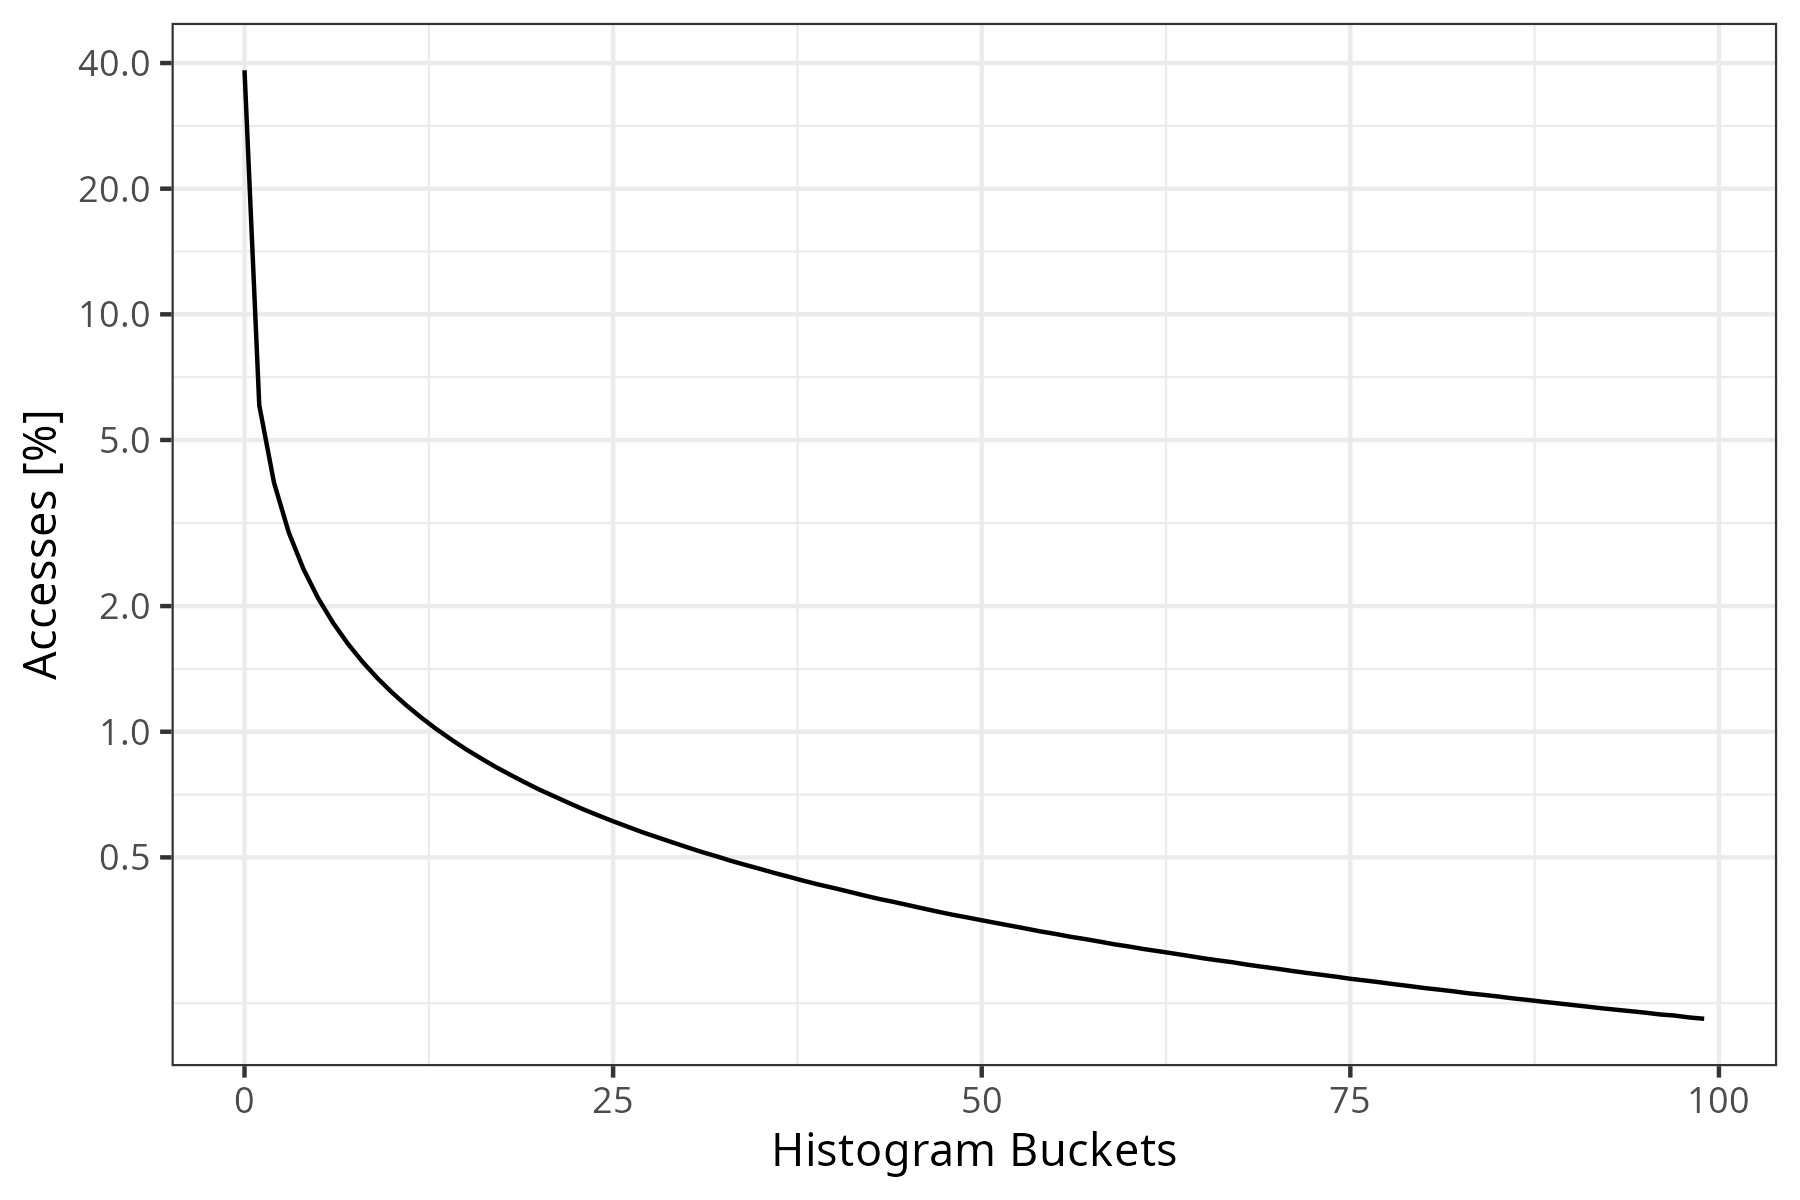
\includegraphics[width=\textwidth]{figures/pmf/apache.png}
        \caption{Rejection inversion}
    \end{subfigure}
    \hfill
    \begin{subfigure}{0.46\textwidth}
        \centering
        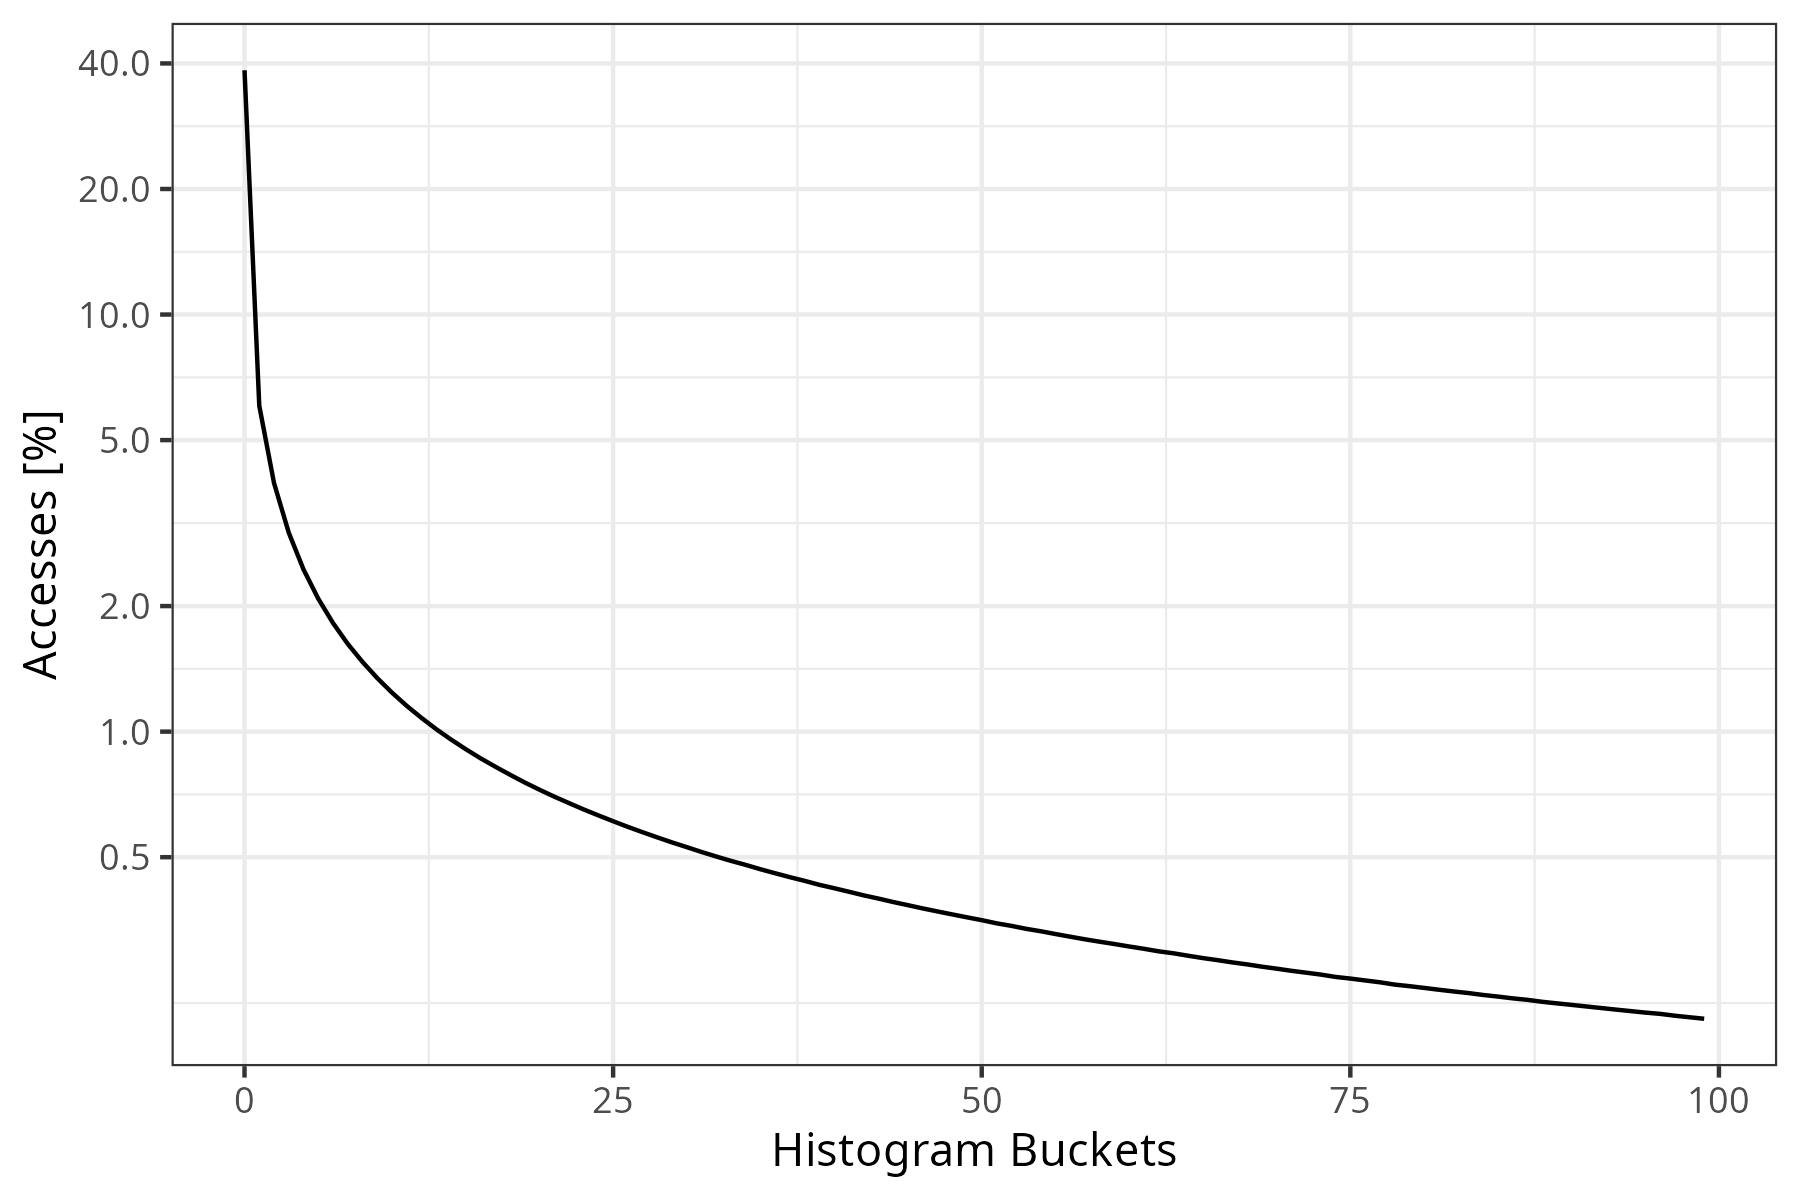
\includegraphics[width=\textwidth]{figures/pmf/ycsb.png}
        \caption{YCSB}
    \end{subfigure}
    \\ 
    % Second row
    \begin{subfigure}{0.46\textwidth}
        \centering
        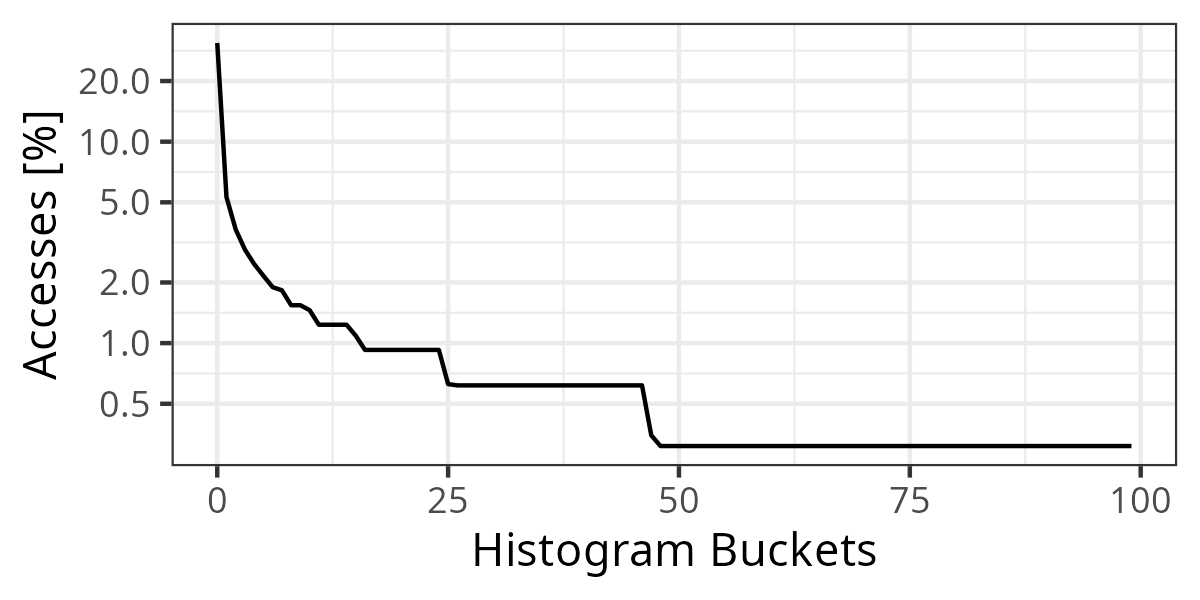
\includegraphics[width=\textwidth]{figures/pmf/fio.png}
        \caption{FIO}
    \end{subfigure}
    \hfill
    \begin{subfigure}{0.46\textwidth}
        \centering
        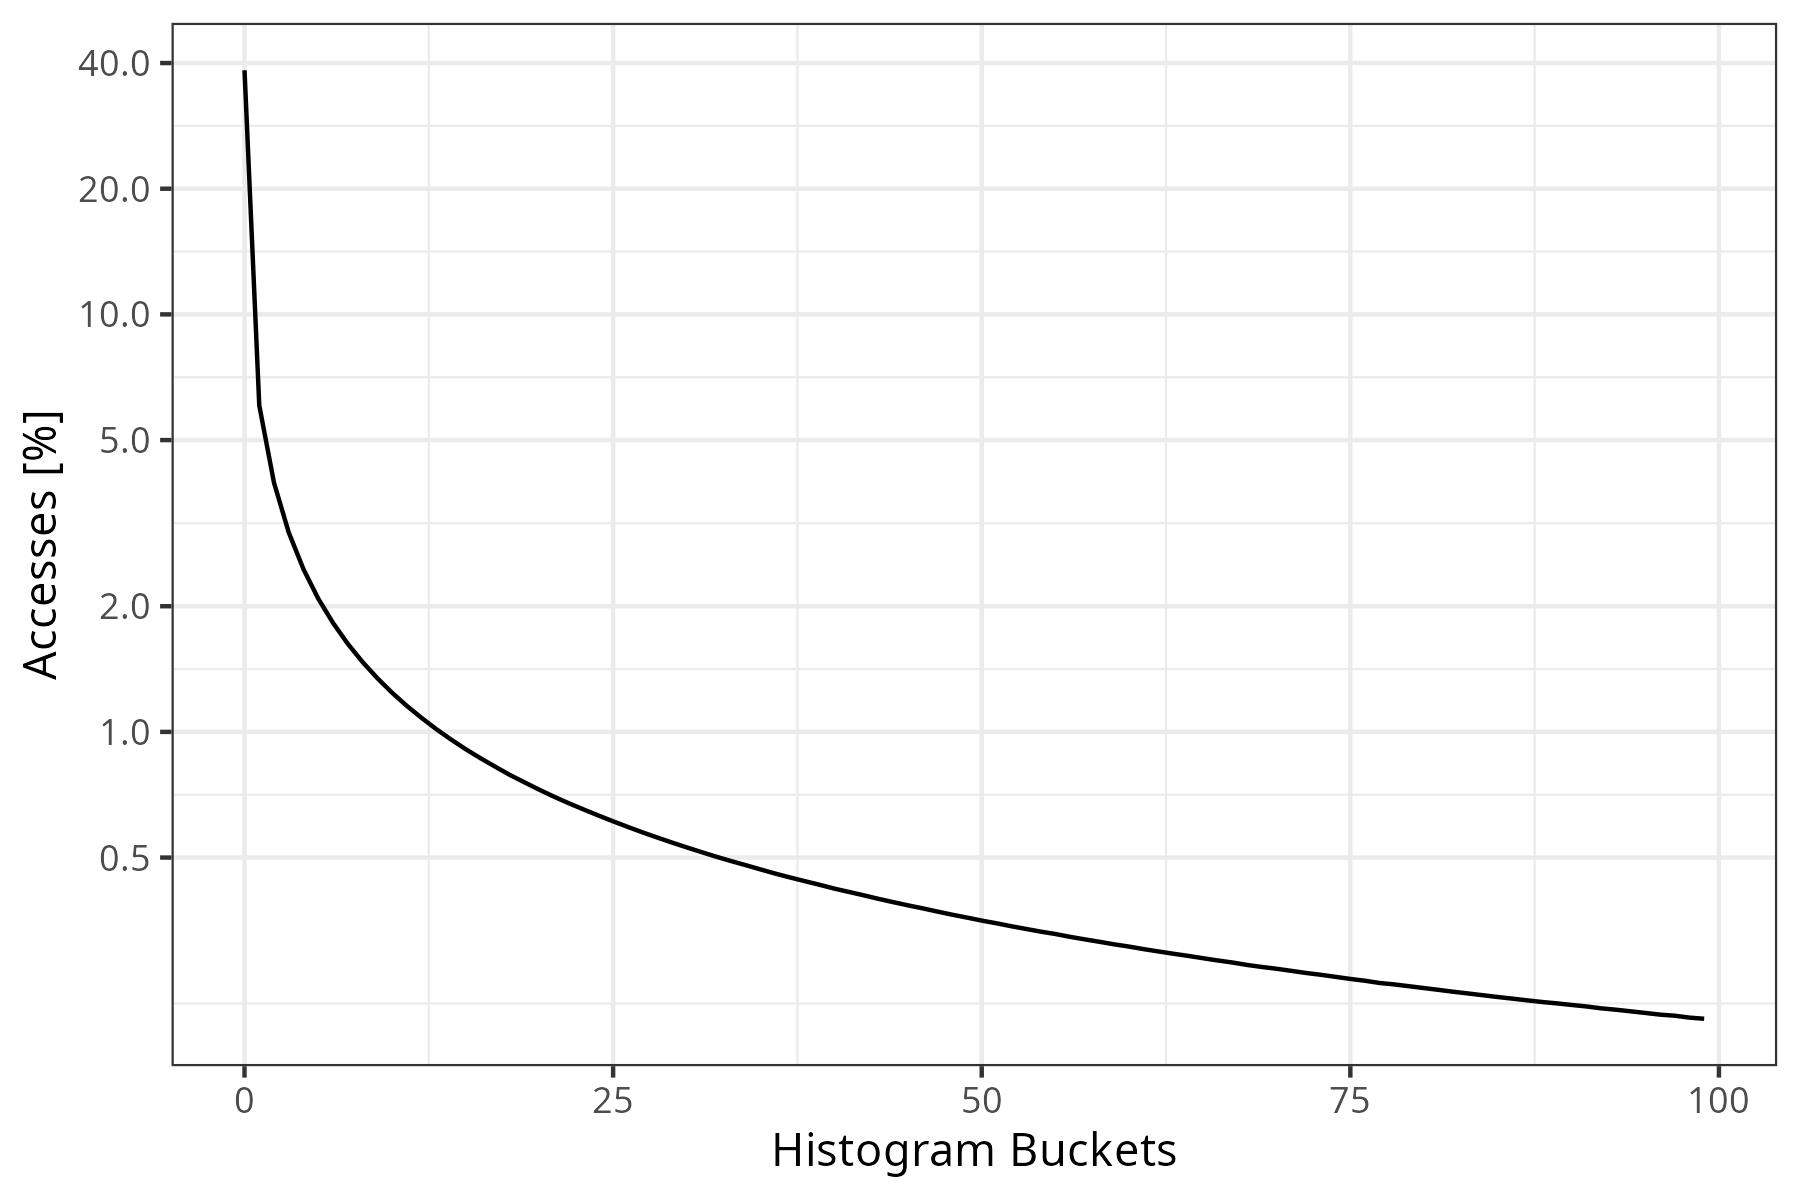
\includegraphics[width=\textwidth]{figures/pmf/sysbench.png}
        \caption{Sysbench}
    \end{subfigure}
    \\    
    % Third row
    \begin{subfigure}{0.46\textwidth}
        \centering
        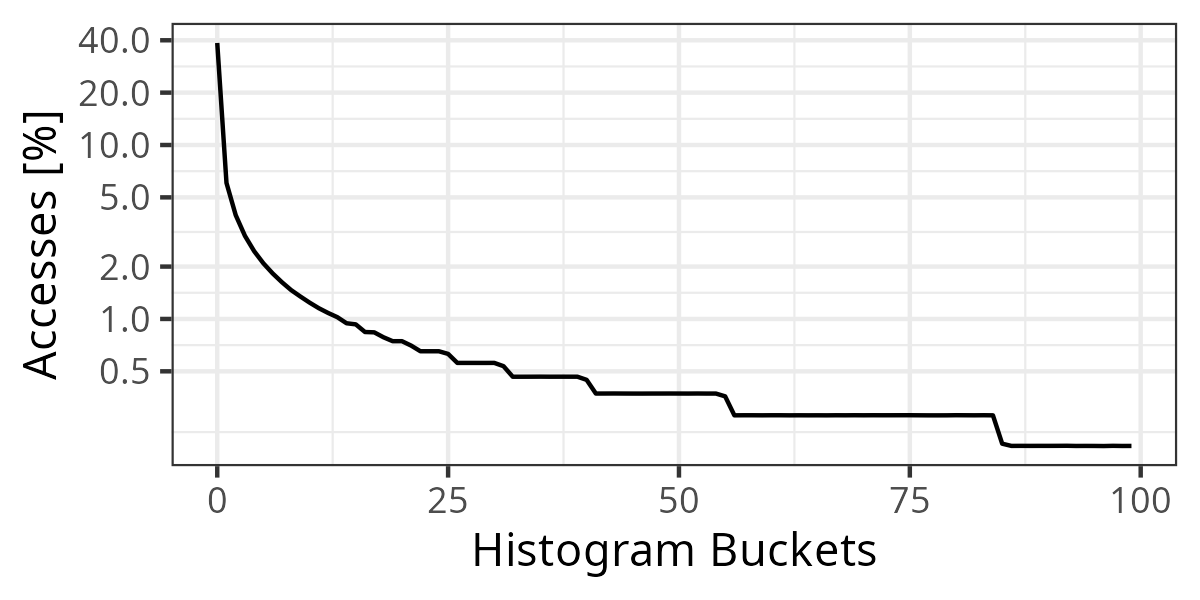
\includegraphics[width=\textwidth]{figures/pmf/marsaglia.png}
        \caption{Condensed Table Lookup}
    \end{subfigure}
    \hfill
    \begin{subfigure}{0.46\textwidth}
        \centering
        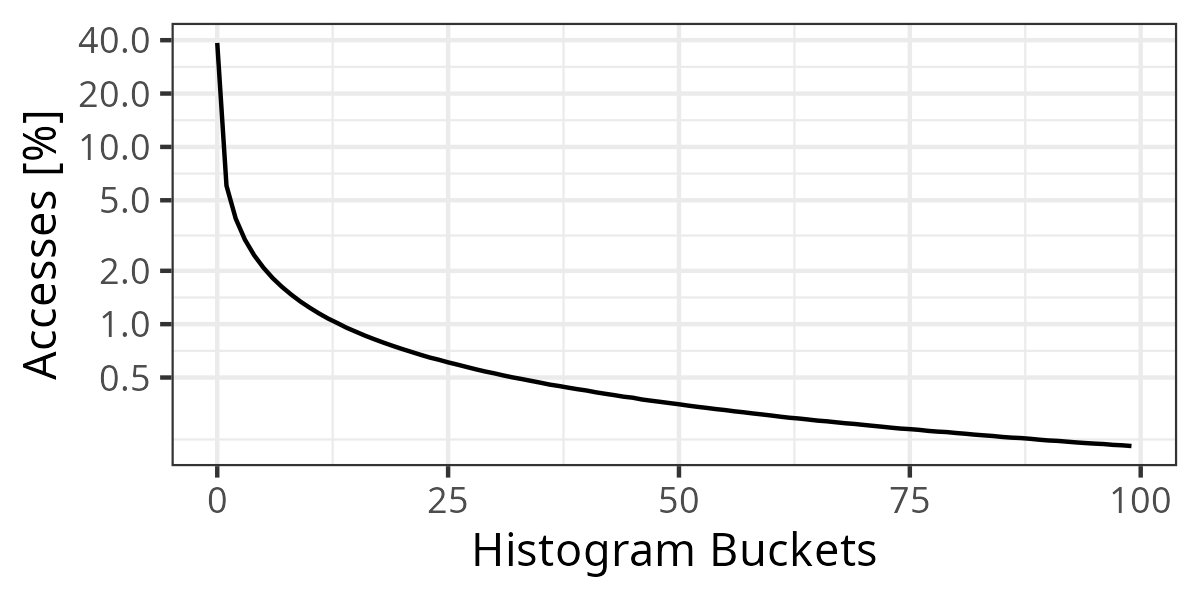
\includegraphics[width=\textwidth]{figures/pmf/rejection.png}
        \caption{Rejection}
    \end{subfigure}

    \label{fig:pmf-graphs}
\end{figure}

\paragraph{Log-scaled graphs}These graphs allows for identifaction of systematic biases in data generation (as explained in Chapter \ref{chapter:background}). The y-axis represents the \textit{counts} and the x-axis the 
\textit{histogram entries} (or "buckets") for all ranks, as shown in figure \ref{fig:log-log}. As was the case before, only FIO and the condensed table lookoup implementations have glaring 
deviations from the expected straight line.

\begin{figure}
    % First row
    \centering
    \begin{subfigure}{0.46\textwidth}
        \centering
        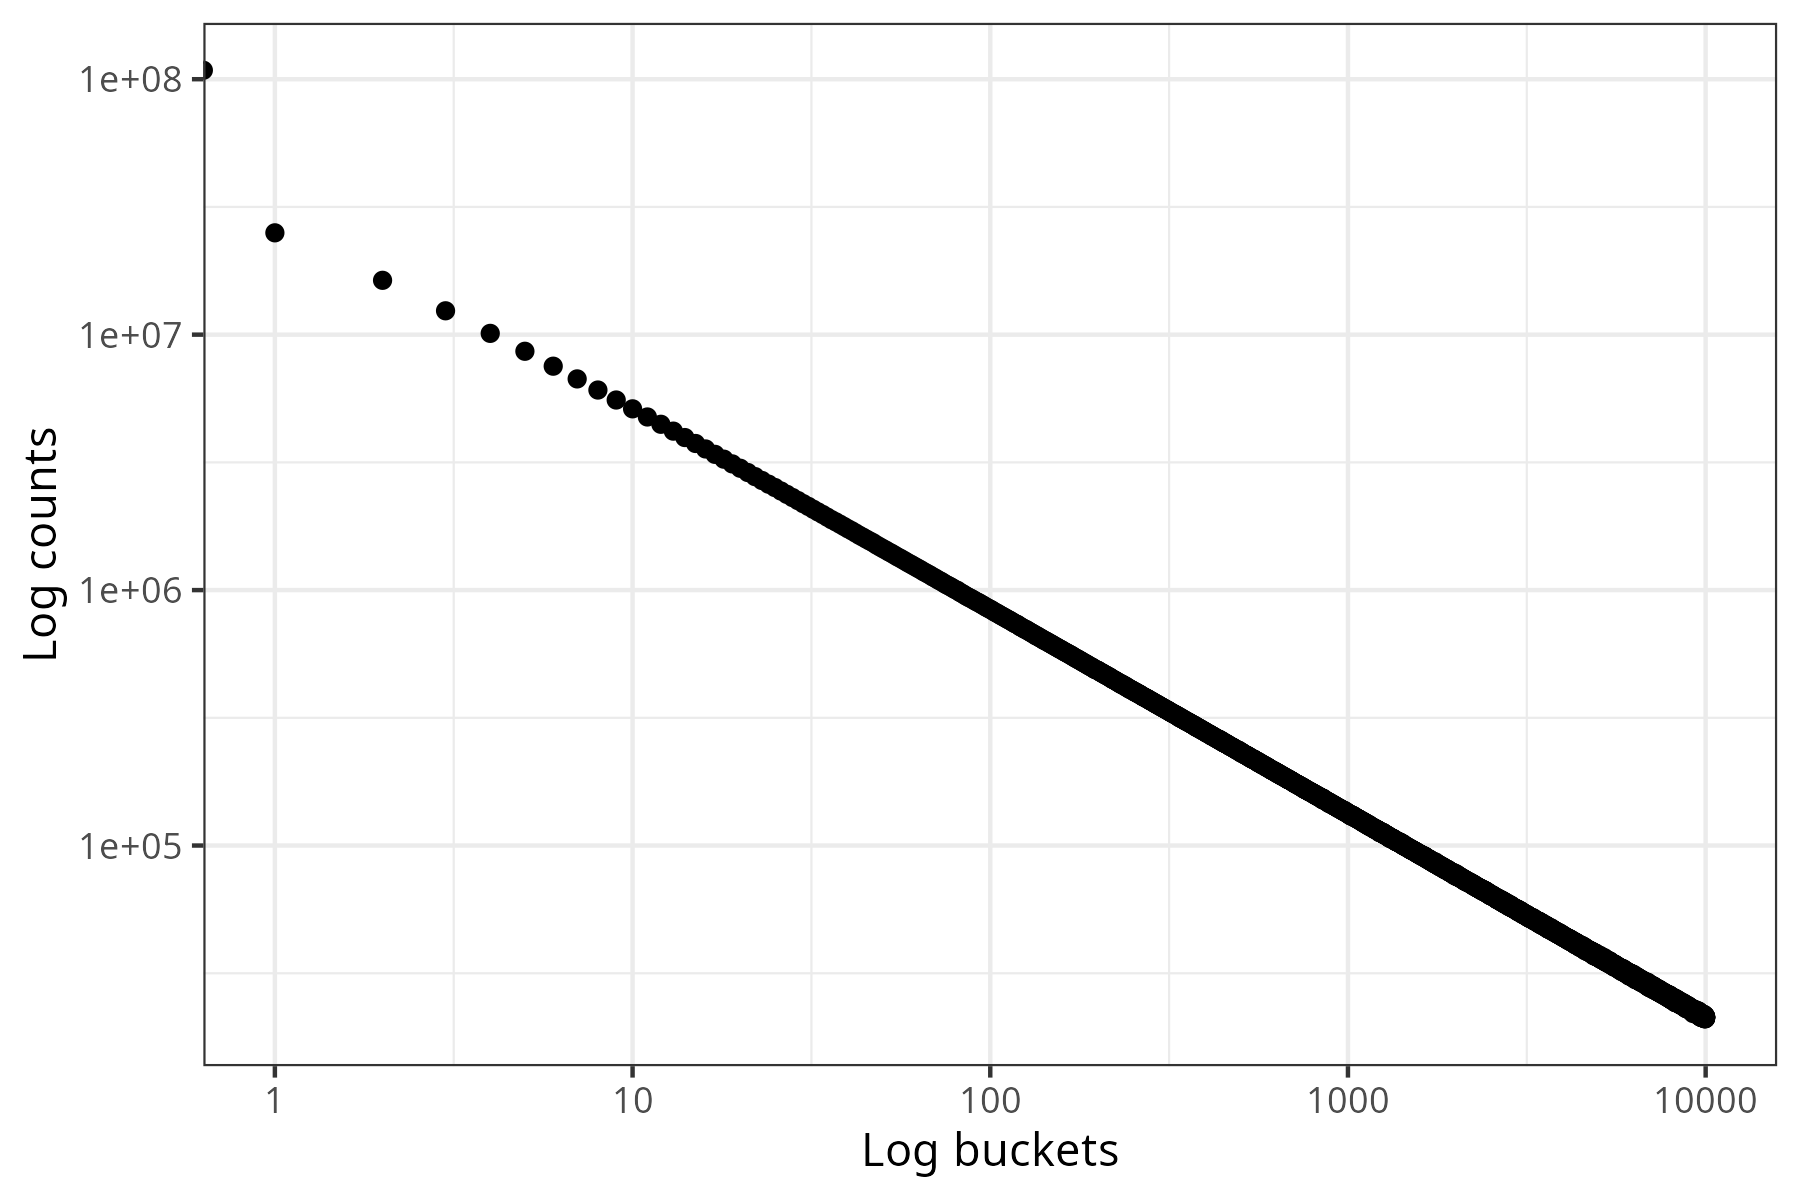
\includegraphics[width=\textwidth]{figures/log-log/apache.png}
        \caption{Rejection-Inversion}
    \end{subfigure}
    \hfill
    \begin{subfigure}{0.46\textwidth}
        \centering
        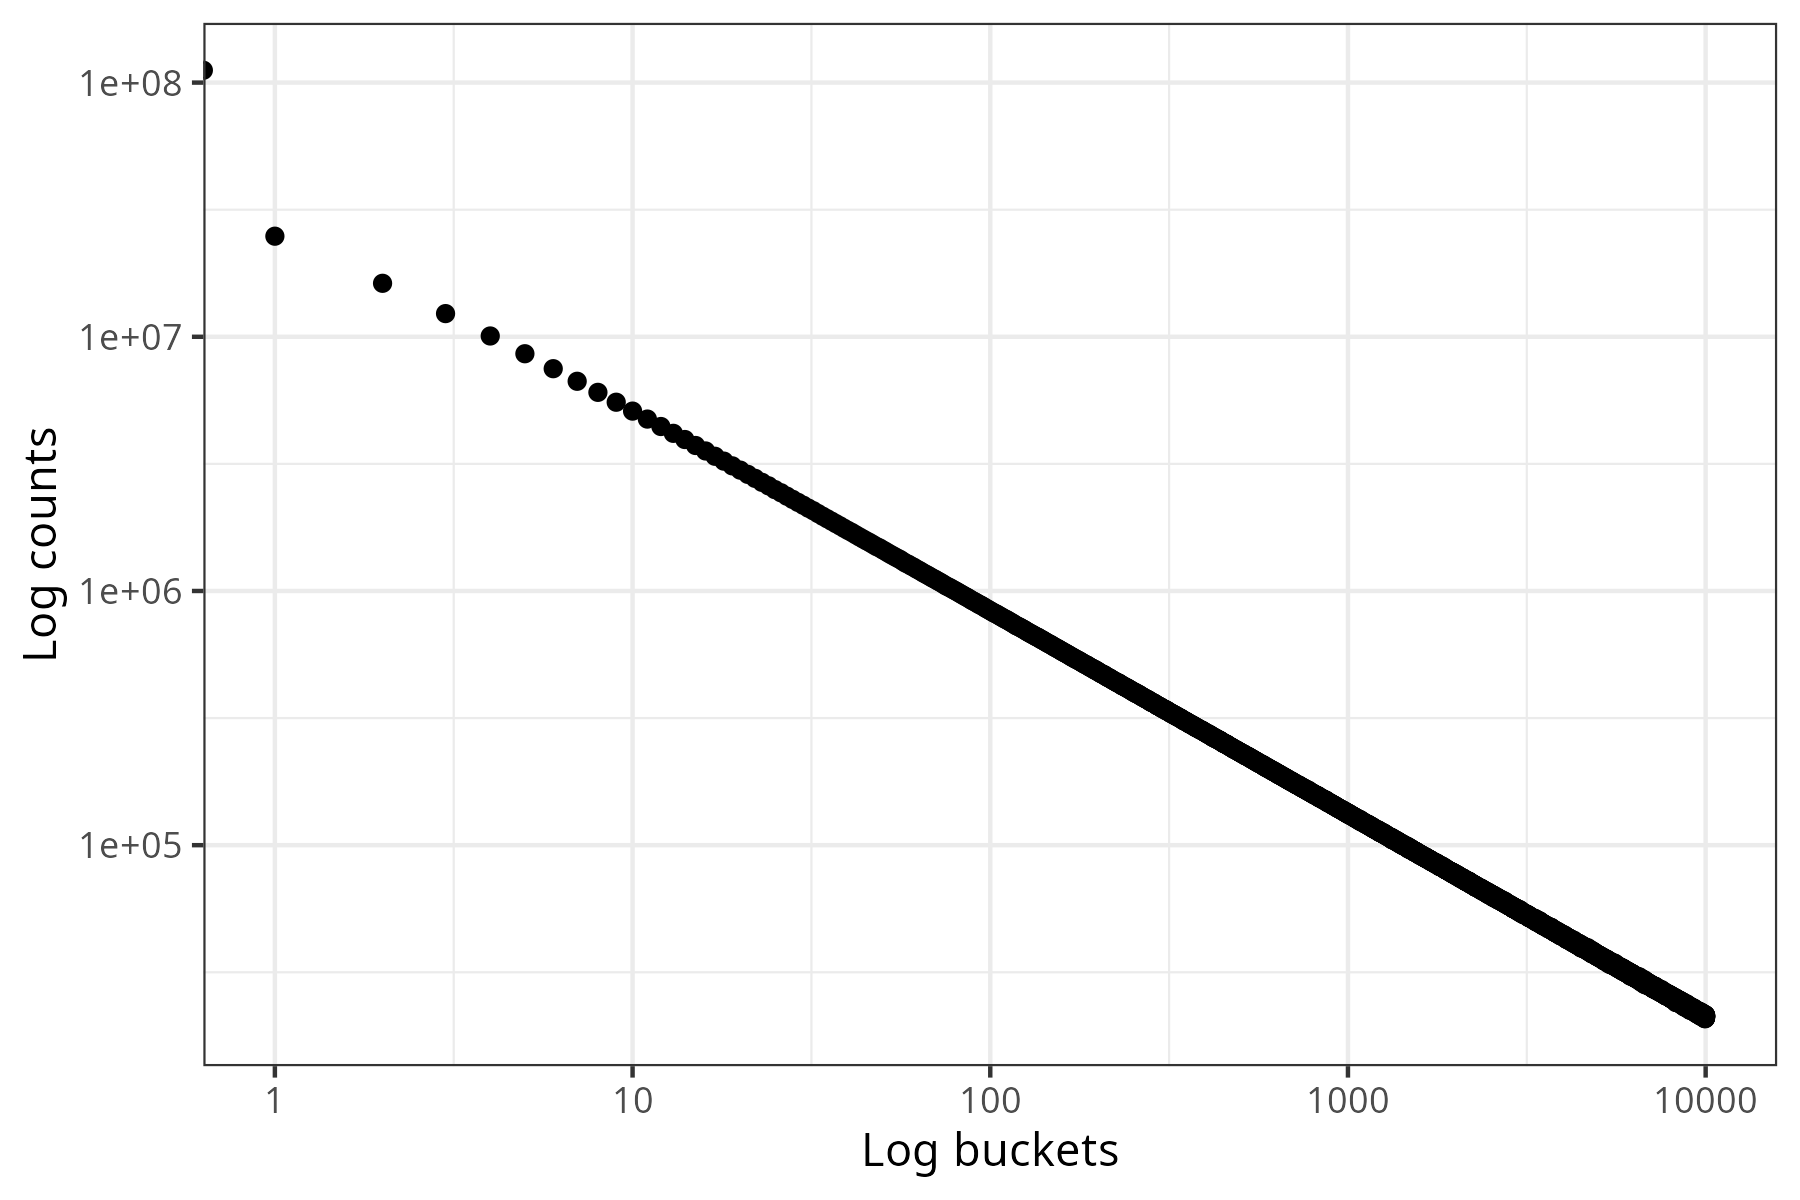
\includegraphics[width=\textwidth]{figures/log-log/ycsb.png}
        \caption{YCSB}
    \end{subfigure}
    
    \vspace{1em}

    % Second row
    \begin{subfigure}{0.46\textwidth}
        \centering
        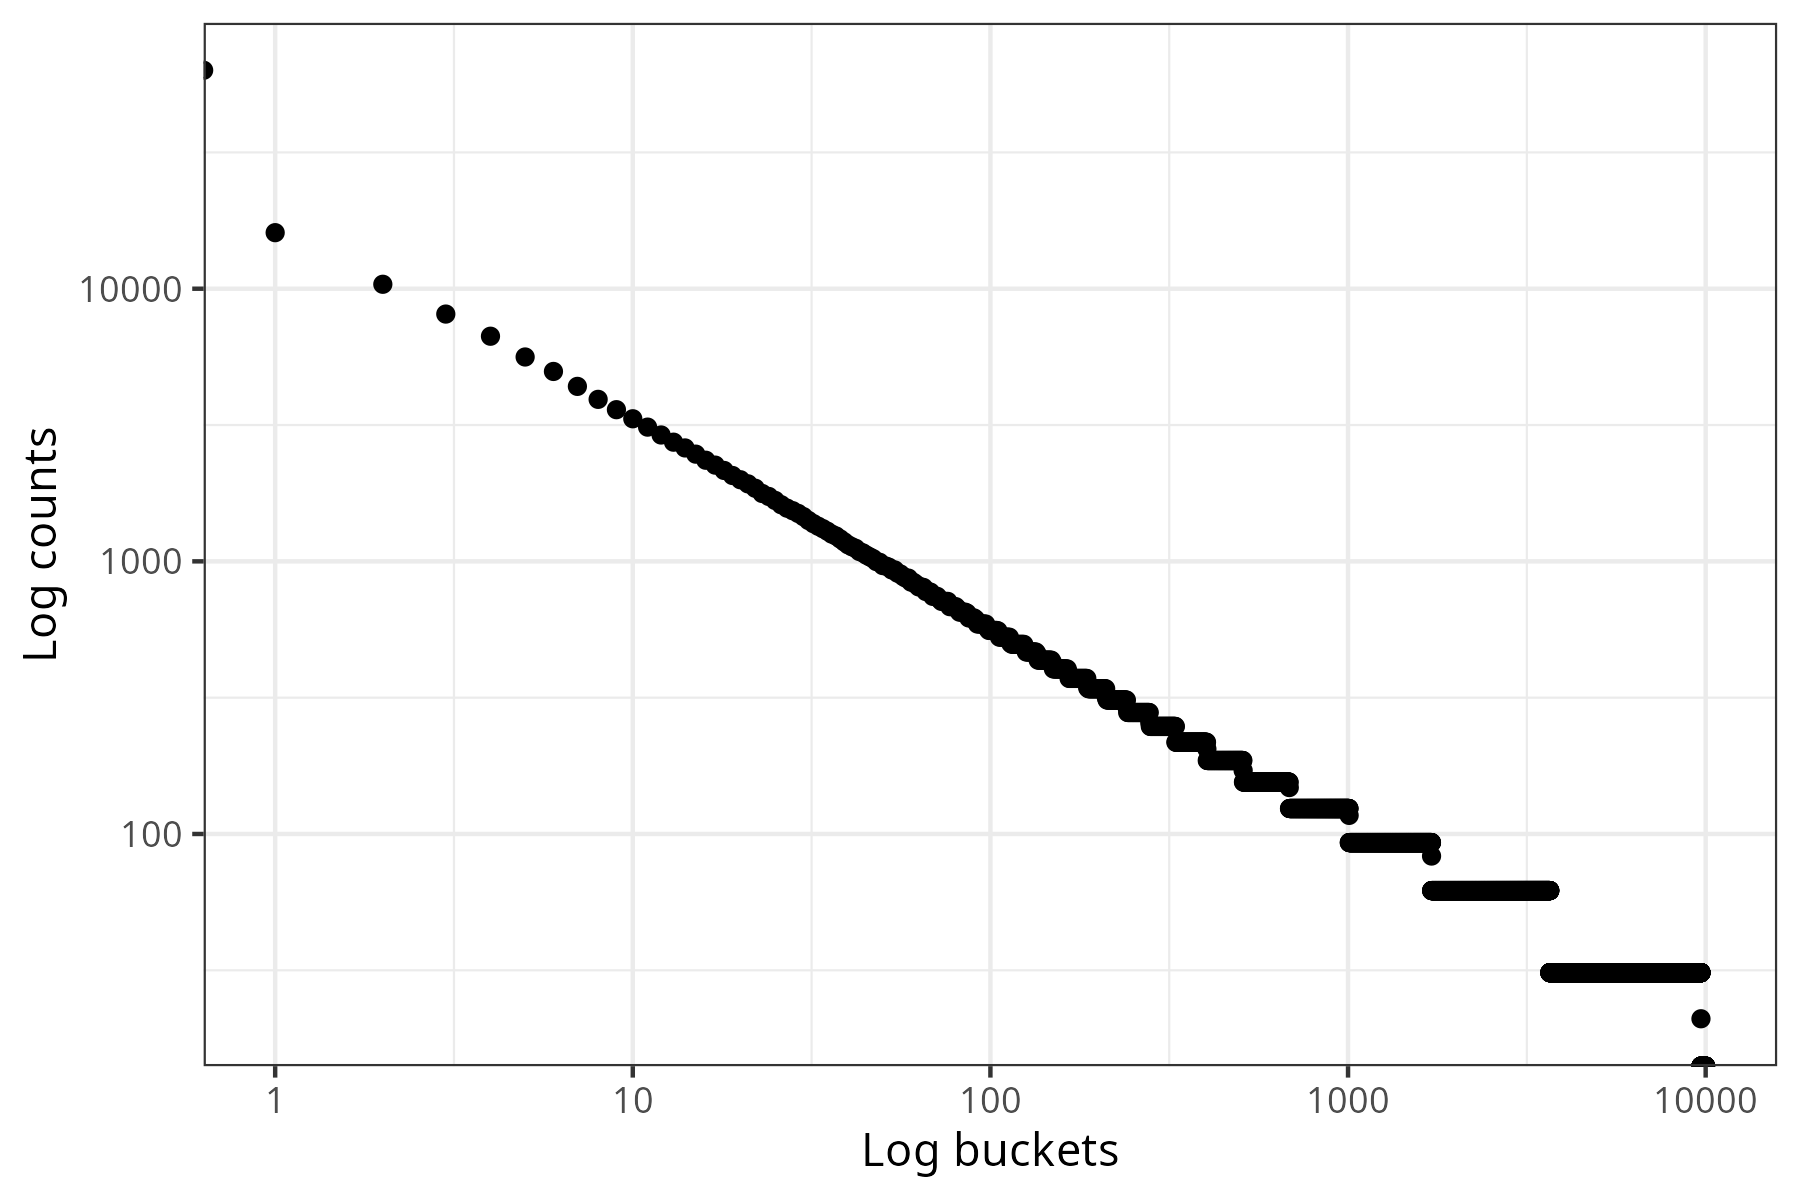
\includegraphics[width=\textwidth]{figures/log-log/fio.png}
        \caption{FIO}
    \end{subfigure}
    \hfill
    \begin{subfigure}{0.46\textwidth}
        \centering
        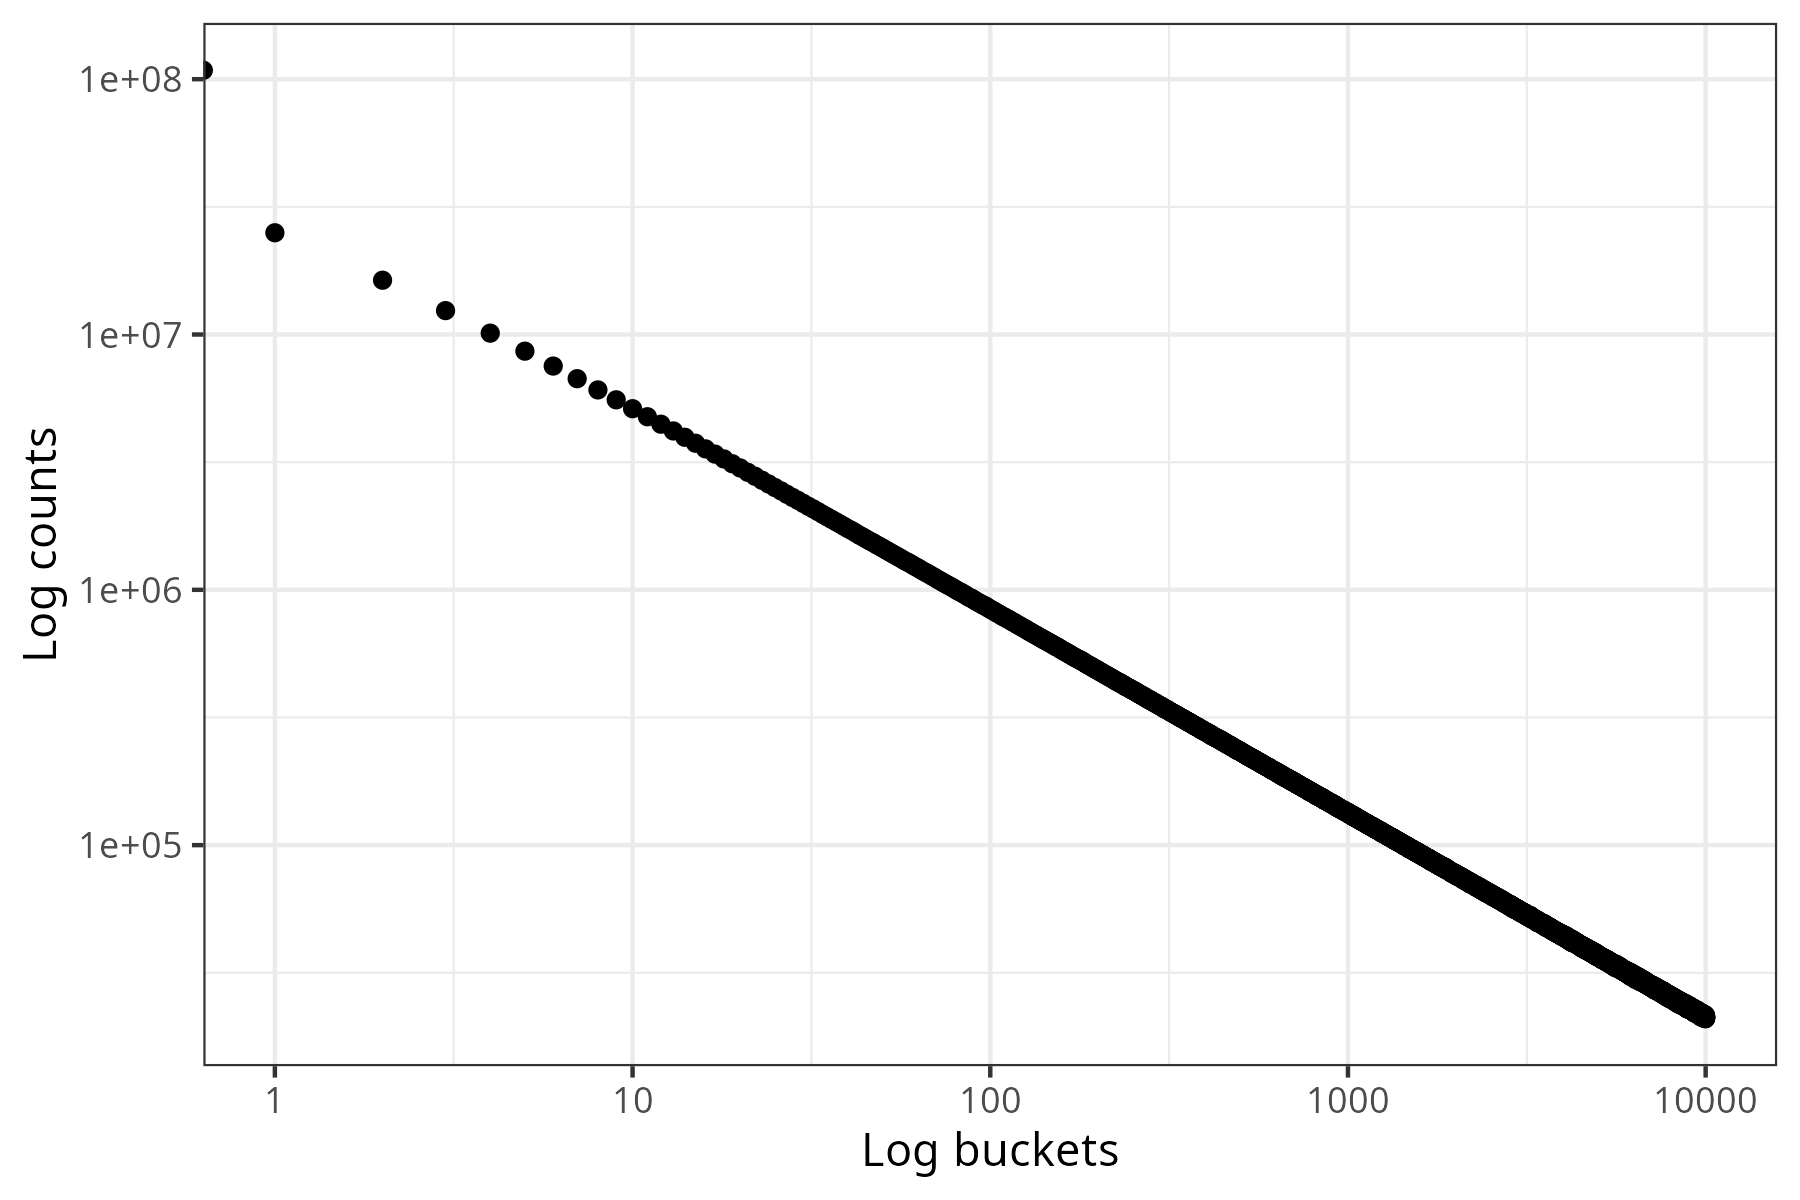
\includegraphics[width=\textwidth]{figures/log-log/sysbench.png}
        \caption{Sysbench}
    \end{subfigure}
    
    \vspace{1em}

    % Third row
    \begin{subfigure}{0.46\textwidth}
        \centering
        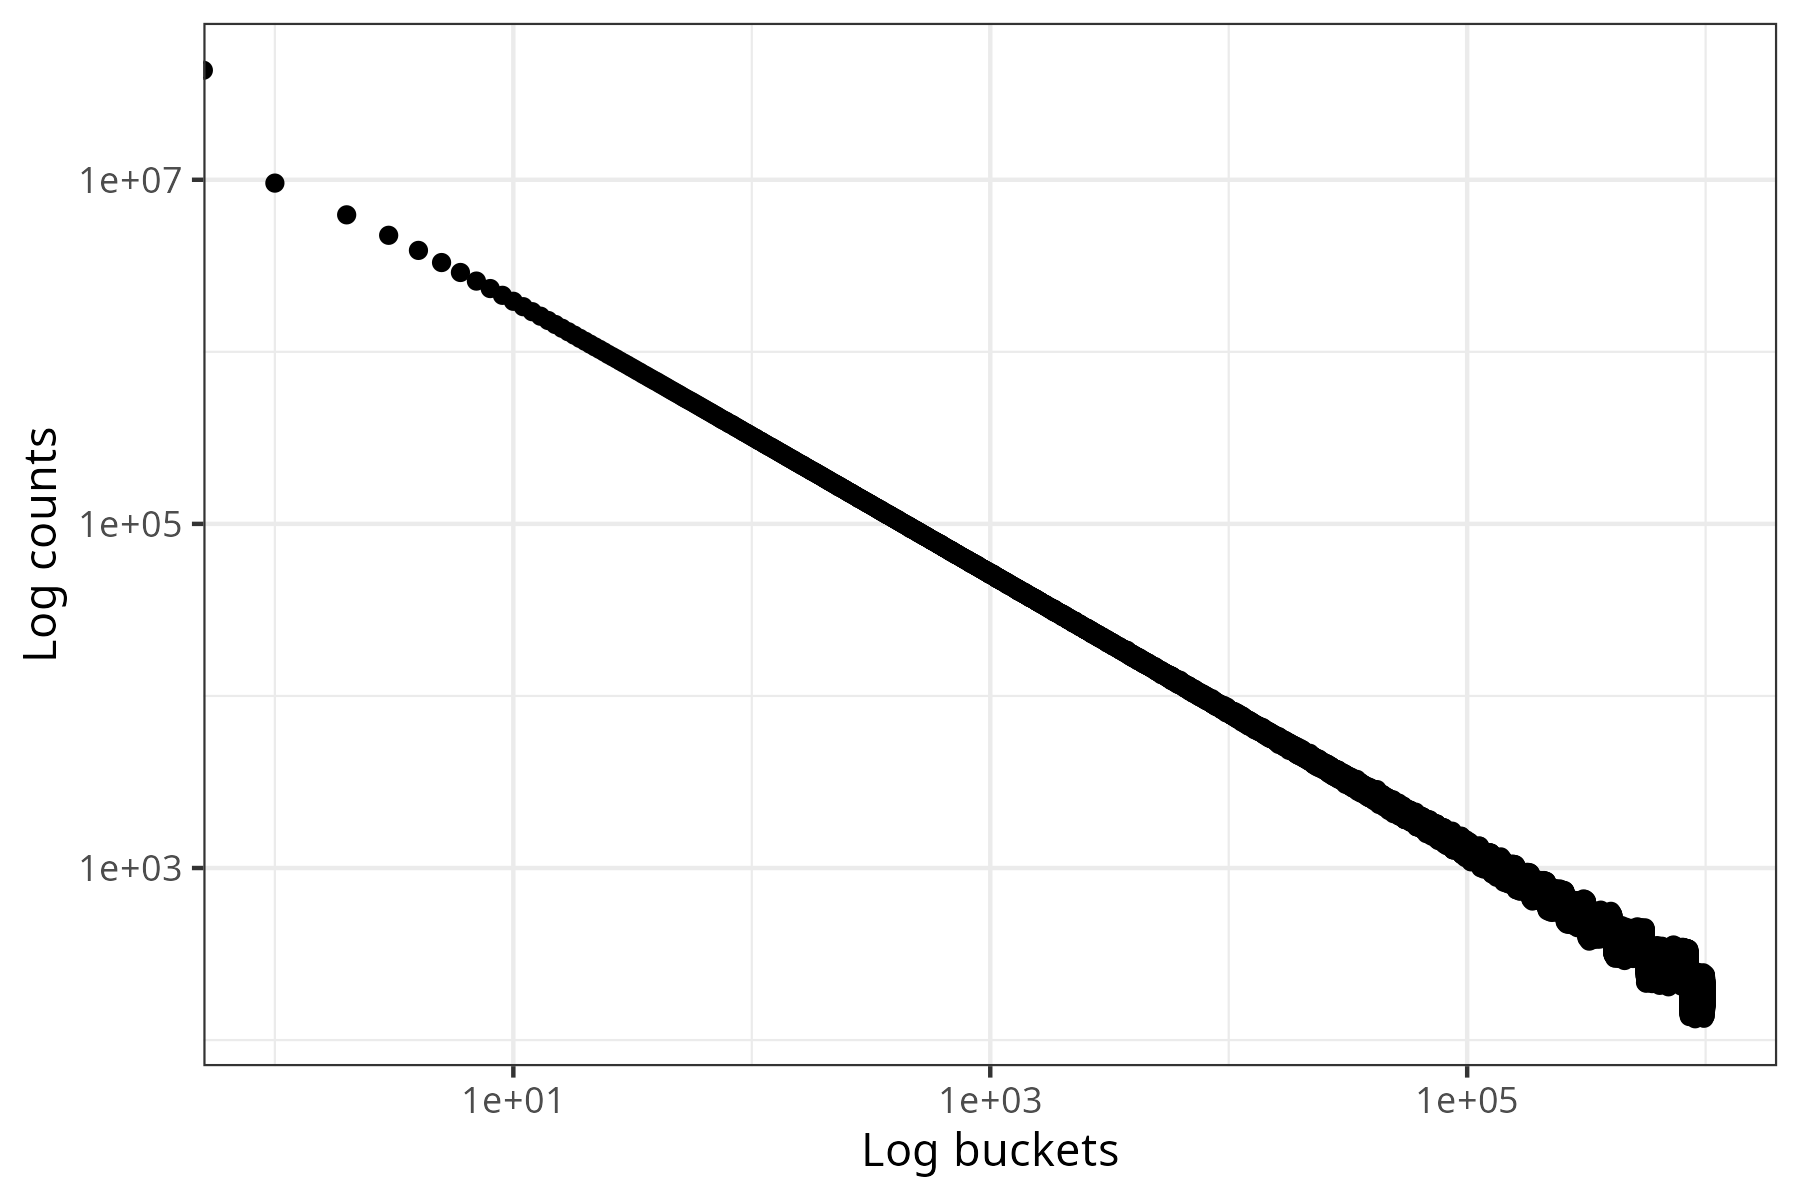
\includegraphics[width=\textwidth]{figures/log-log/marsaglia.png}
        \caption{Condensed Table Lookup}
    \end{subfigure}
    \hfill
    \begin{subfigure}{0.46\textwidth}
        \centering
        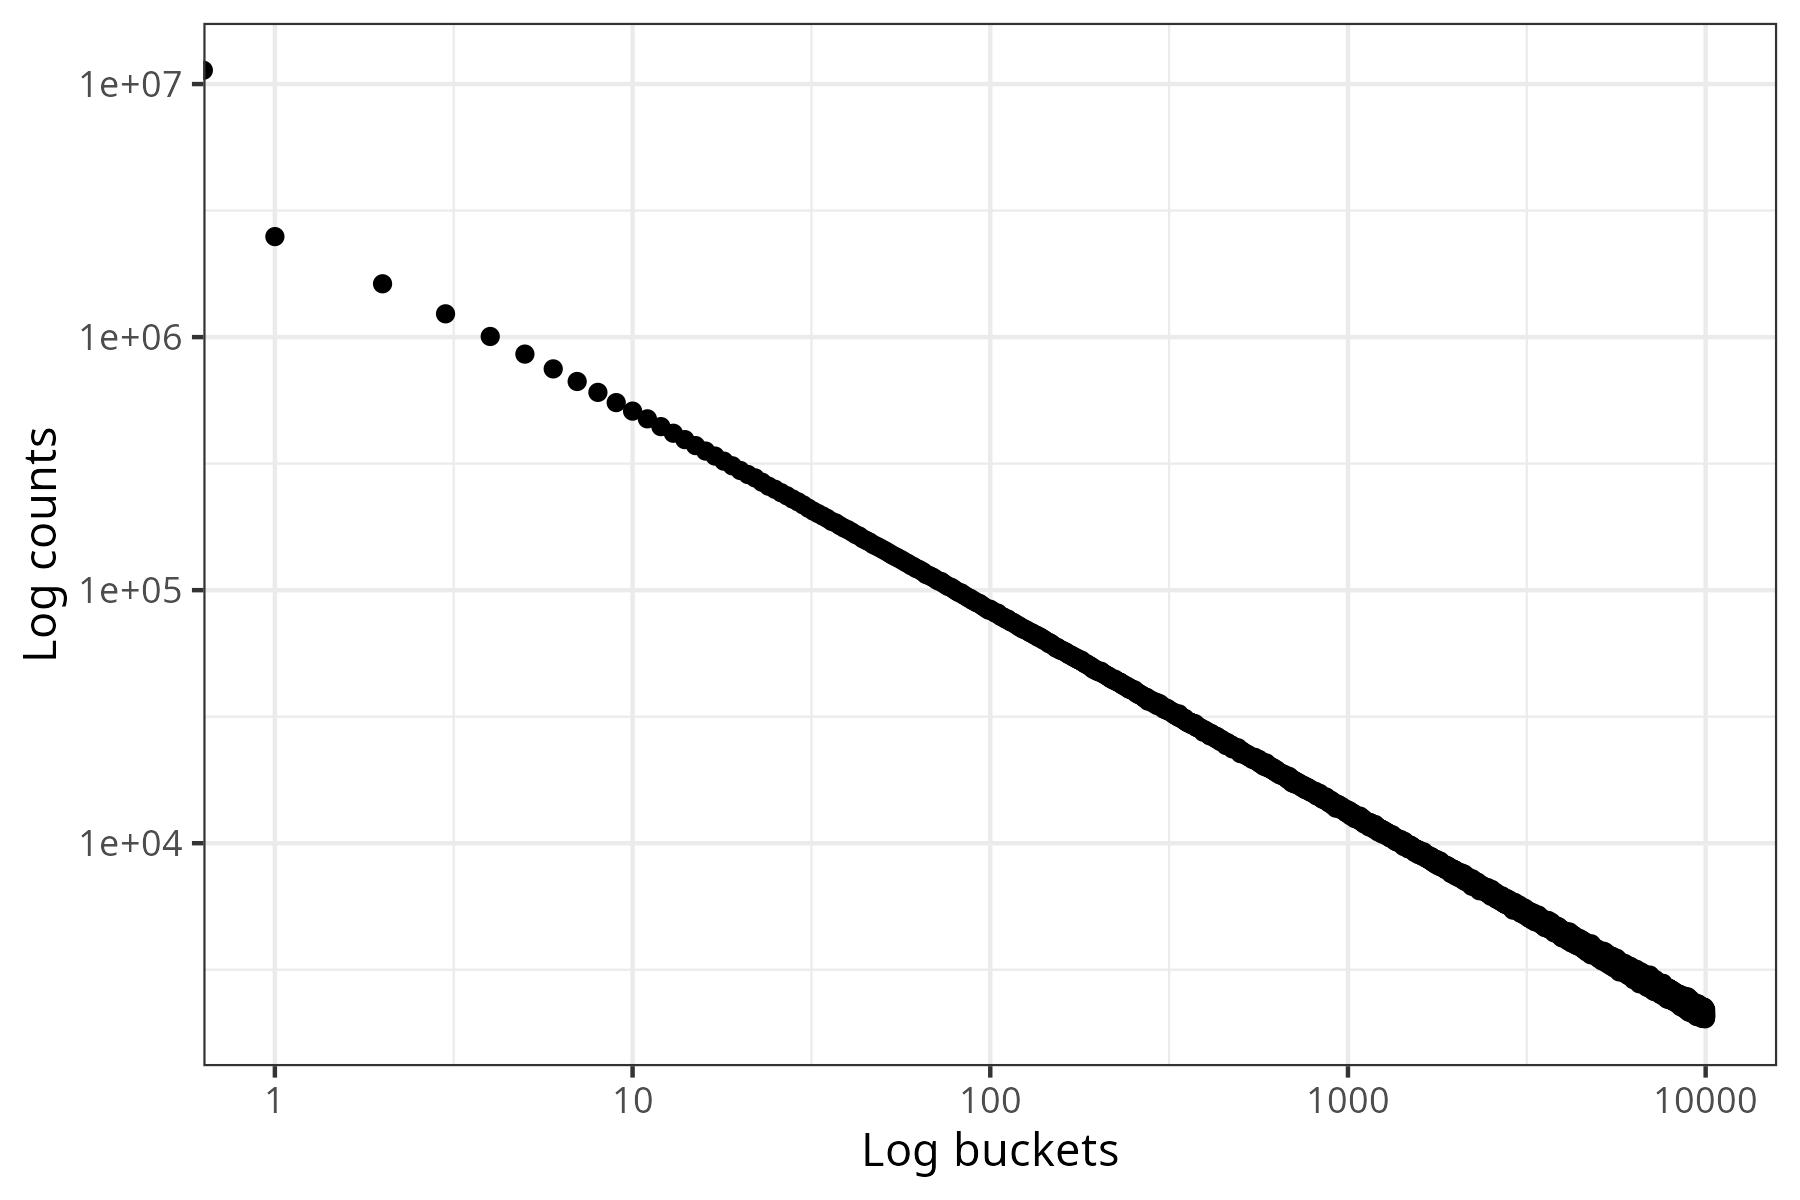
\includegraphics[width=\textwidth]{figures/log-log/rejection.png}
        \caption{Rejection Sampling}
    \end{subfigure}
    
    
    \caption{Log-log plots of the performance of the 6 different variate generators.}
    \label{fig:log-log}
\end{figure}

\paragraph{Frequency Ratio Analysis} 
To further analyse how the accuracy varies within the domain of the distribution, a frequency ratio analysis is conducted. This is done by plotting the ratio of the empirical frequency to the 
theoretical frequency (see Equation \ref{eqt:zm_prob}) against the rank of the variate - $\frac{f_{emp}(k)}{f_{theo}(k)}$, where $k$ denotes the rank.

The graphs in figure \ref{fig:ratio-graphs} show the results for the 6 variate generators.
Clearly, the more problematic distribution is once again FIO, while other implementations fluctuate around 1.0 - the expected value. Observing the equation \ref{eqt:zm_prob} and the graph
of \textit{FIO} in figure \ref{fig:pmf_graphs} dismystifies the problem: The probability stays constants for long stretches of the domain, whereas the real distribution ever so decreases. This
in turn makes the ratio of the empirical to the theoretical frequency increase, before falling off again. 

\begin{figure}[t]
    % First row
    \centering
    \begin{subfigure}{0.46\textwidth}
        \centering
        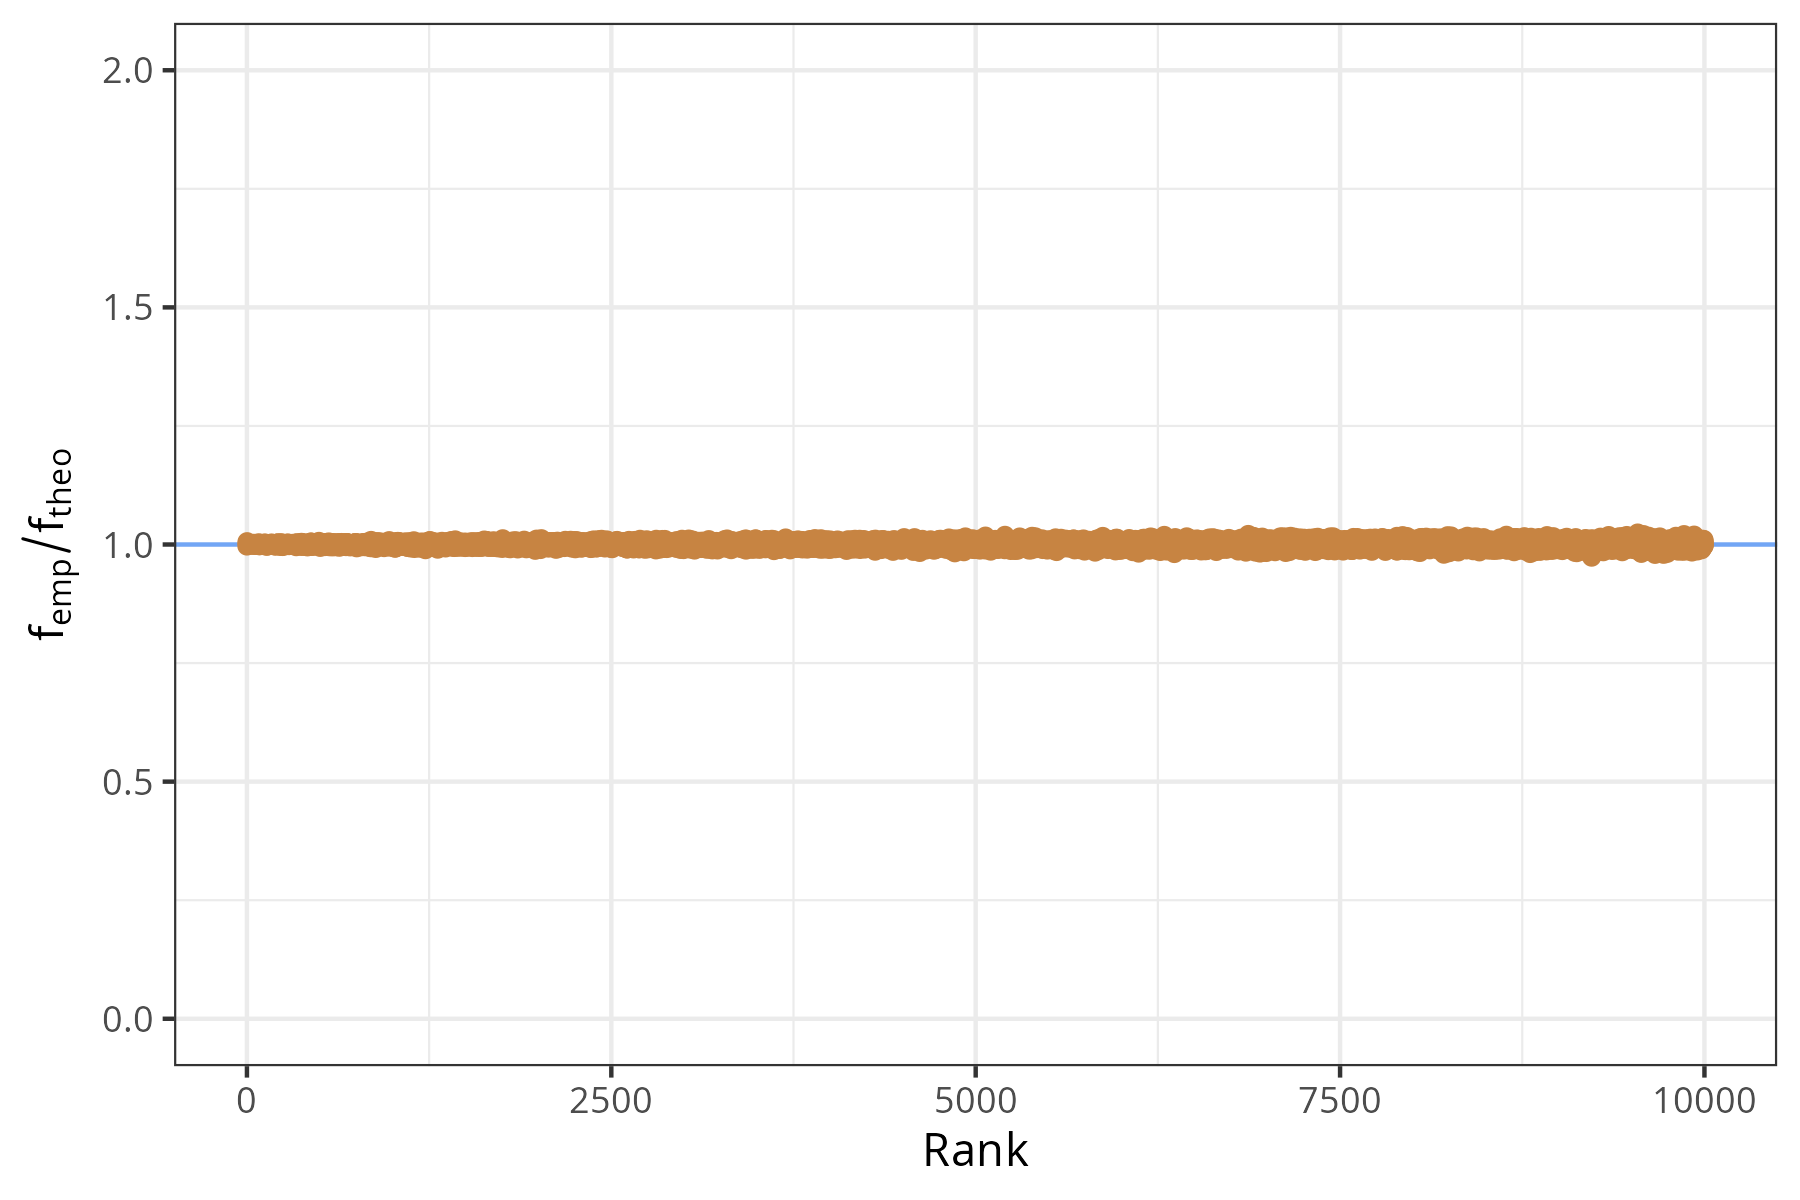
\includegraphics[width=\textwidth]{figures/ratio/apache.png}
        \caption{Rejection inversion}
    \end{subfigure}
    \hfill
    \begin{subfigure}{0.46\textwidth}
        \centering
        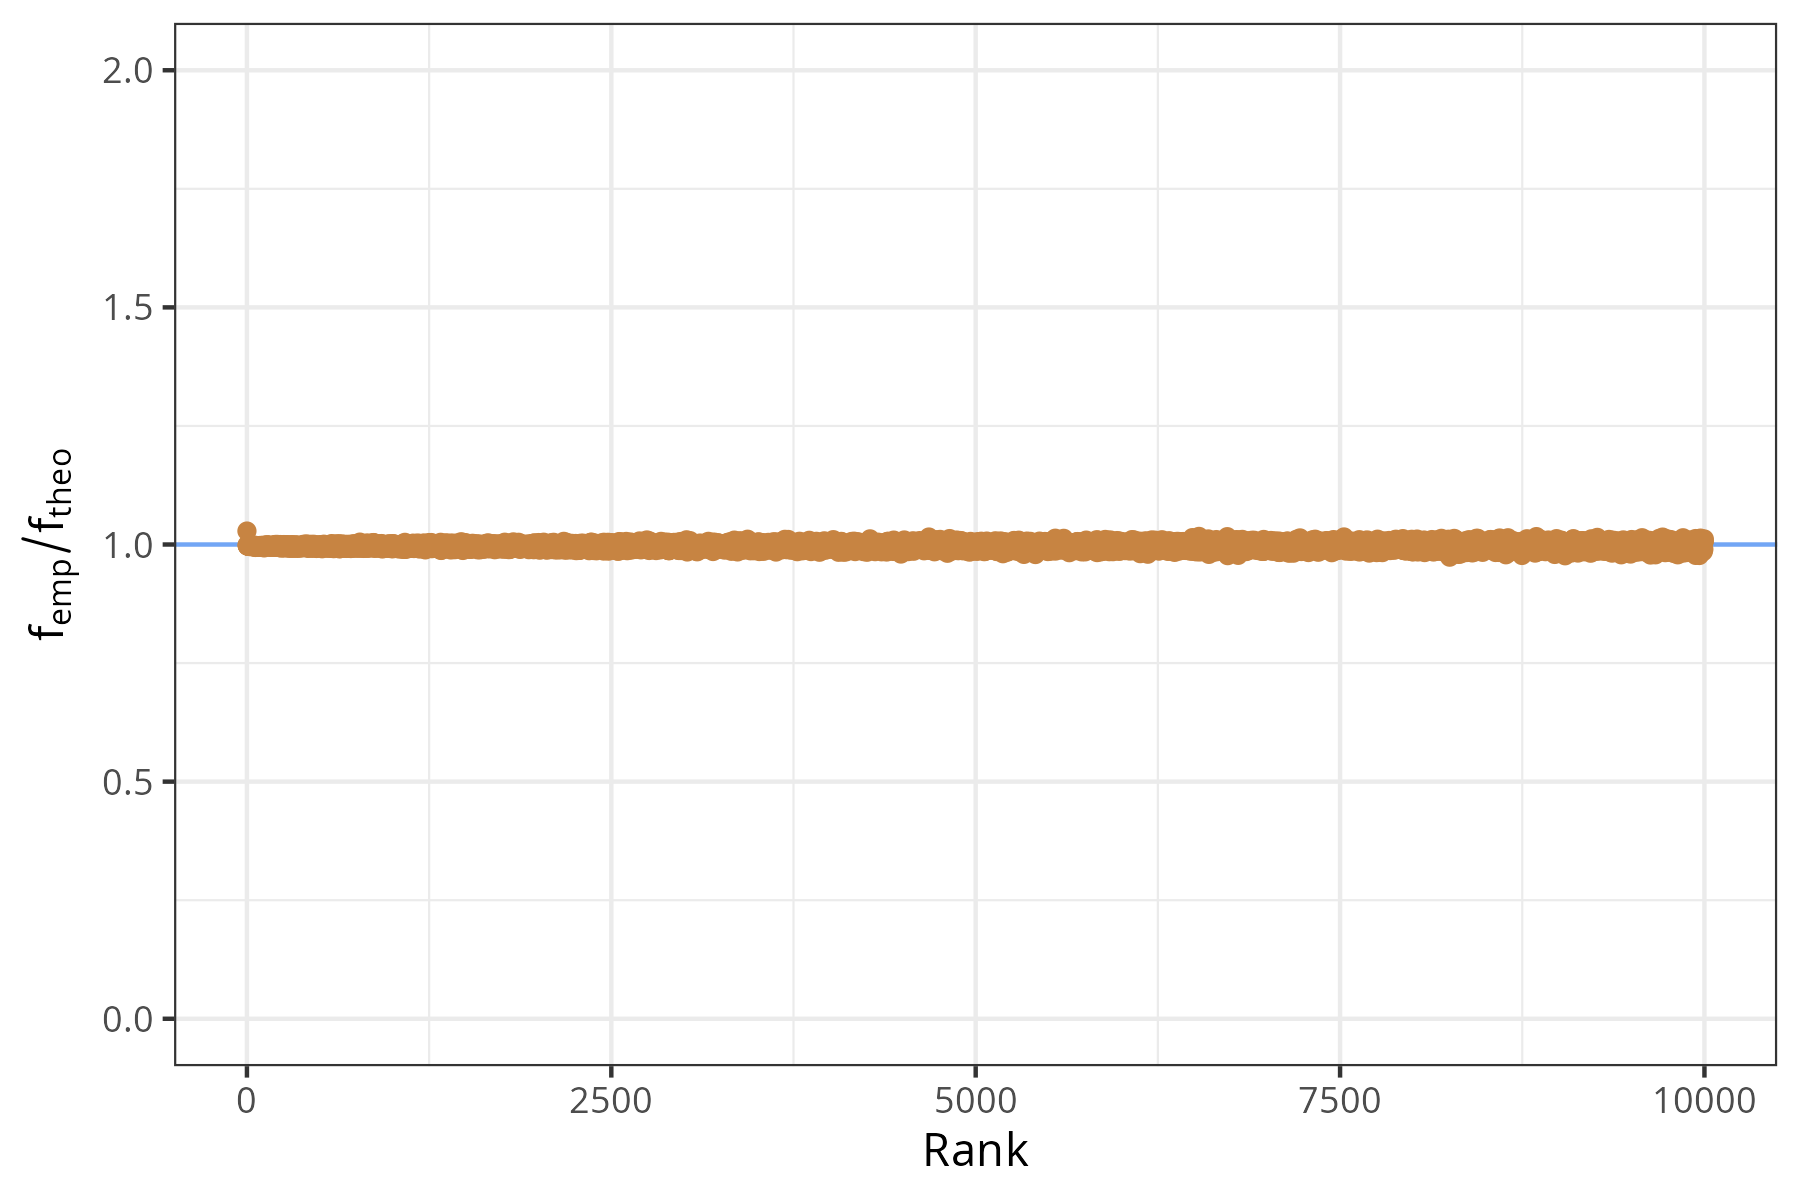
\includegraphics[width=\textwidth]{figures/ratio/ycsb.png}
        \caption{YCSB}
    \end{subfigure}
    
    \vspace{1em} % Space between rows
    
    % Second row
    \begin{subfigure}{0.46\textwidth}
        \centering
        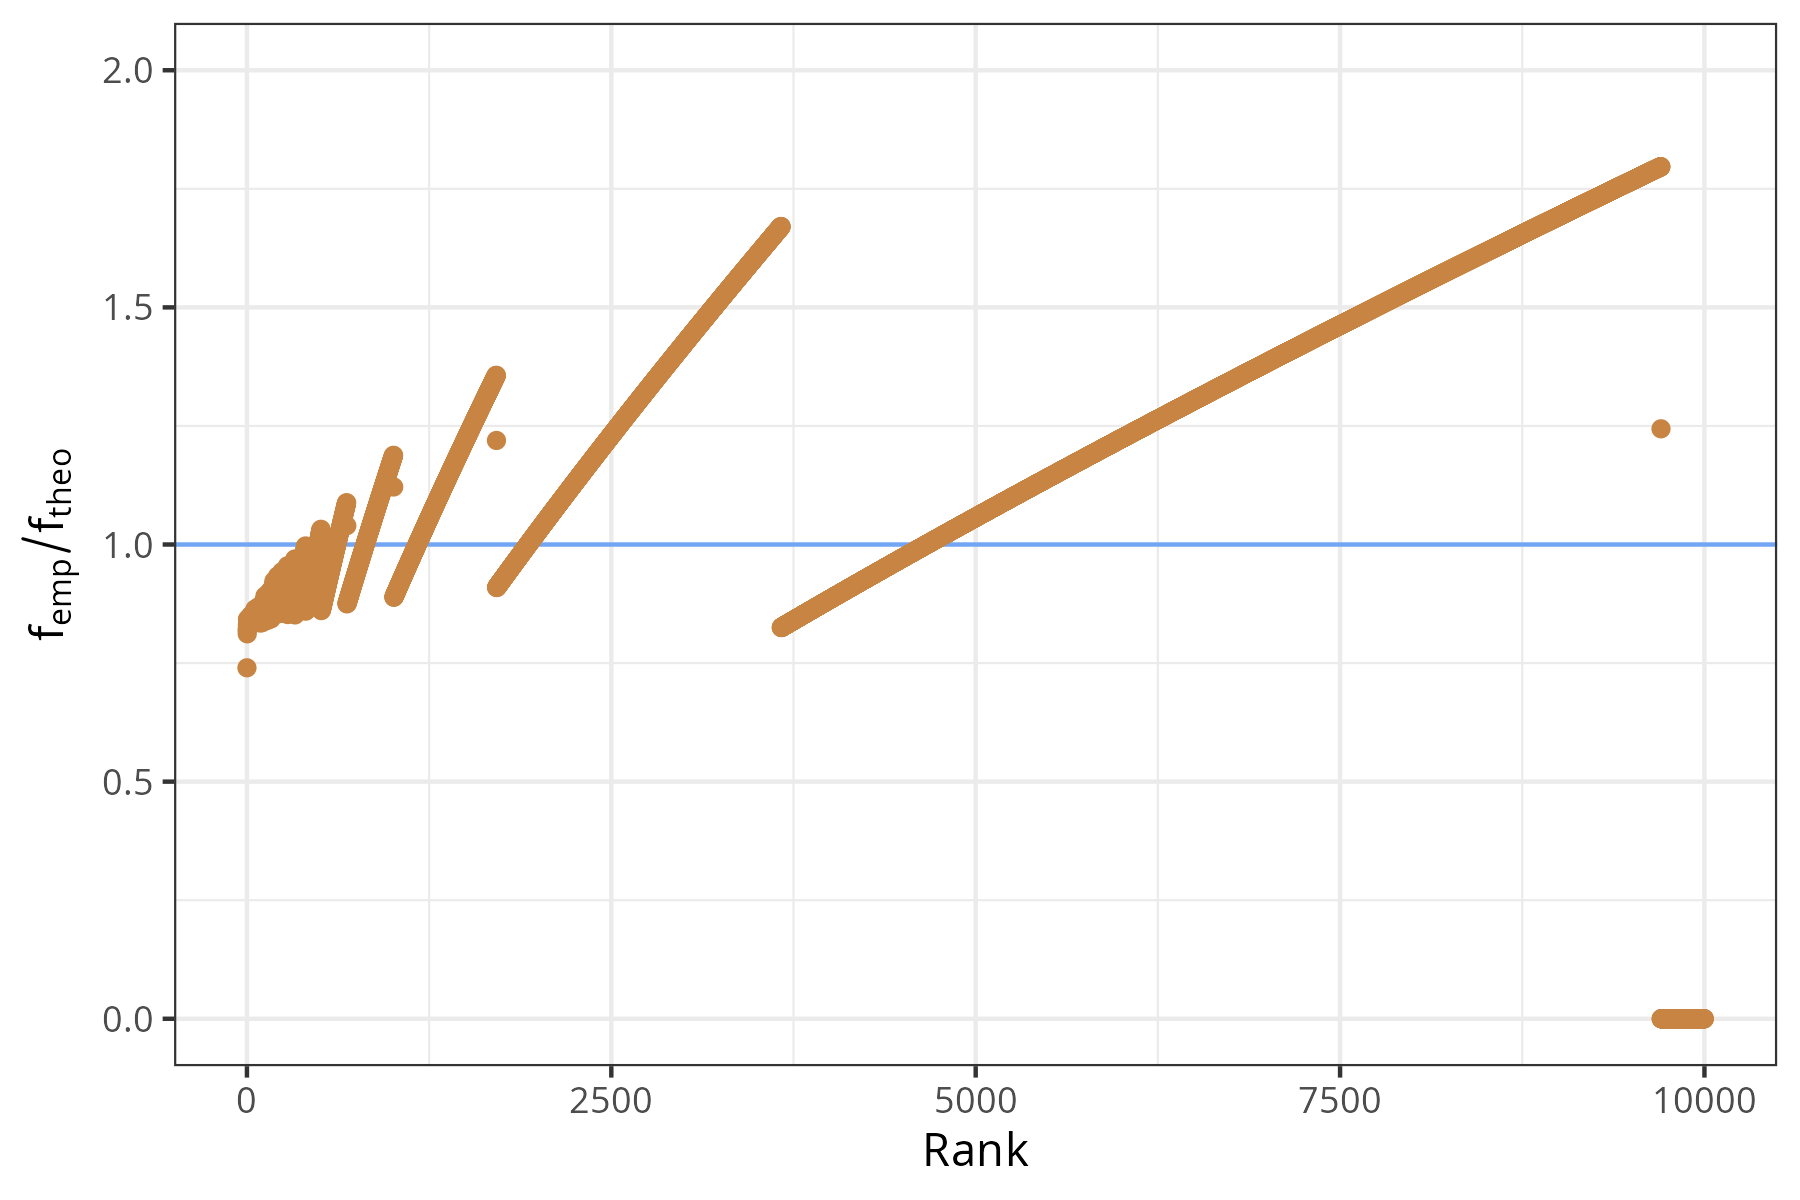
\includegraphics[width=\textwidth]{figures/ratio/fio.png}
        \caption{FIO}
    \end{subfigure}
    \hfill
    \begin{subfigure}{0.46\textwidth}
        \centering
        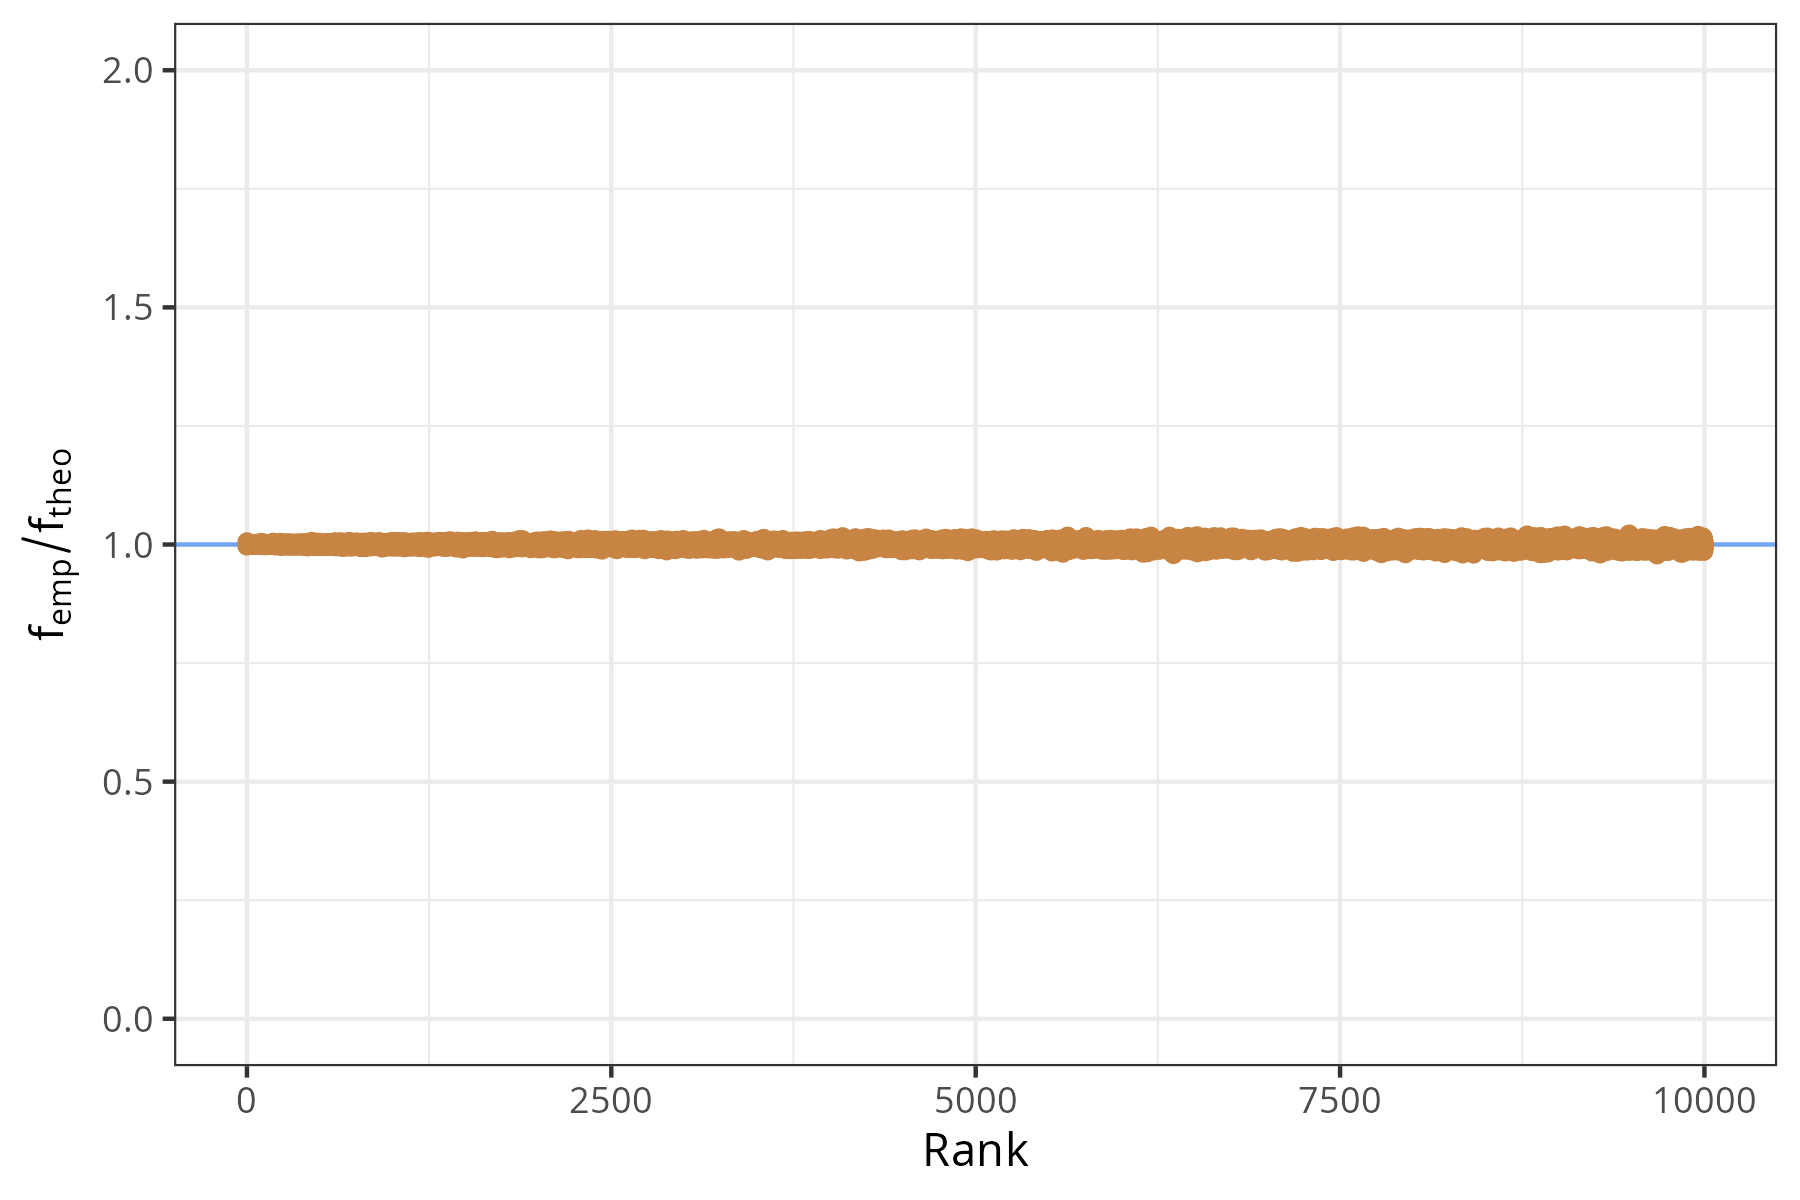
\includegraphics[width=\textwidth]{figures/ratio/sysbench.png}
        \caption{Sysbench}
    \end{subfigure}

    \vspace{1em} % Space between rows
    
    % Third row
    \begin{subfigure}{0.46\textwidth}
        \centering
        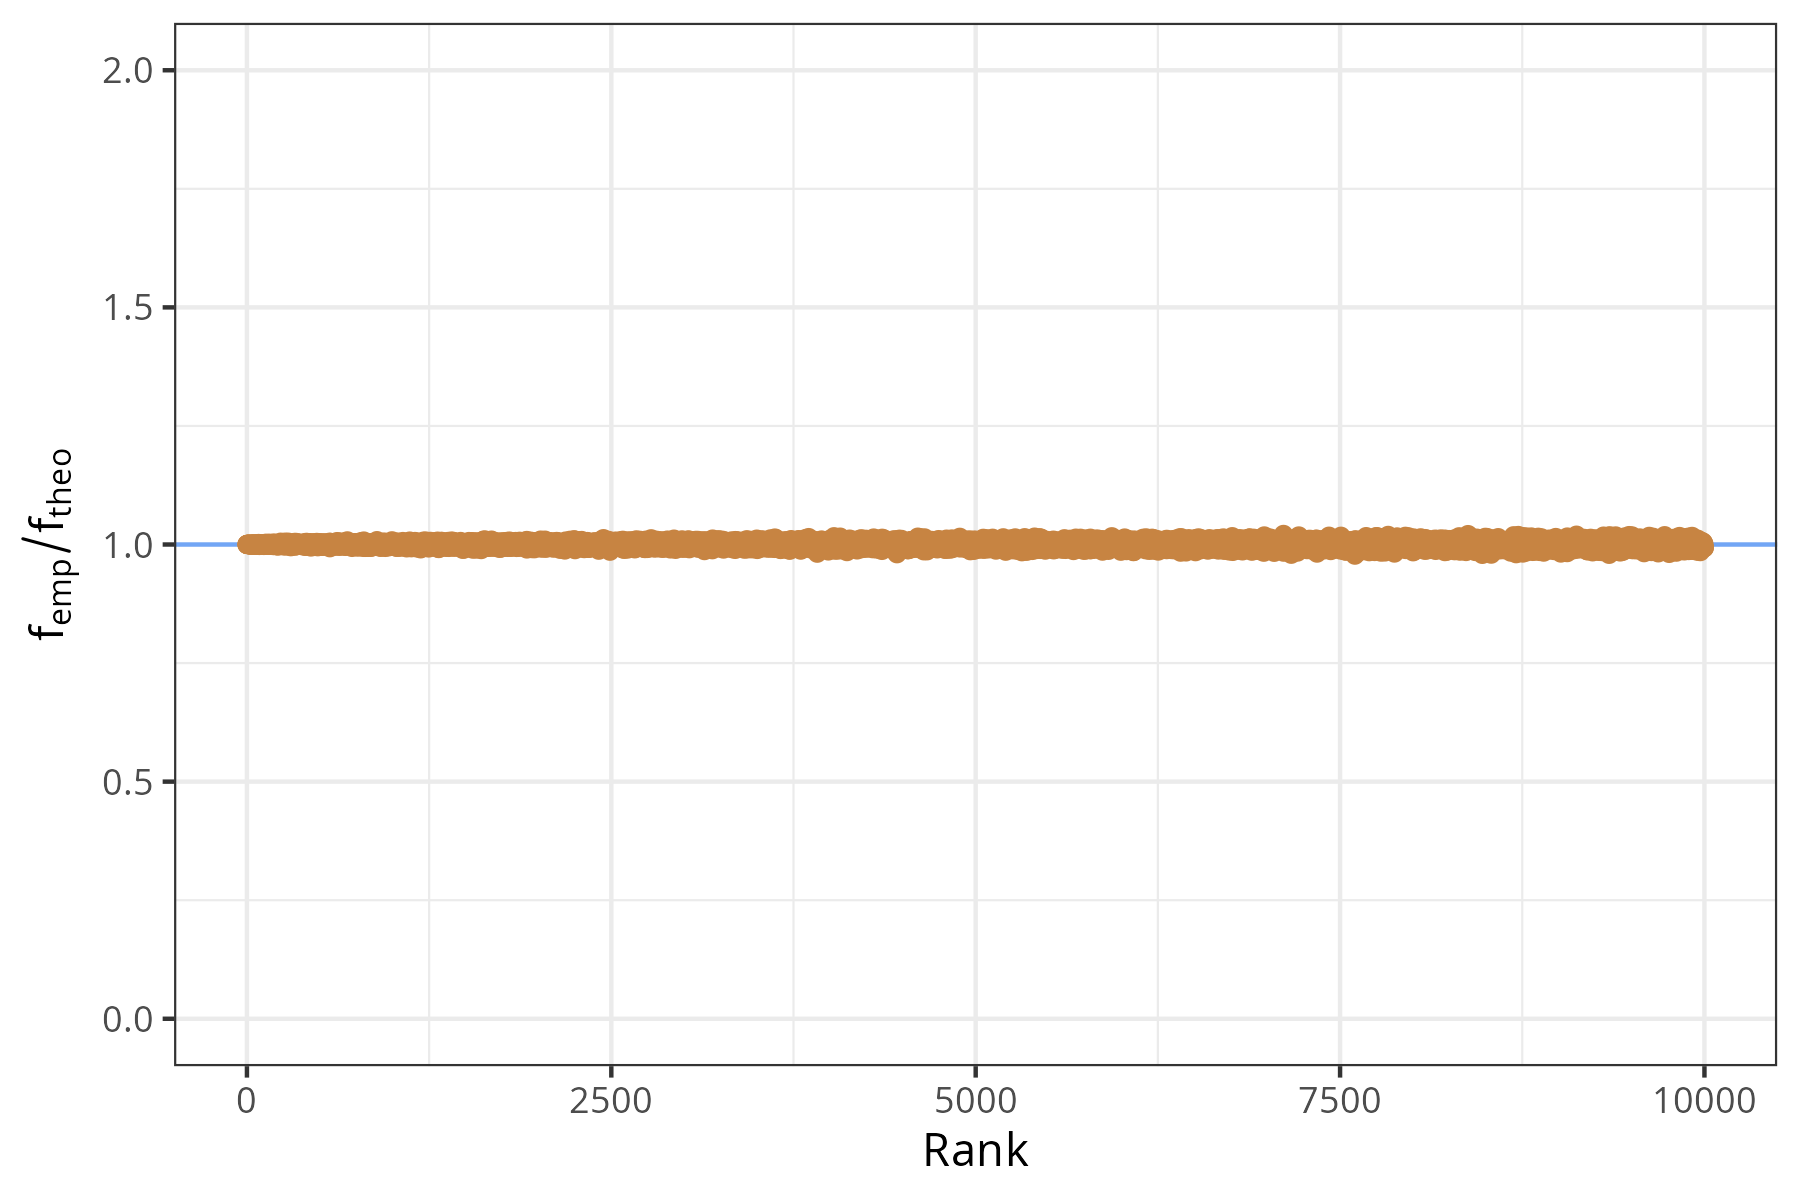
\includegraphics[width=\textwidth]{figures/ratio/marsaglia.png}
        \caption{Condensed Table Lookup}
    \end{subfigure}
    \hfill
    \begin{subfigure}{0.46\textwidth}
        \centering
        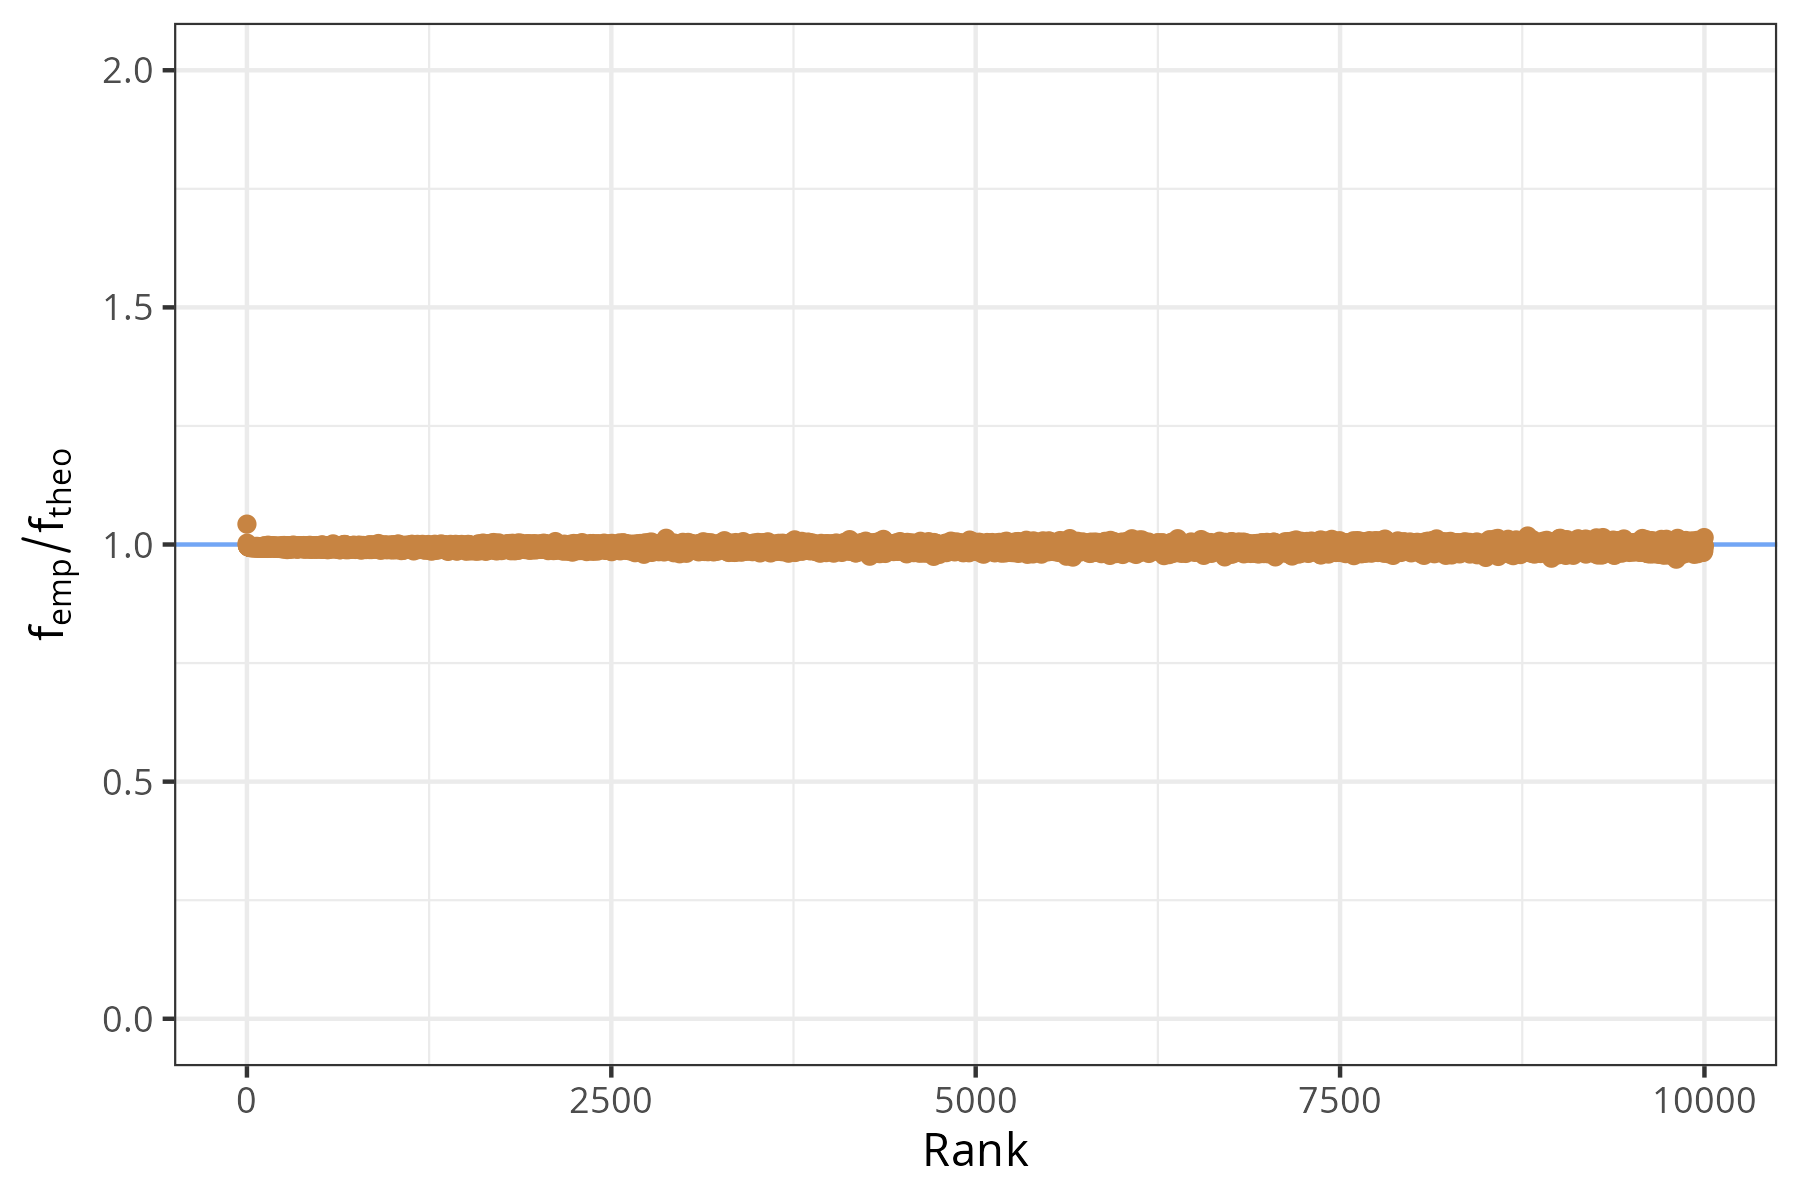
\includegraphics[width=\textwidth]{figures/ratio/rejection.png}
        \caption{Rejection}
    \end{subfigure}

    \caption{All distributions have support size $10^6$ and have $10^9$ samples}
    \label{fig:ratio-graphs}
\end{figure}

\paragraph{Quantitative Criteria} 
First follows the \textbf{Kolmogorov-Smirnov test} in Figure \ref{fig:ks_graphs} and the \textbf{total variation distance} in Figure \ref{fig:tvd-graphs}. From both graphs,
we notice that the FIO implementation is the one that deviates the most from the expected values, while the other implementations are very close to the expected values. Since all but FIO
converge to smaller error values, we can discard the hypothesis that some there are systematic errors and that all implementations are accurate. While there 
is some evidence that moments (such as mean, variance) of self-similar distributions, such as the Zipfian distribution, only very slowly converge to their theoretical values in a sampling environment \cite{crovellaSimulationsHeavyTailedWorkloads2000}
, it seems that for the \textit{Rejection Inversion} (Sysbench, AuctionMark), \textit{Rejection} and \textit{approximative} (YCSB, FIO) sampling algorithms, the distributions are very close to the expected values given enough samples. 
The table \ref{tab:accuracy-results} summarizes the results for sample size = $10^9$.

\begin{figure}[t]
    % First row
    \centering
    \begin{subfigure}{0.46\textwidth}
        \centering
        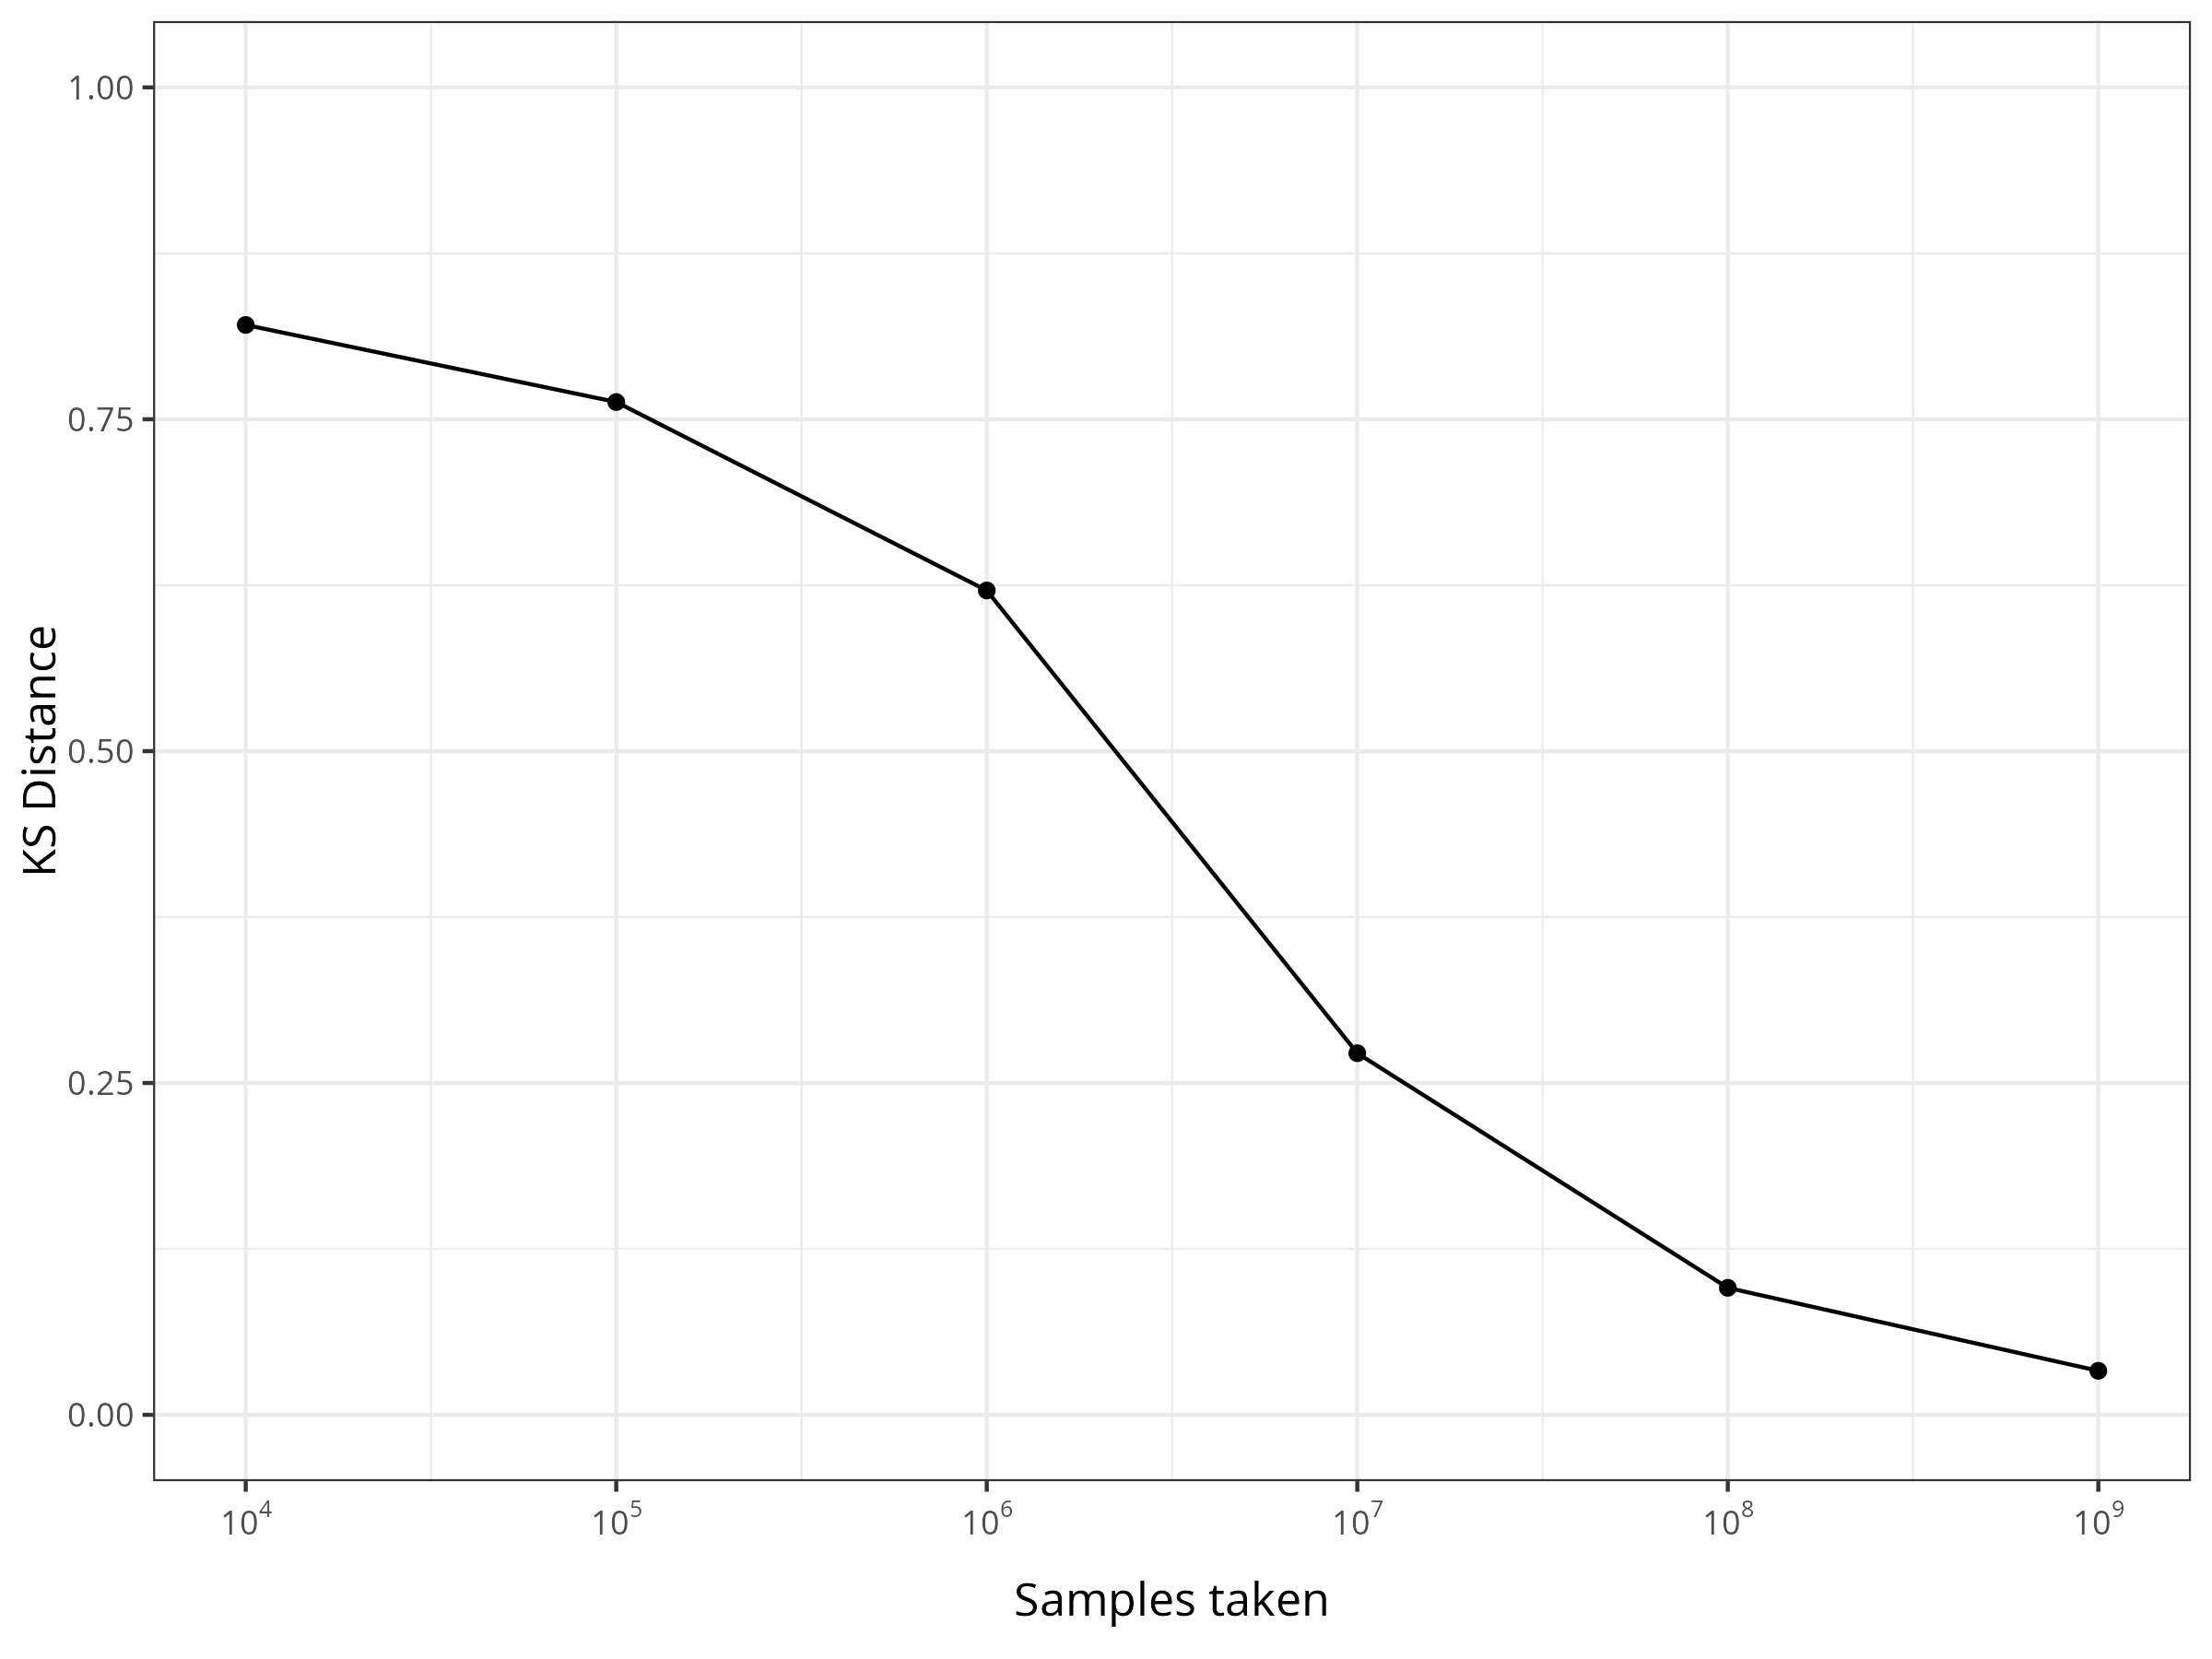
\includegraphics[width=\textwidth]{figures/ks/apache.png}
        \caption{Rejection-Inversion}
    \end{subfigure}
    \hfill
    \begin{subfigure}{0.46\textwidth}
        \centering
        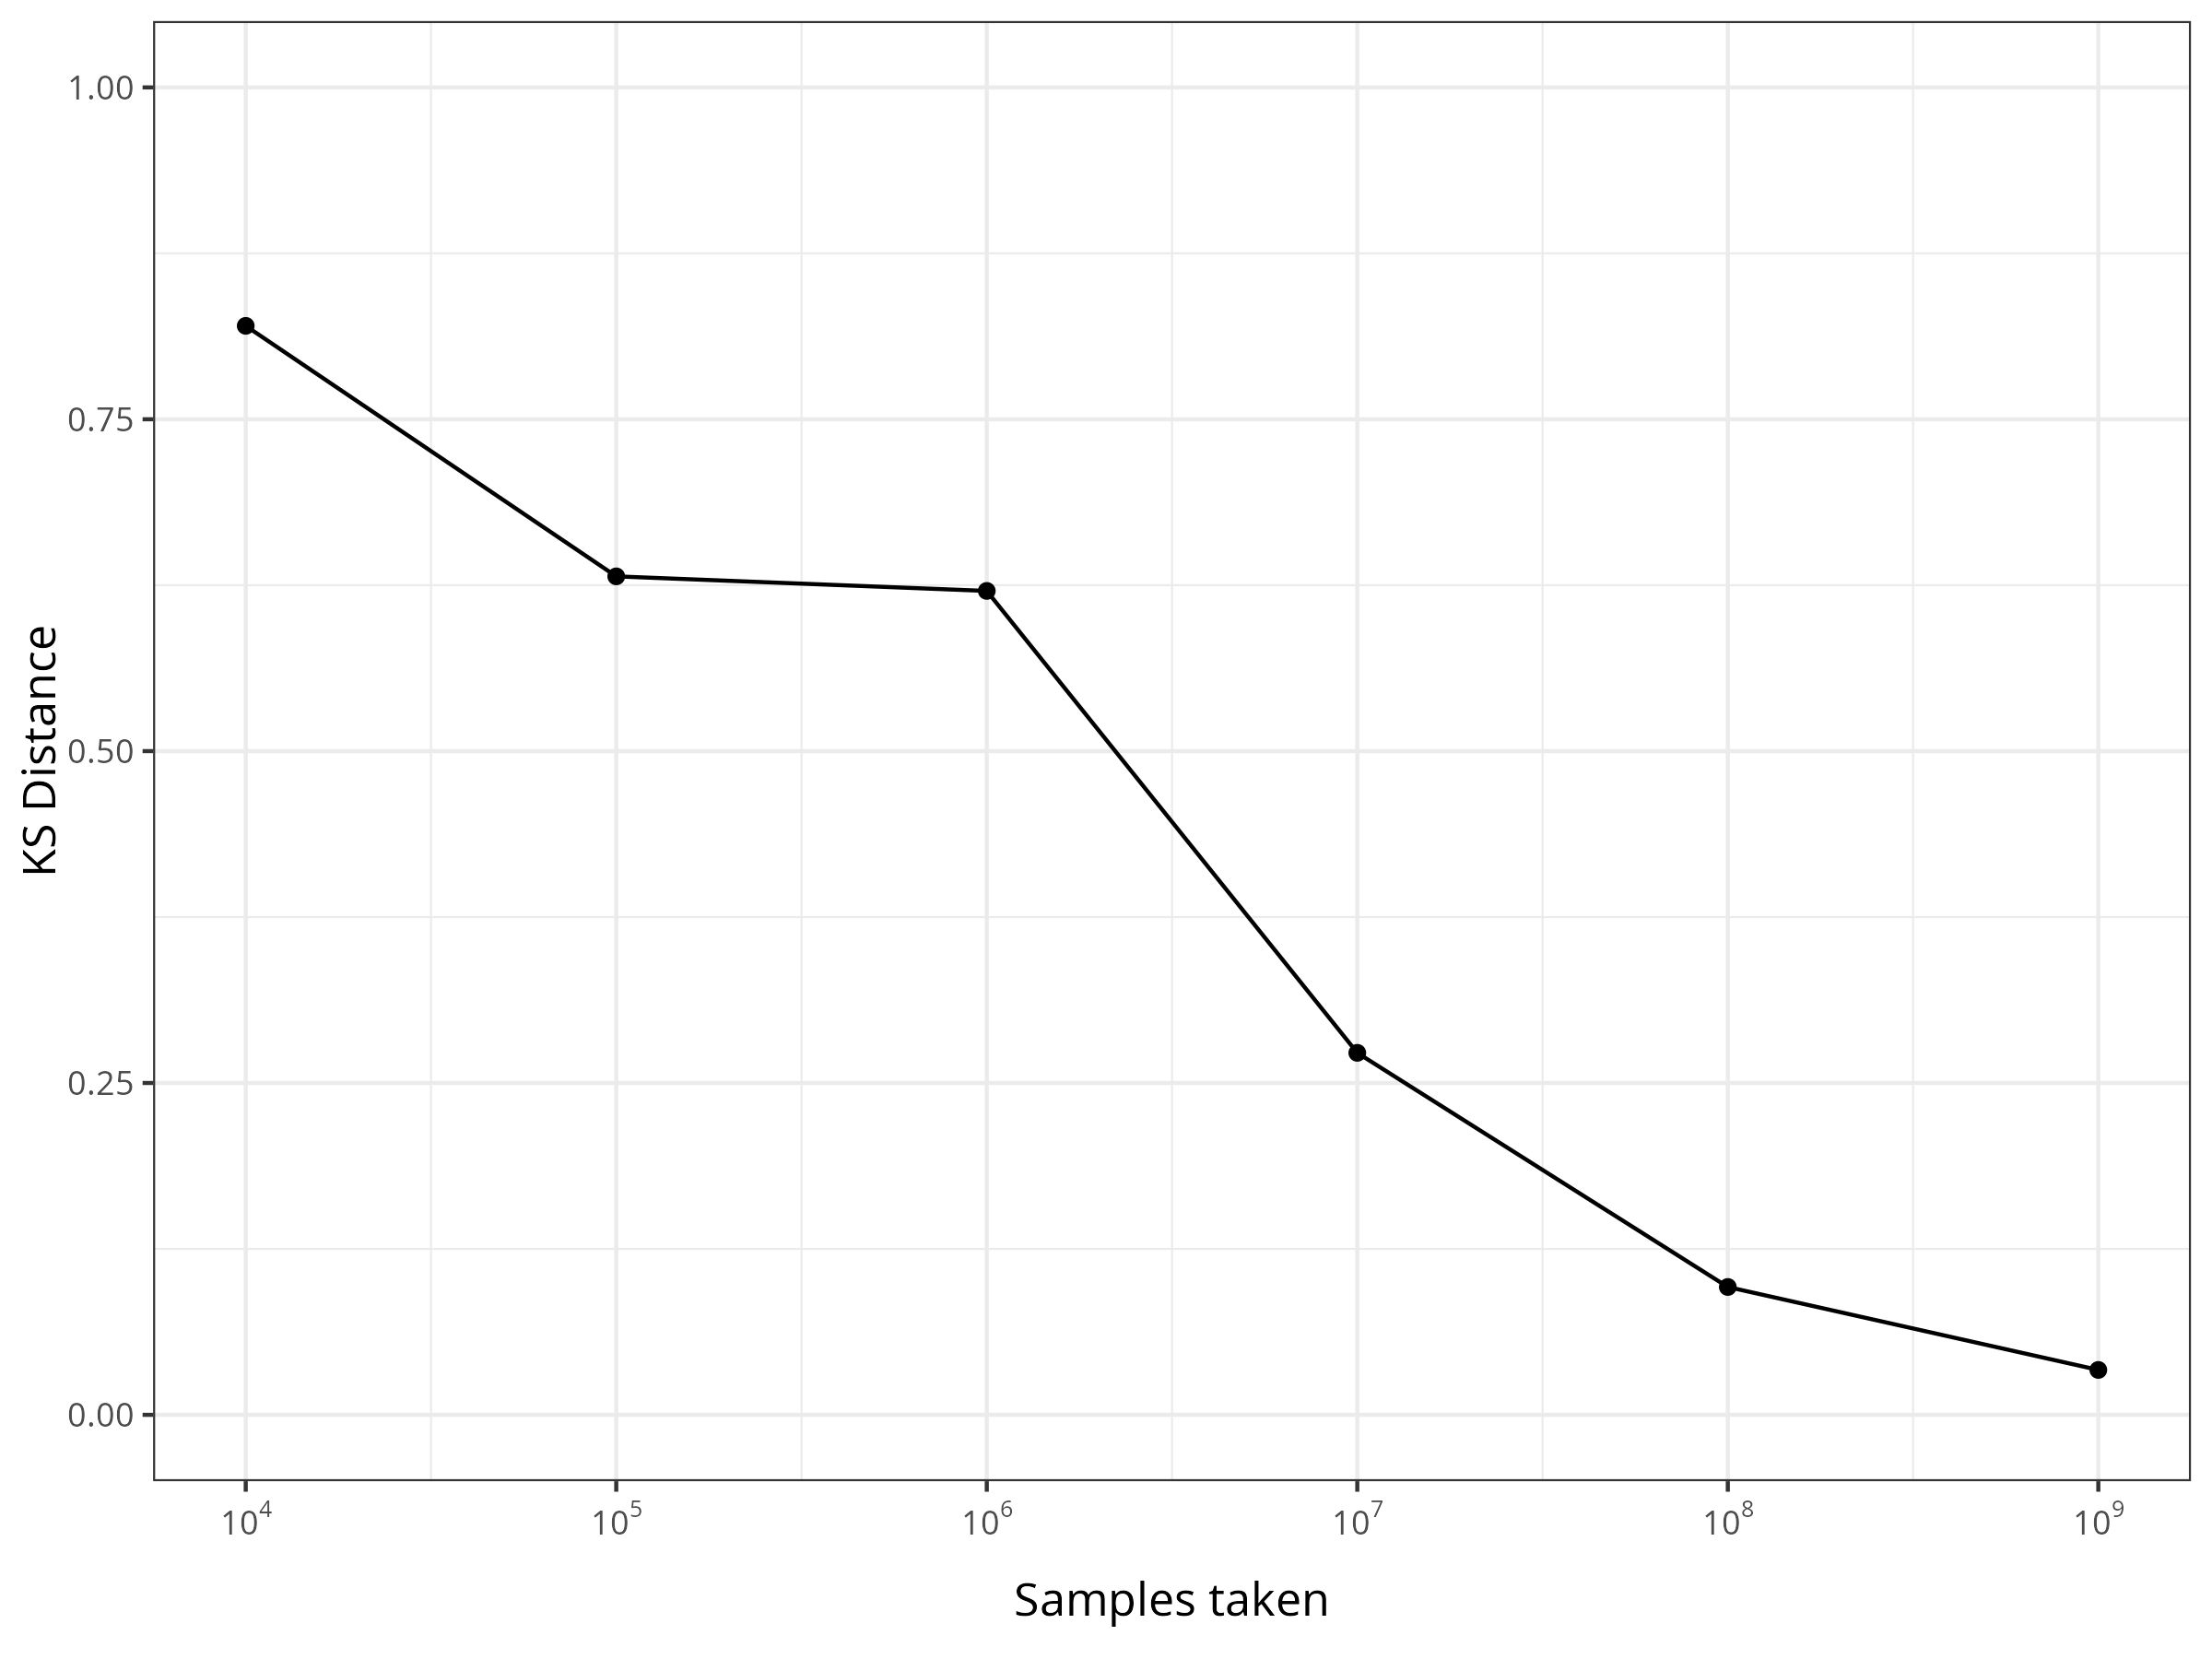
\includegraphics[width=\textwidth]{figures/ks/ycsb.png}
        \caption{YCSB}
    \end{subfigure}
    
    \vspace{1em}

    % Second row
    \begin{subfigure}{0.46\textwidth}
        \centering
        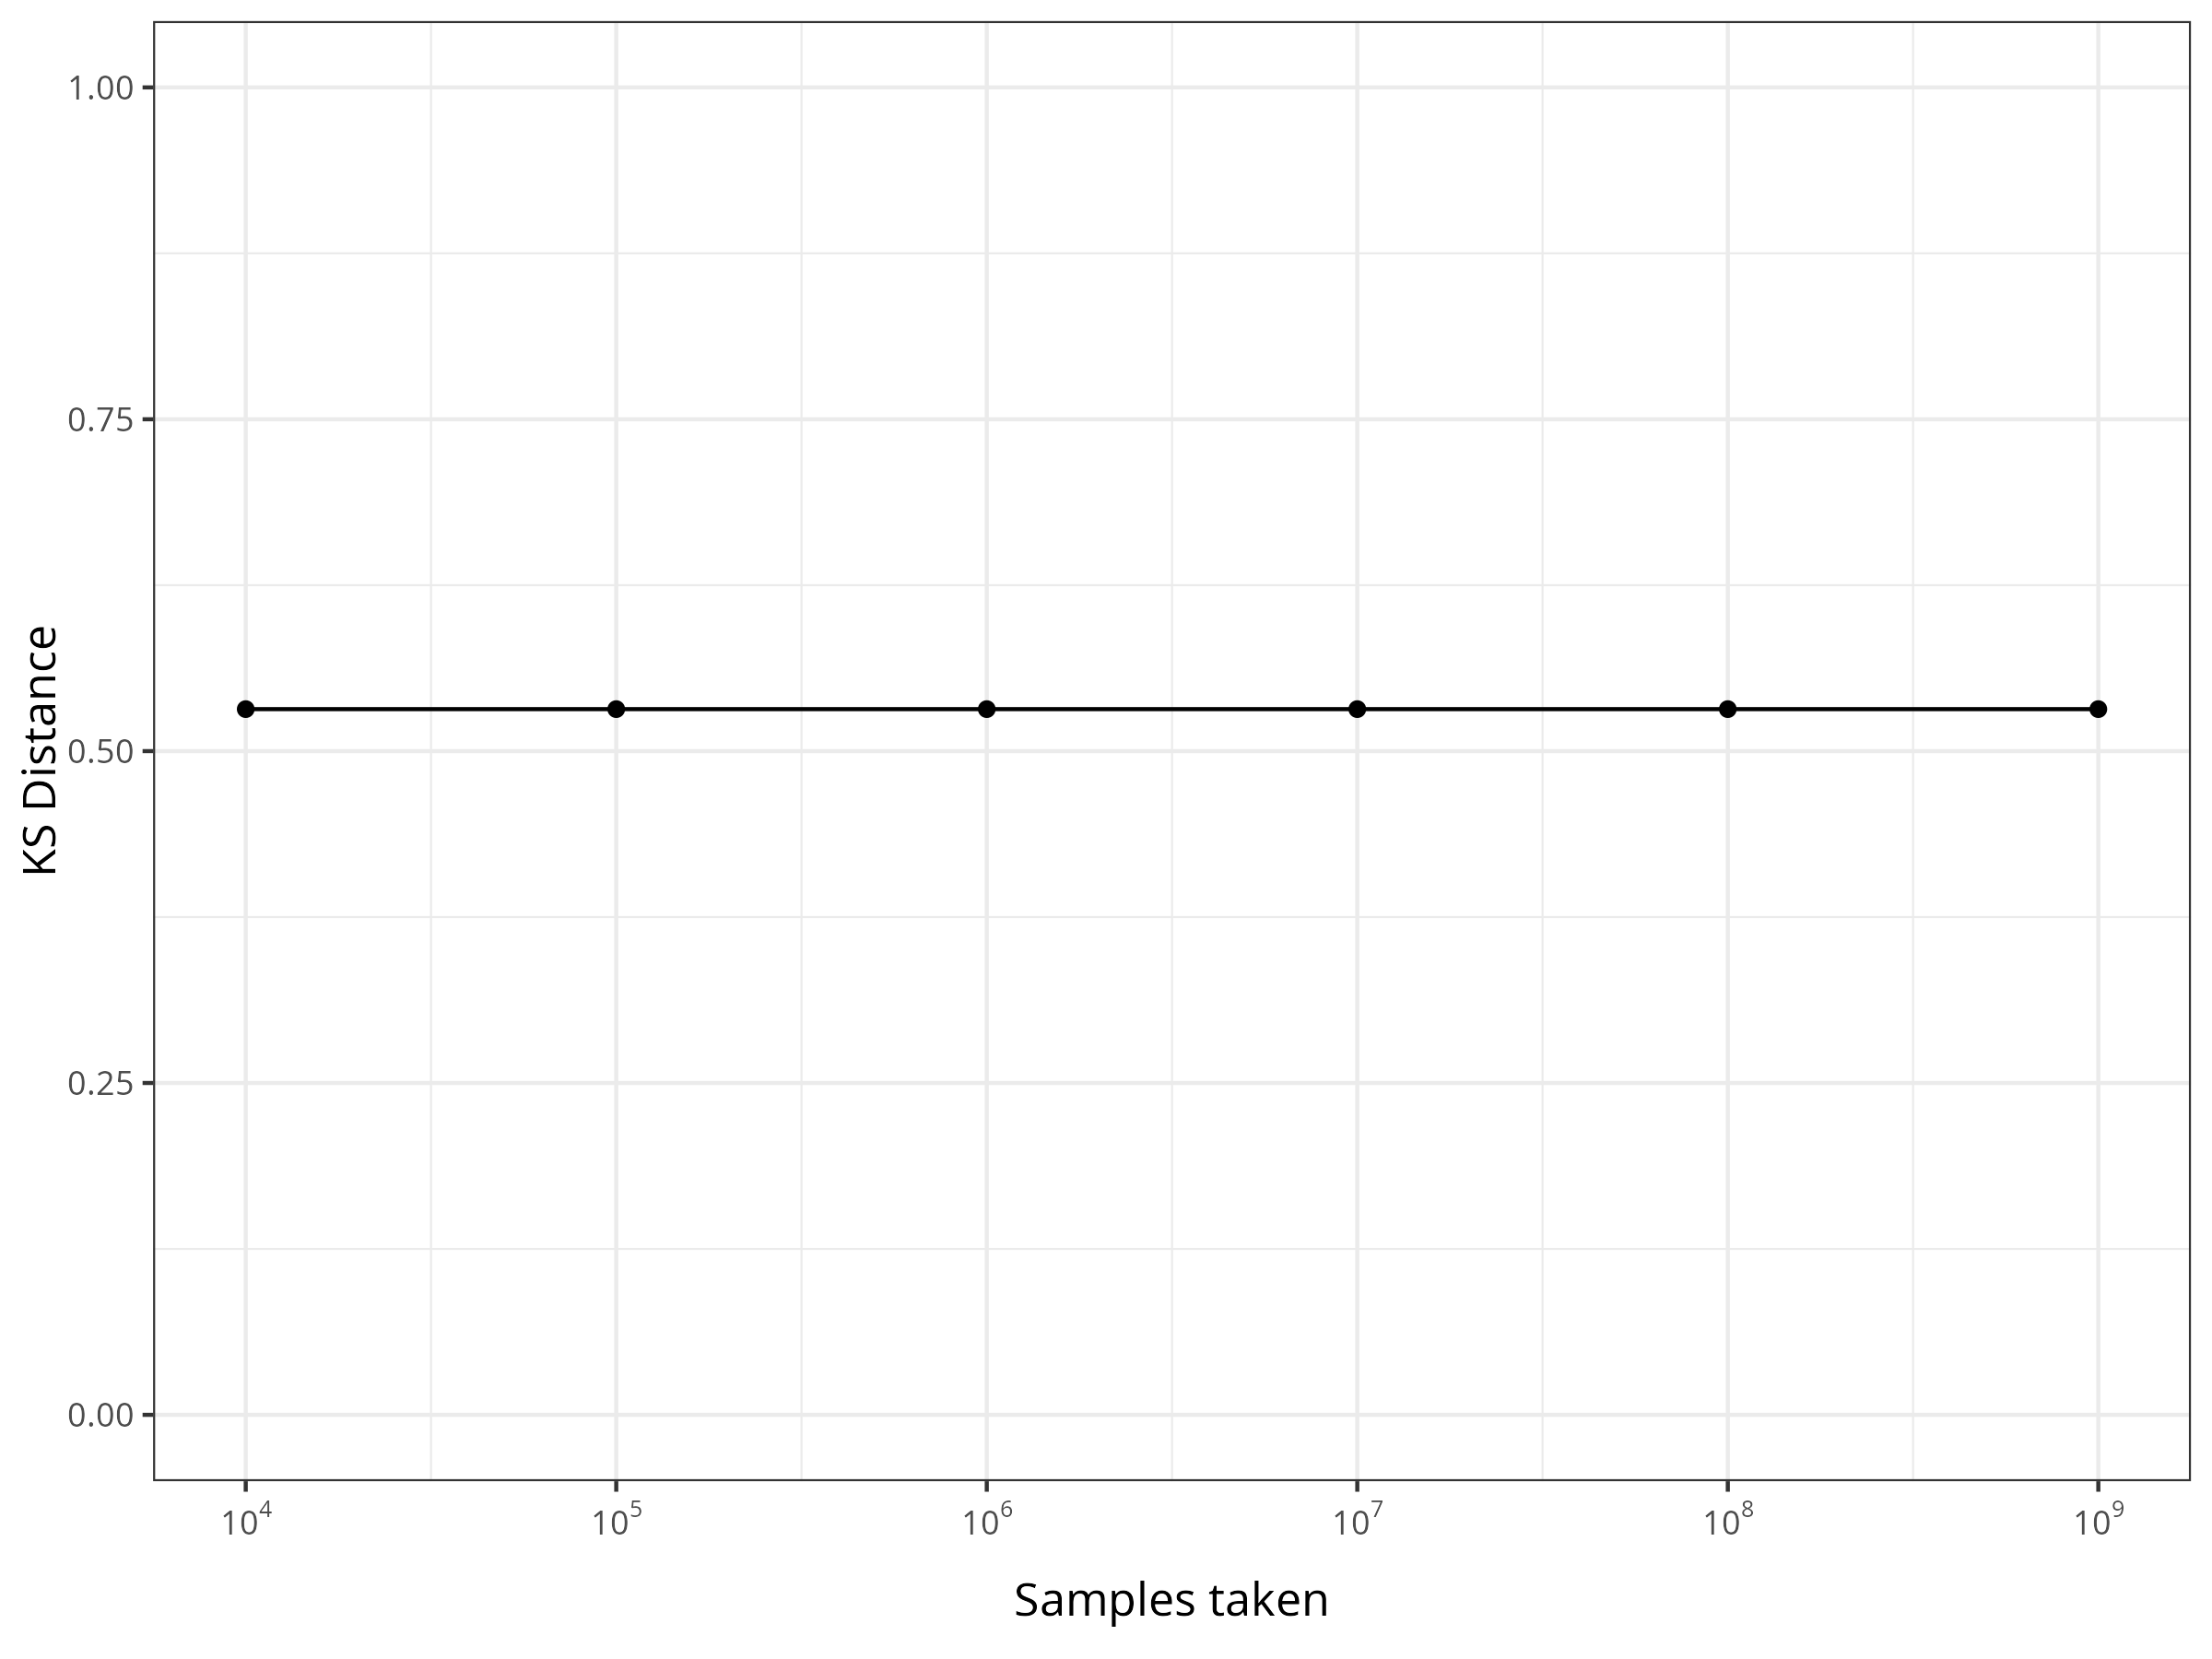
\includegraphics[width=\textwidth]{figures/ks/fio.png}
        \caption{FIO}
    \end{subfigure}
    \hfill
    \begin{subfigure}{0.46\textwidth}
        \centering
        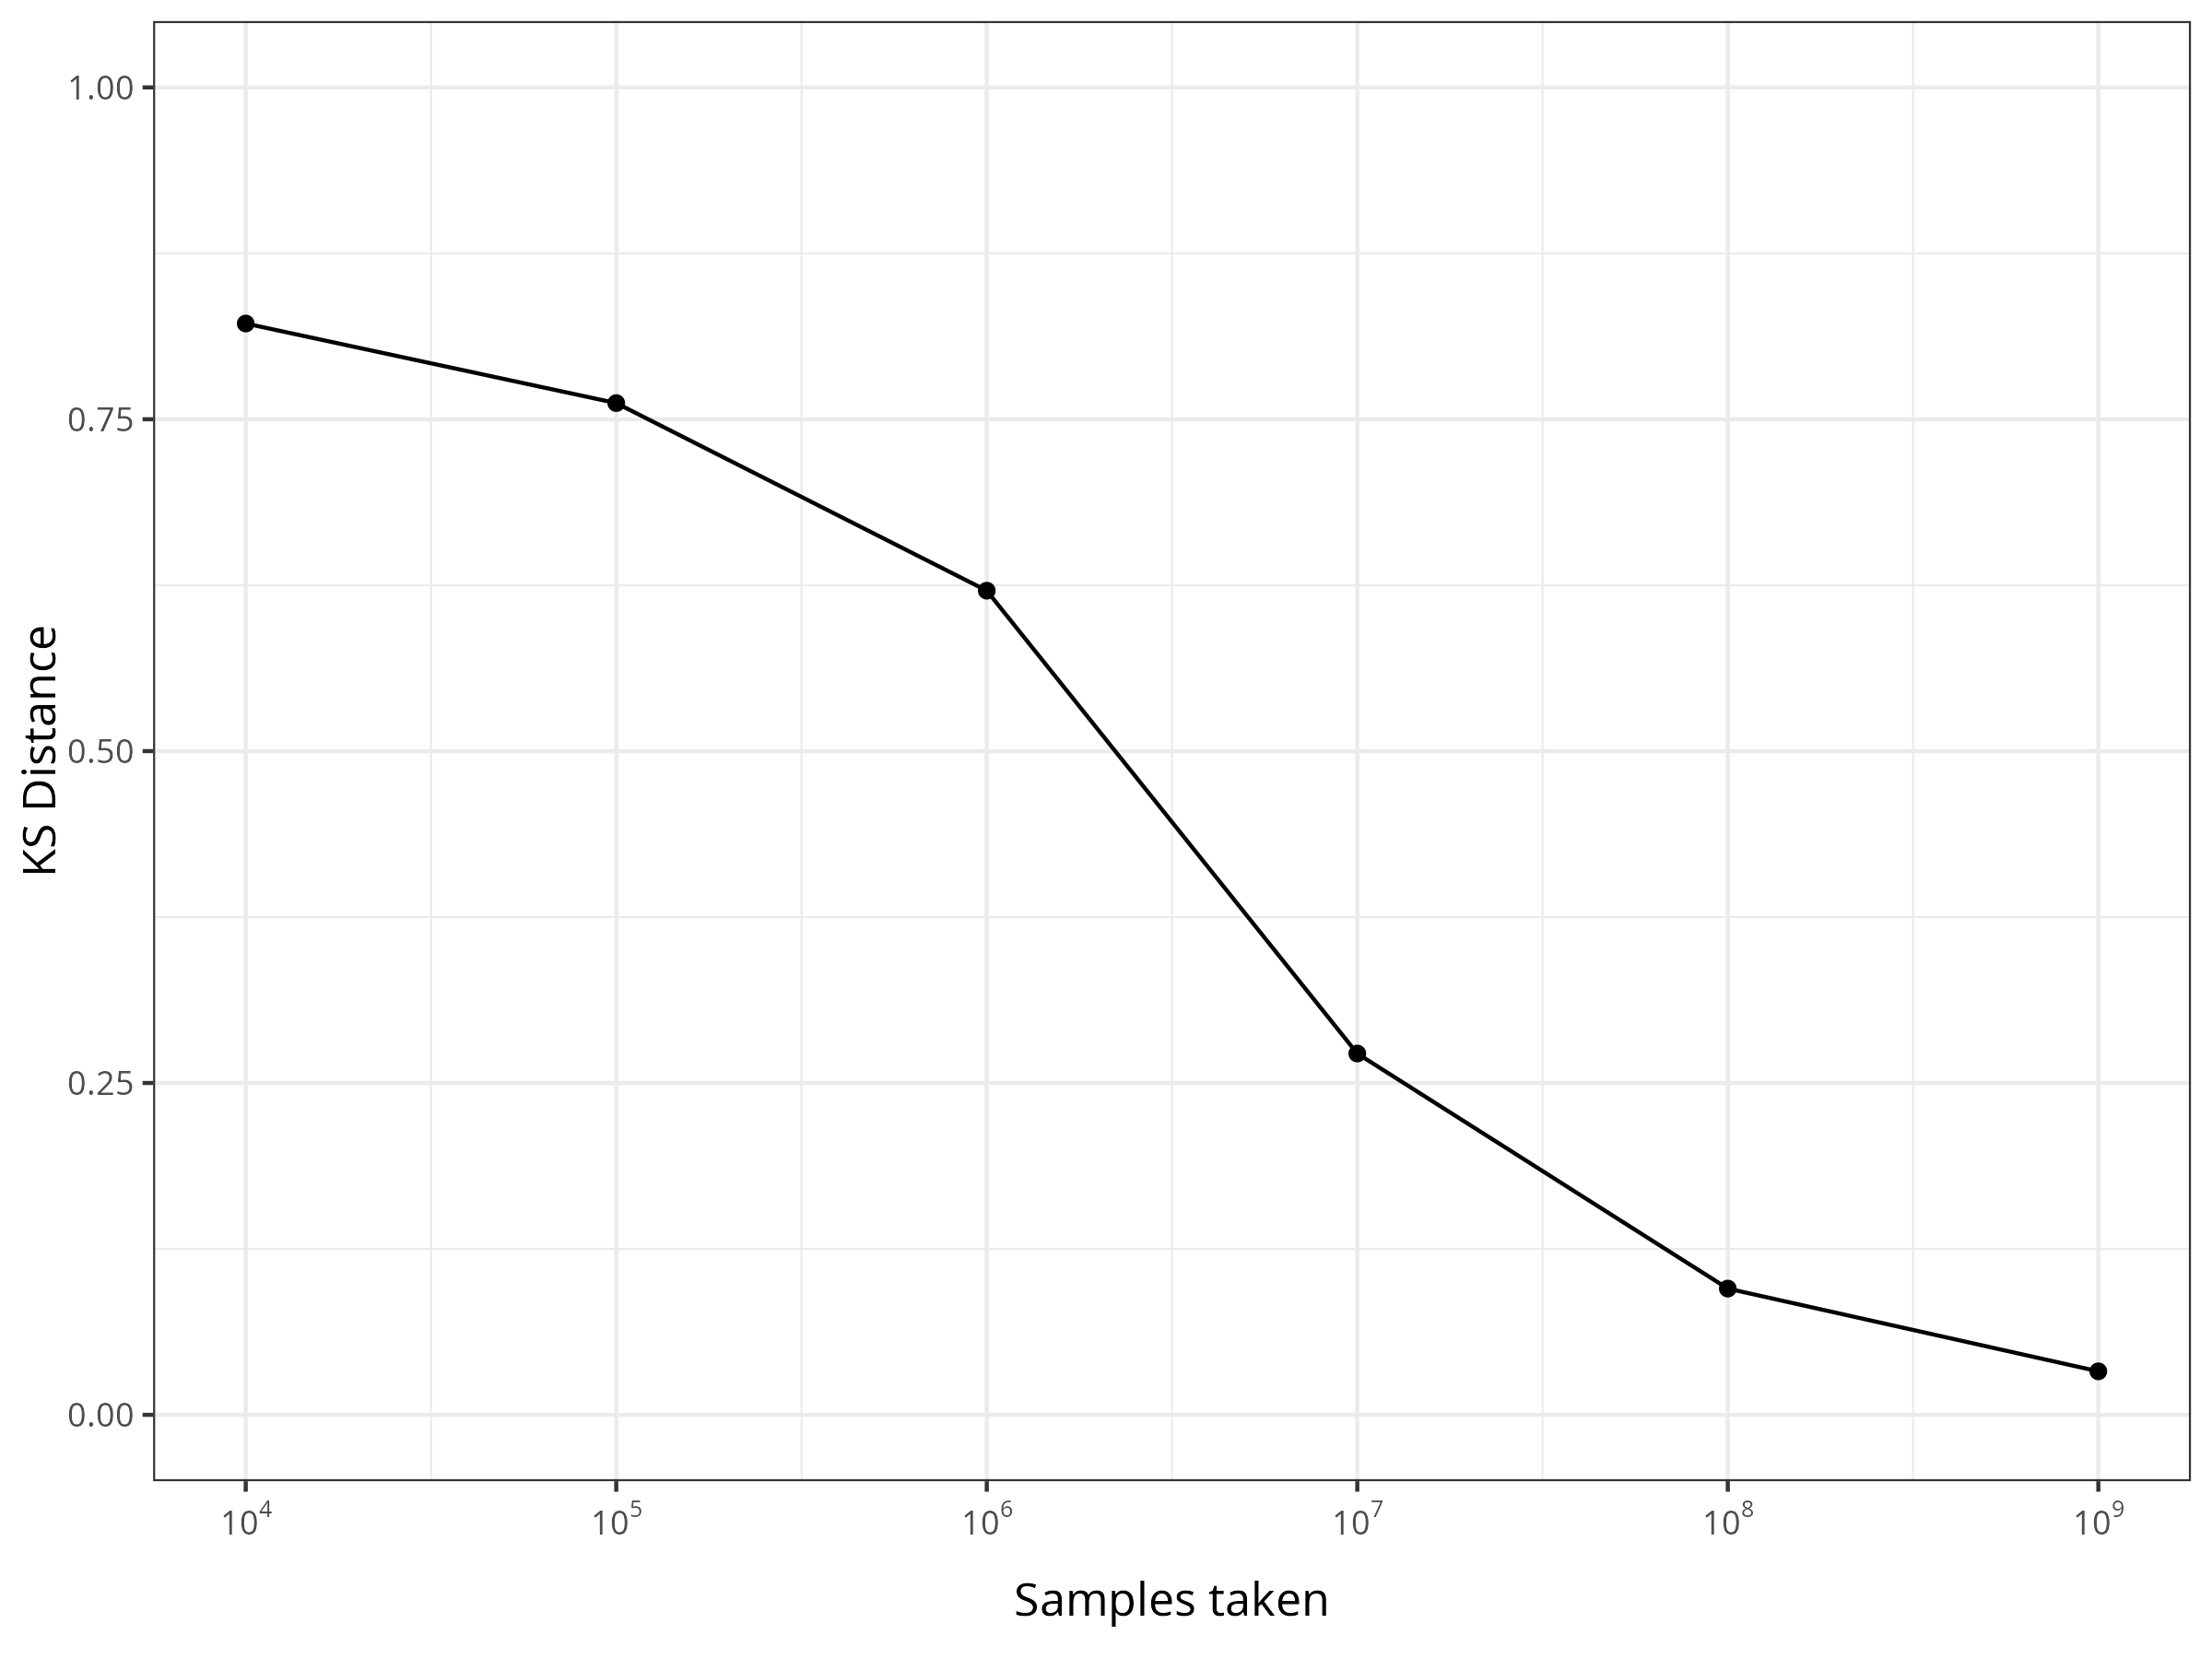
\includegraphics[width=\textwidth]{figures/ks/sysbench.png}
        \caption{Sysbench}
    \end{subfigure}
    
    \vspace{1em}

    % Third row
    \begin{subfigure}{0.46\textwidth}
        \centering
        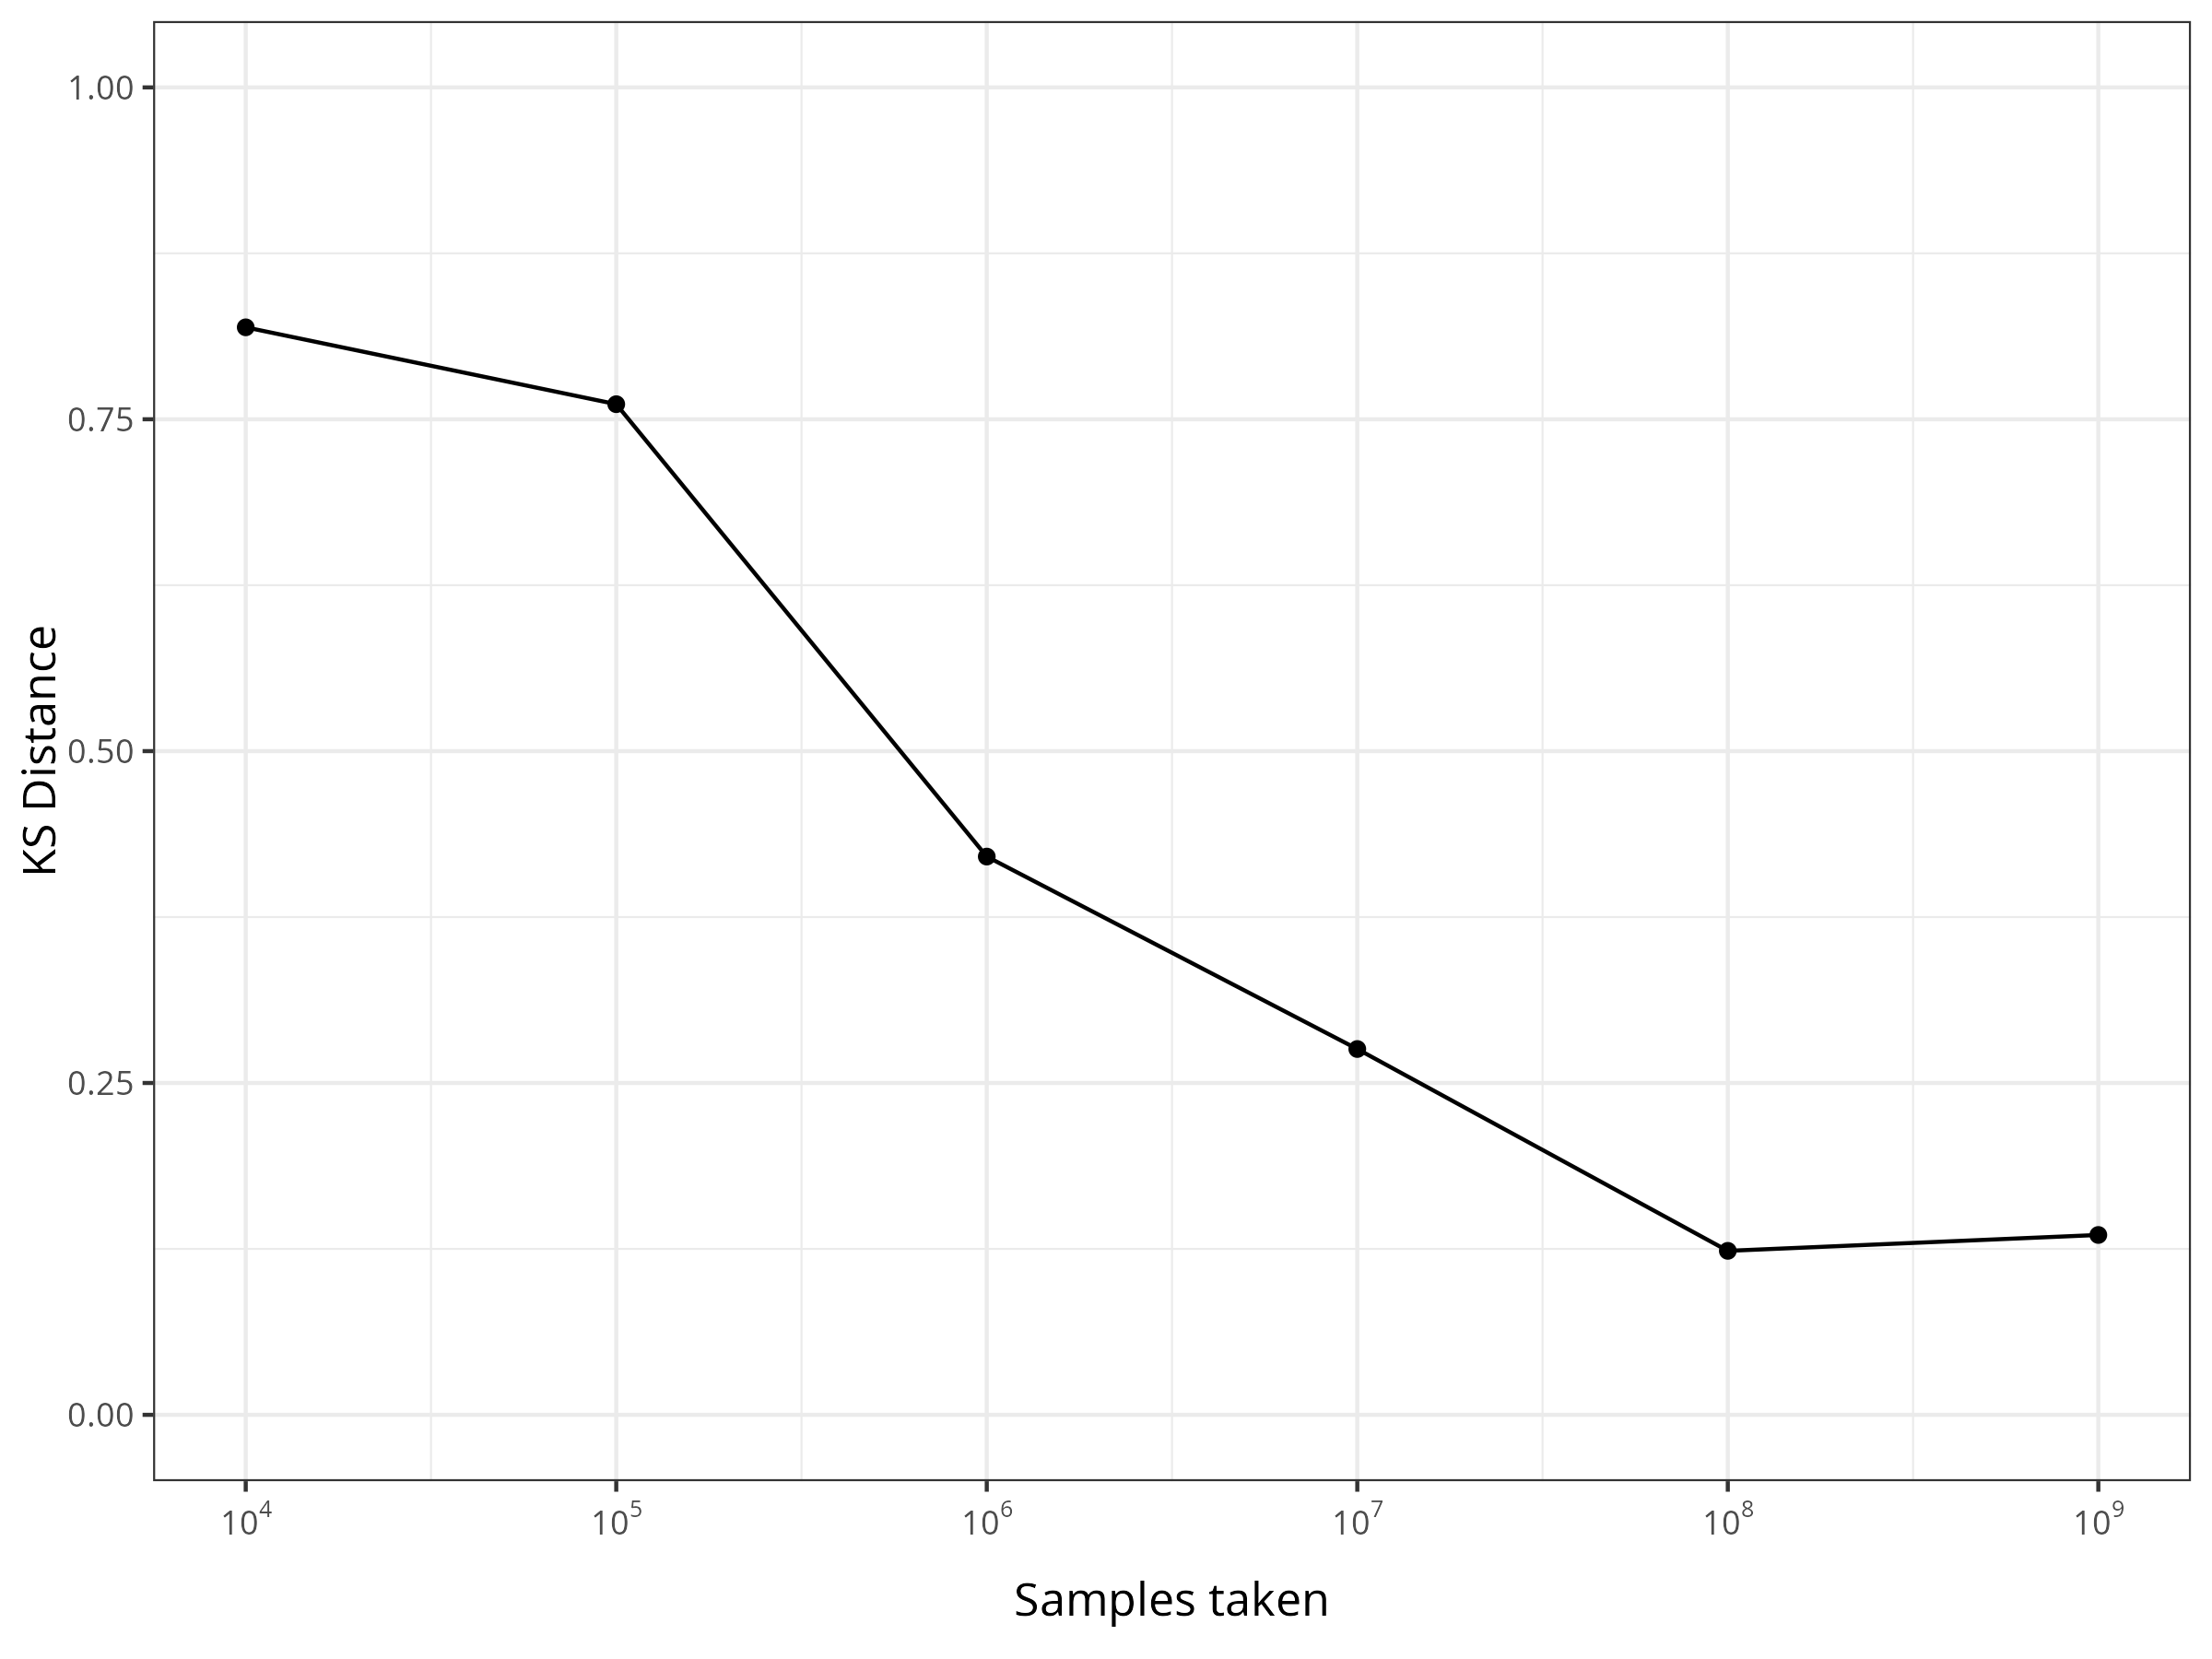
\includegraphics[width=\textwidth]{figures/ks/marsaglia.png}
        \caption{Condensed Table Lookup}
    \end{subfigure}
    \hfill
    \begin{subfigure}{0.46\textwidth}
        \centering
        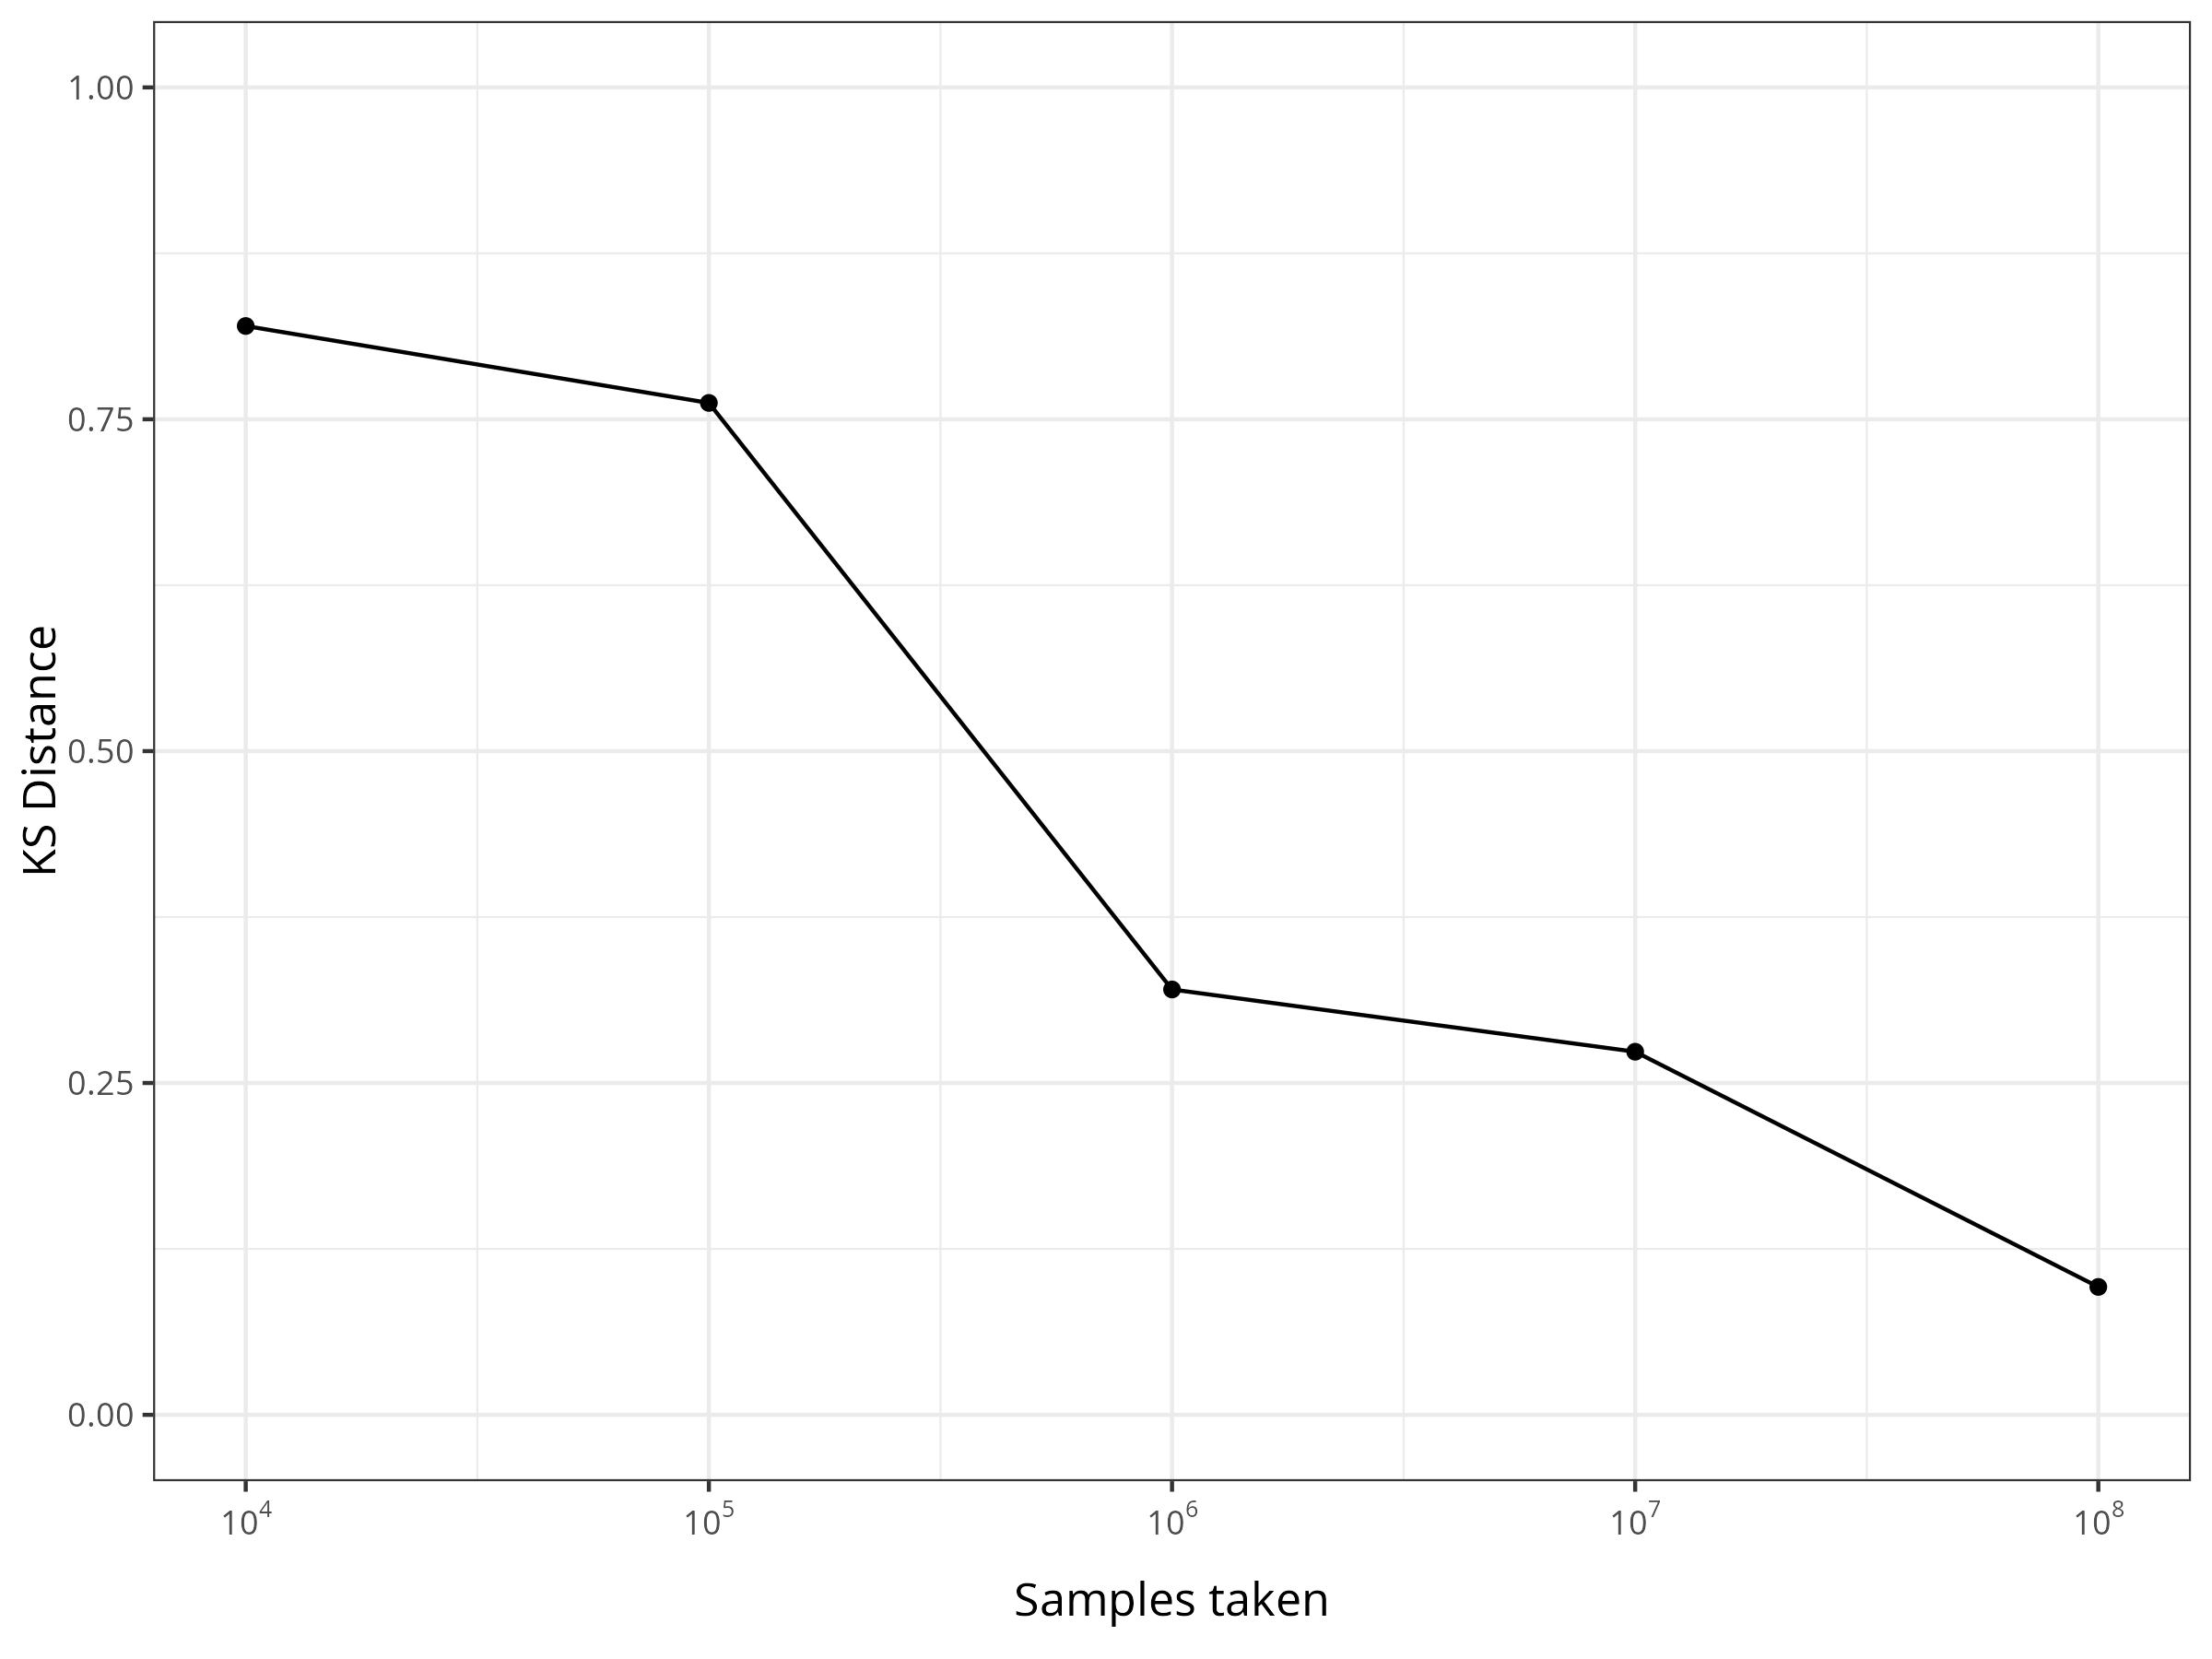
\includegraphics[width=\textwidth]{figures/ks/rejection.png}
        \caption{Rejection Sampling}
    \end{subfigure}

    \caption{Kolmogorov-Smirnov test results for the different samplers.}
    \label{fig:ks_graphs}
\end{figure}

\begin{figure}[t]
    % First row
    \centering
    \begin{subfigure}{0.46\textwidth}
        \centering
        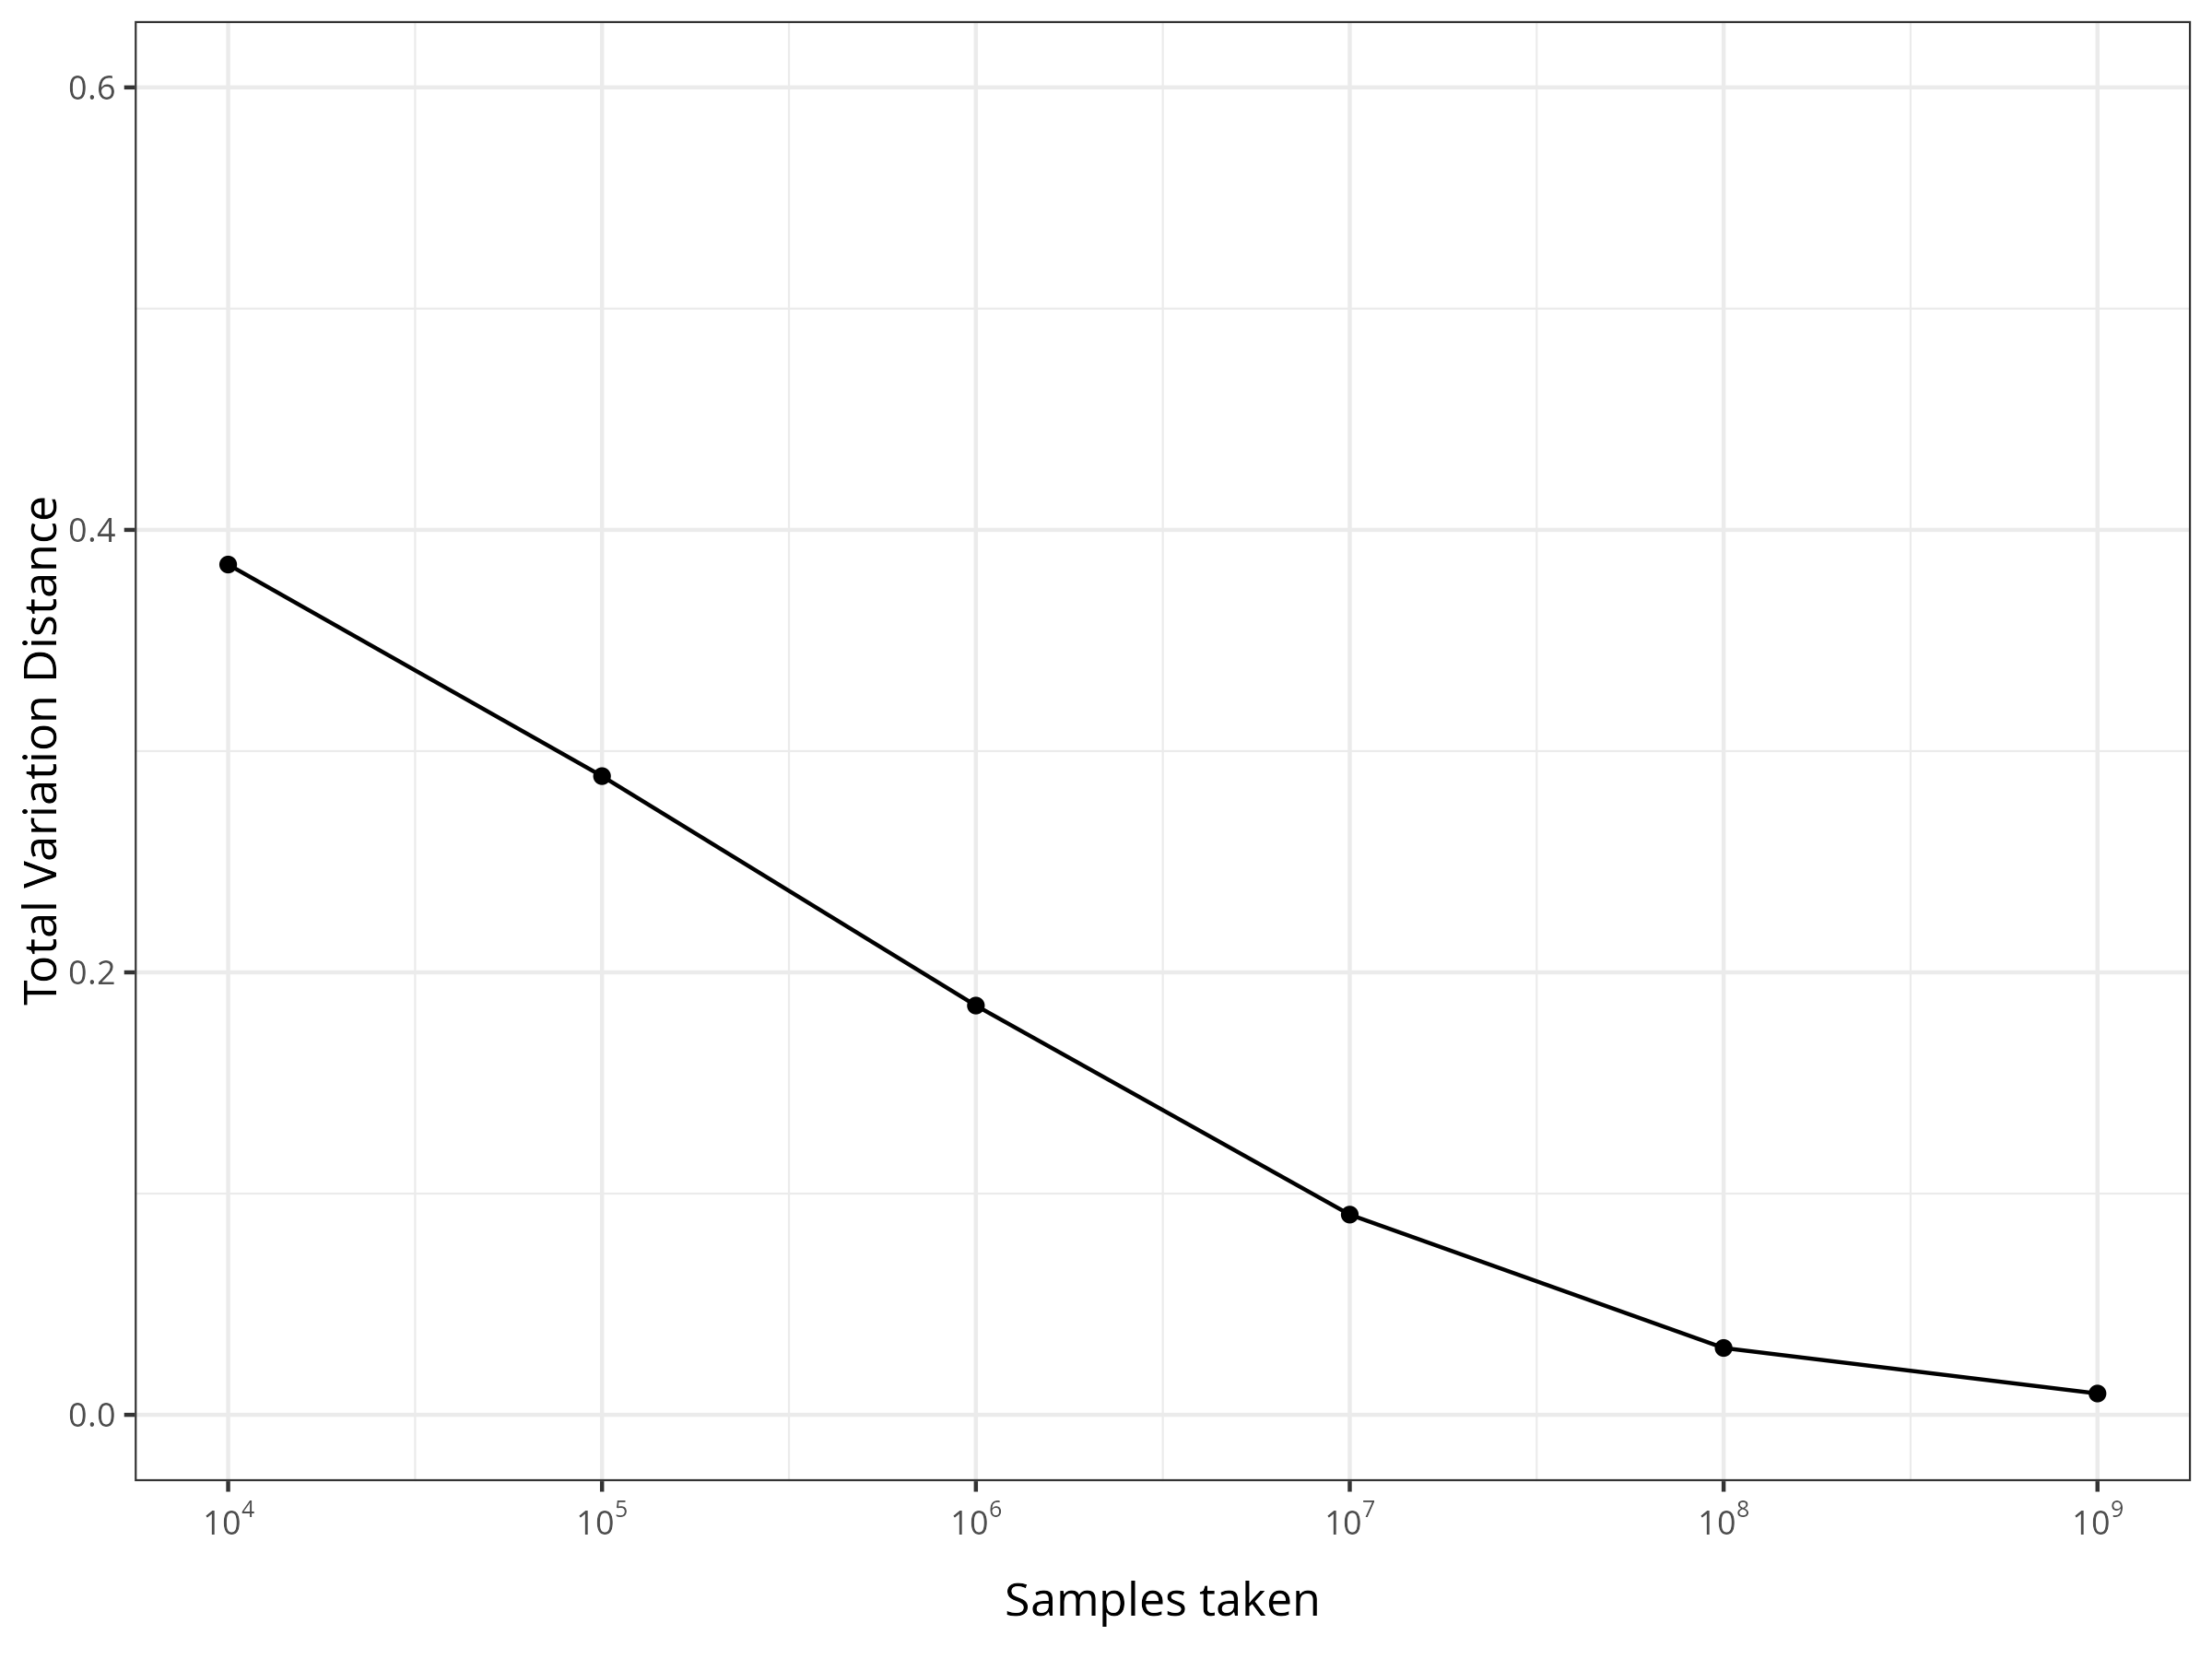
\includegraphics[width=\textwidth]{figures/tvd/apache.png}
        \caption{Rejection-Inversion}
    \end{subfigure}
    \hfill
    \begin{subfigure}{0.46\textwidth}
        \centering
        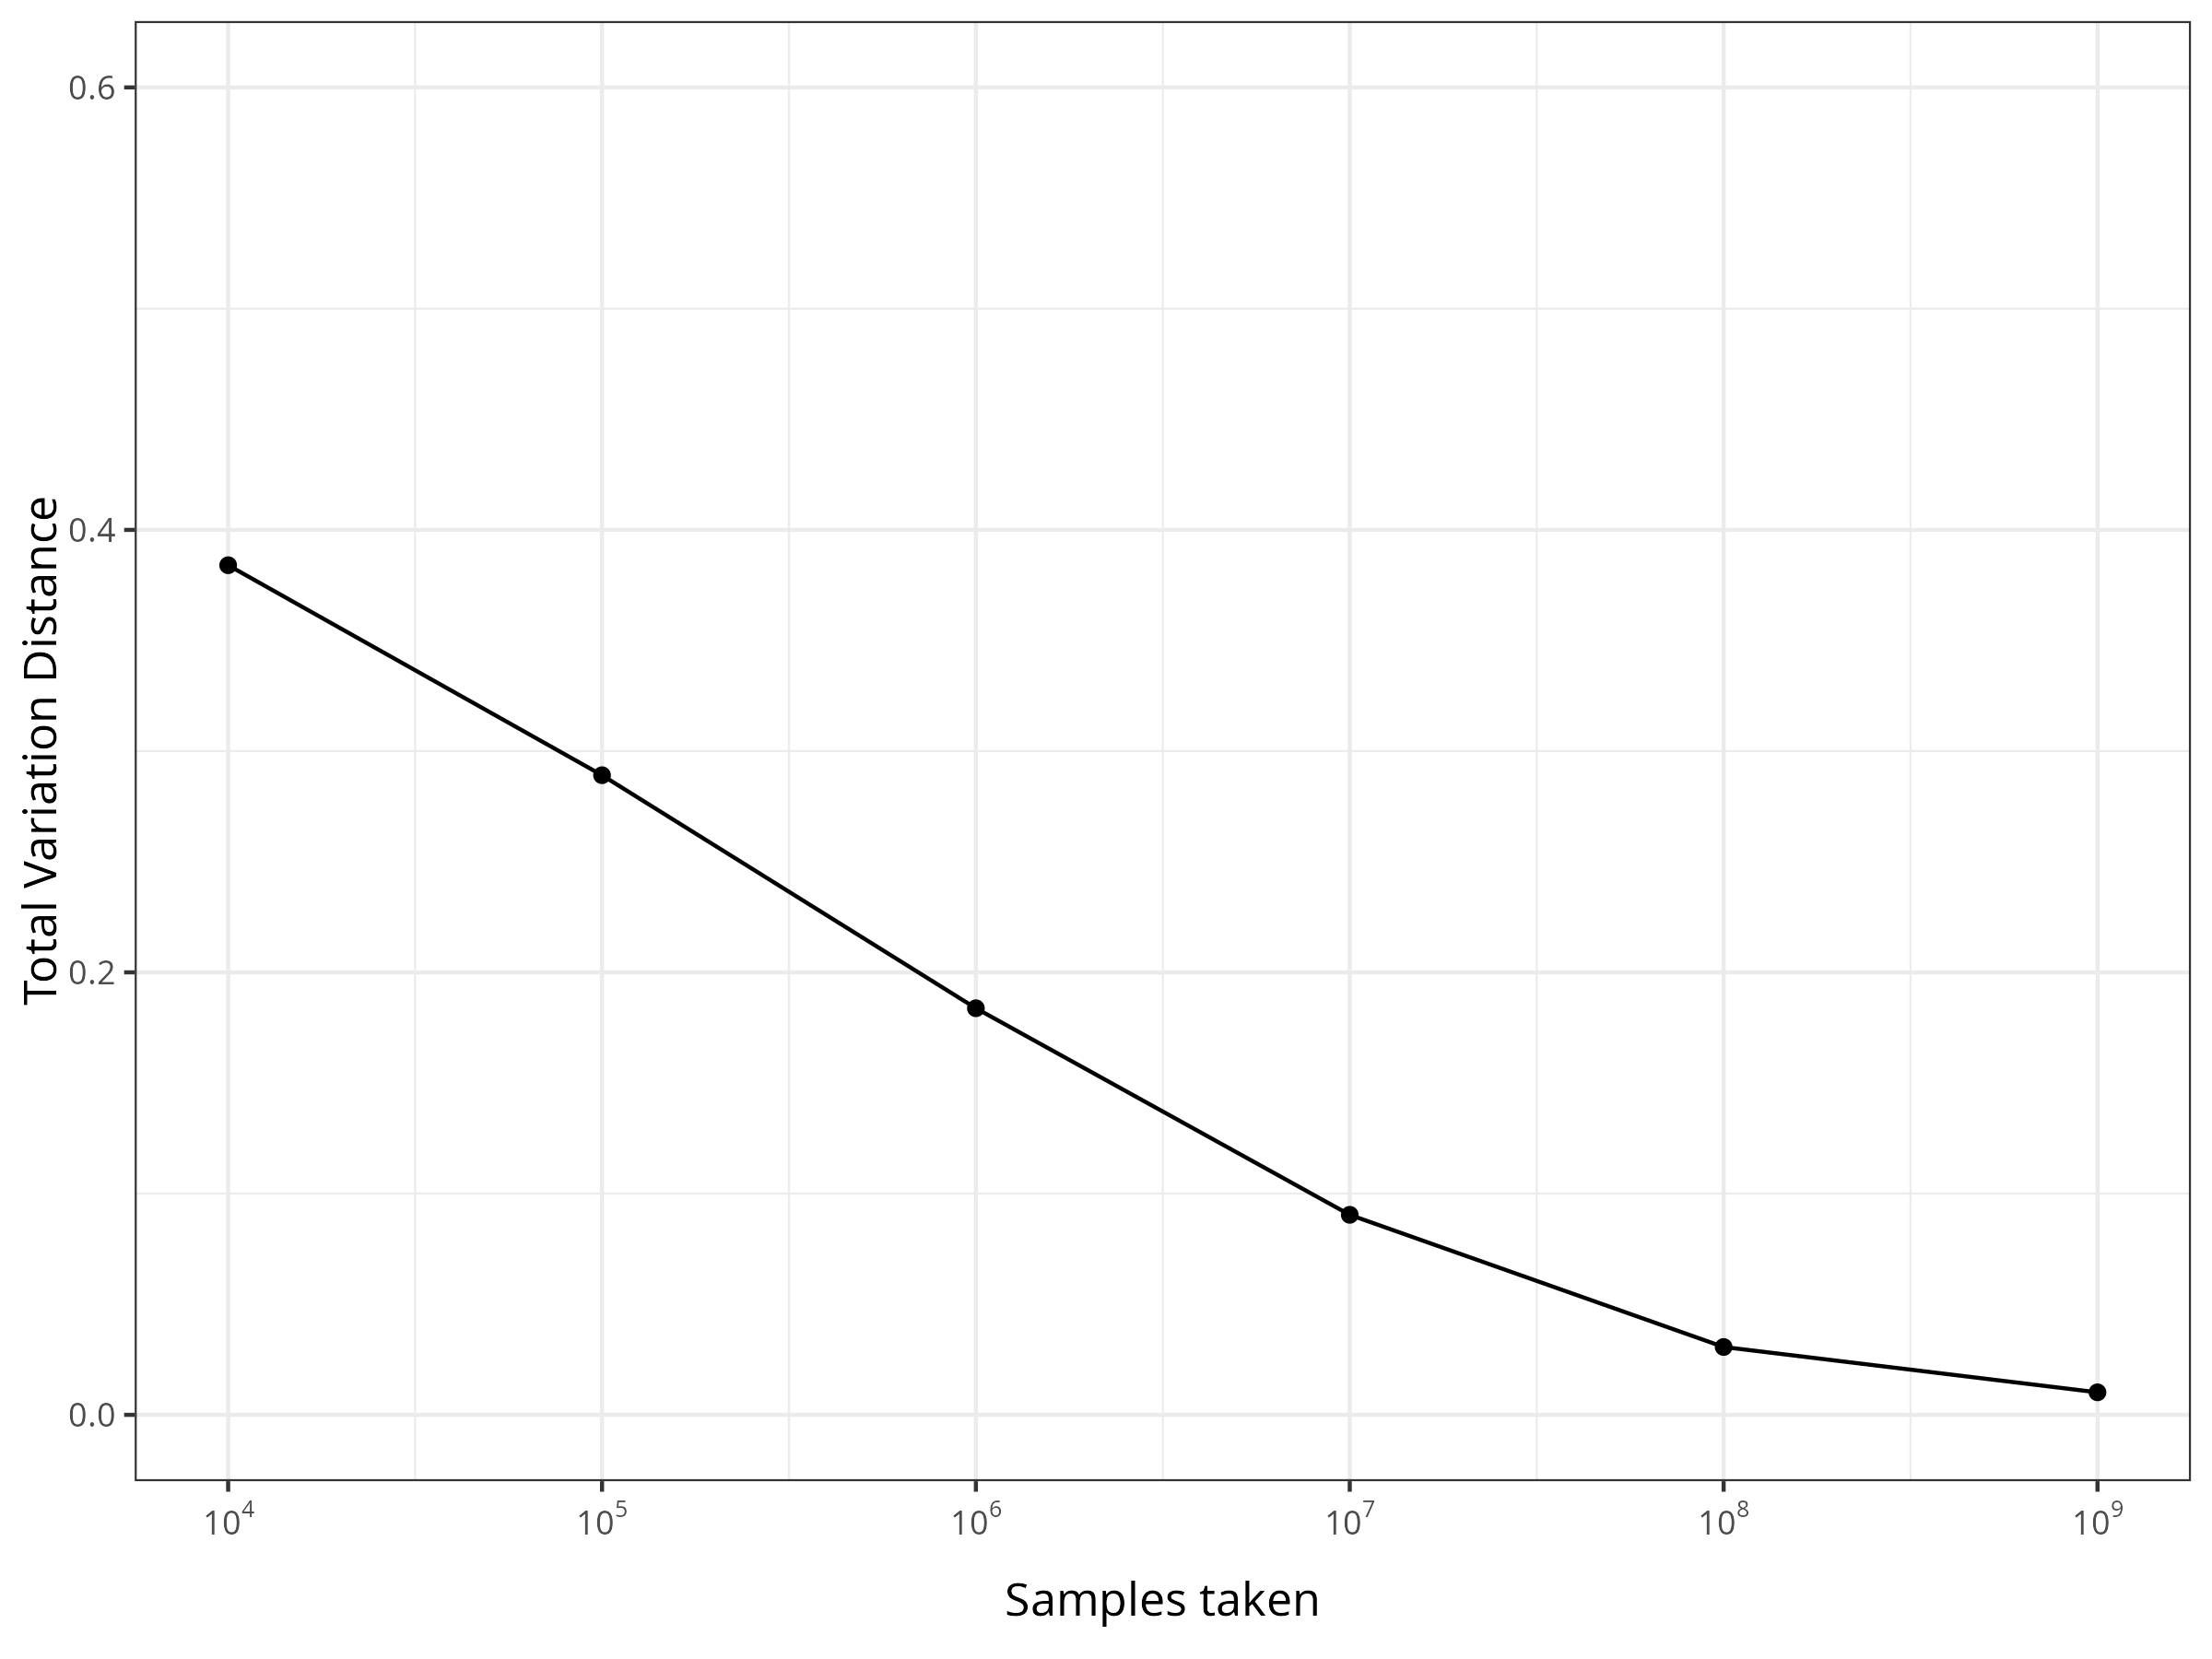
\includegraphics[width=\textwidth]{figures/tvd/ycsb.png}
        \caption{YCSB}
    \end{subfigure}
    
    \vspace{1em}

    % Second row
    \begin{subfigure}{0.46\textwidth}
        \centering
        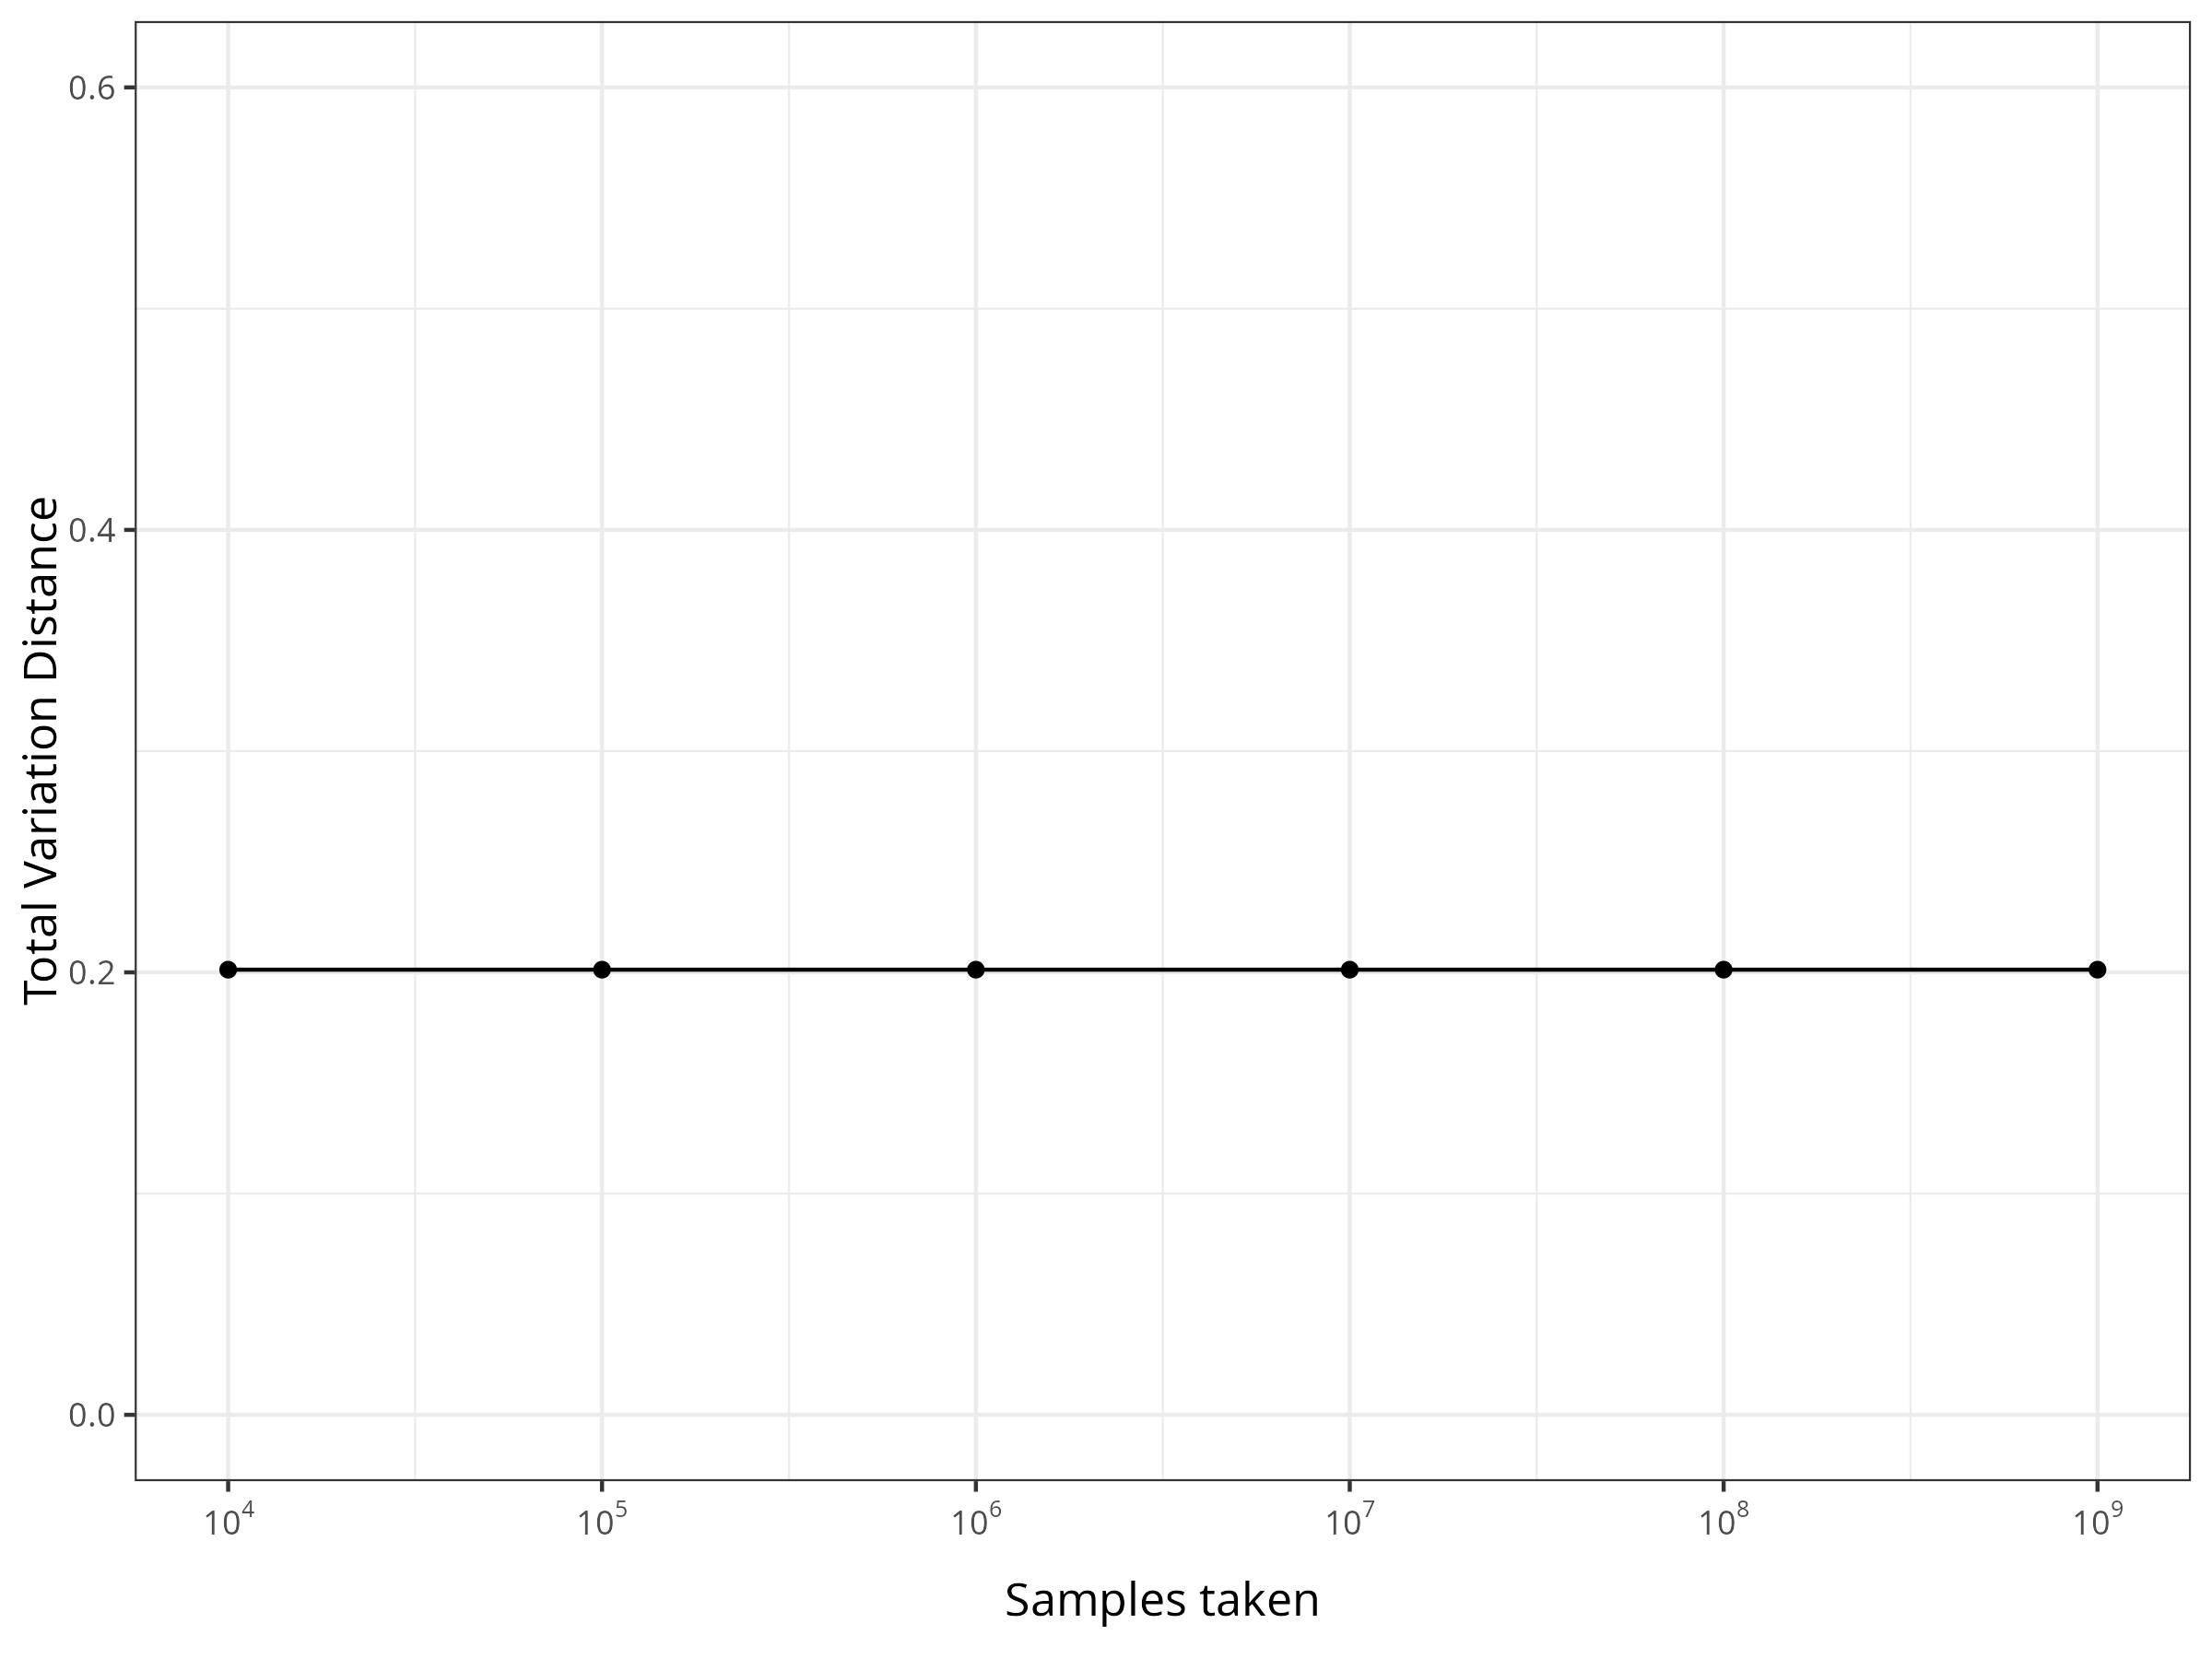
\includegraphics[width=\textwidth]{figures/tvd/fio.png}
        \caption{FIO}
    \end{subfigure}
    \hfill
    \begin{subfigure}{0.46\textwidth}
        \centering
        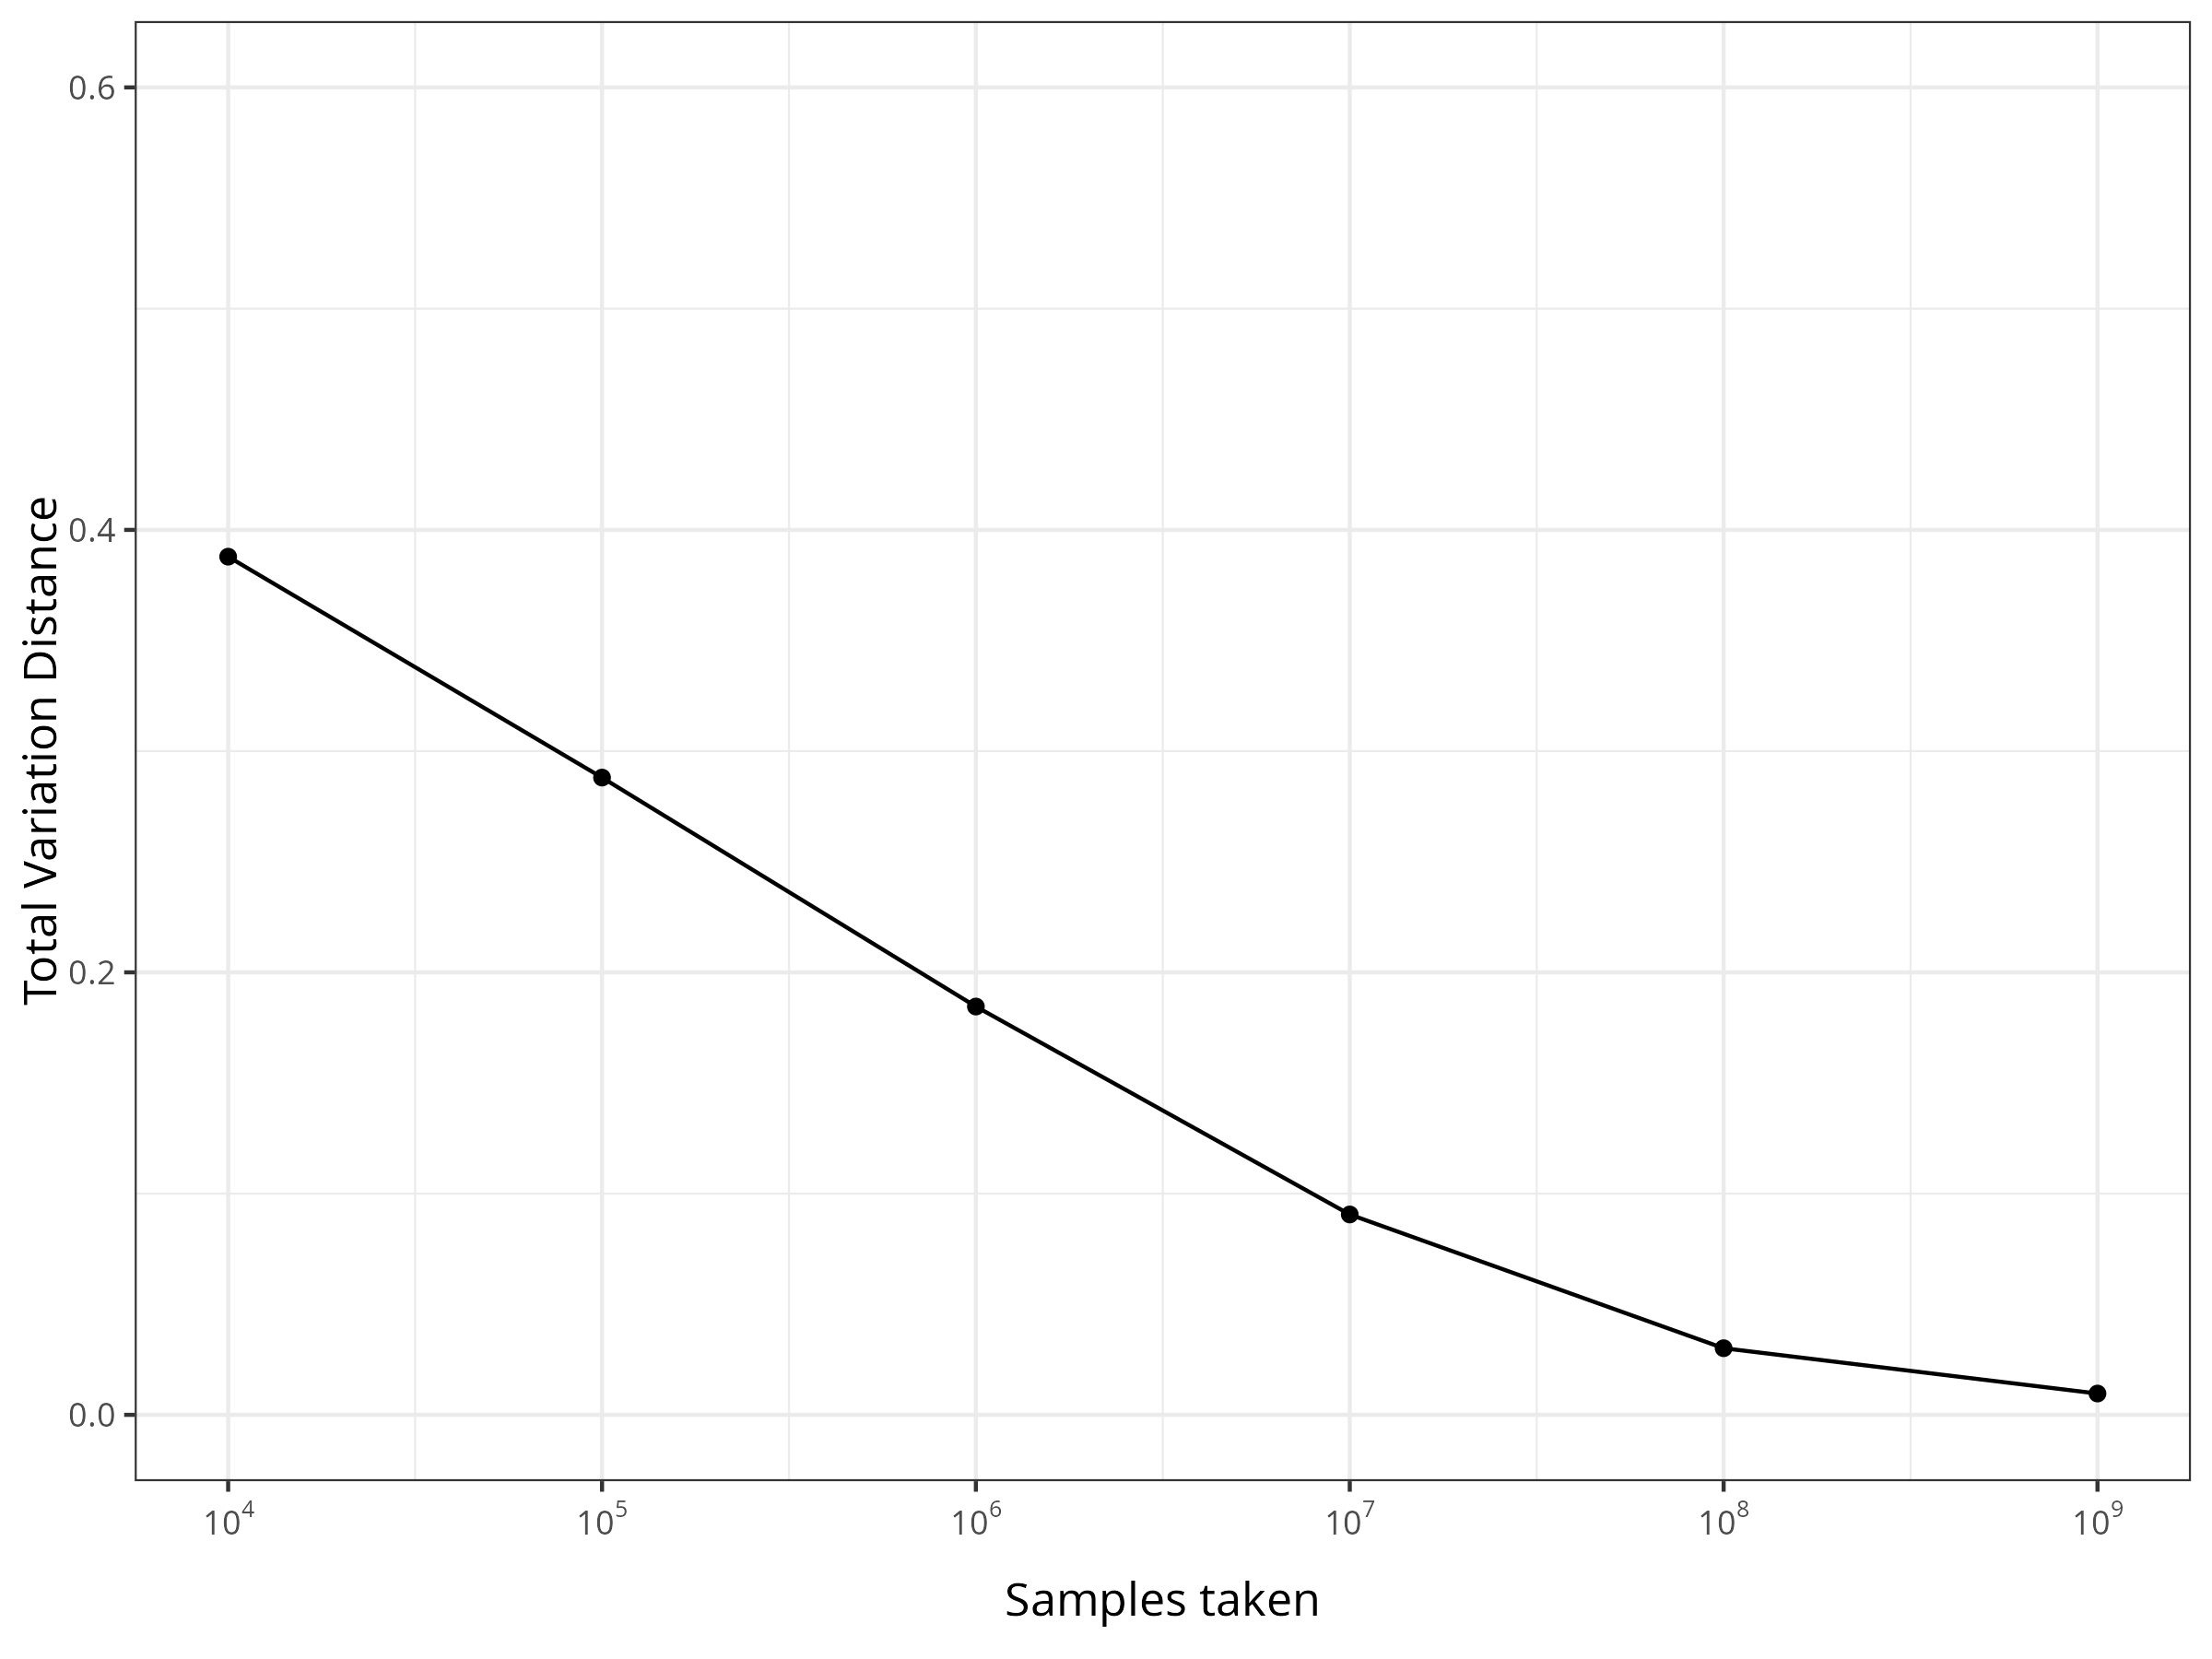
\includegraphics[width=\textwidth]{figures/tvd/sysbench.png}
        \caption{Sysbench}
    \end{subfigure}
    
    \vspace{1em}

    % Third row
    \begin{subfigure}{0.46\textwidth}
        \centering
        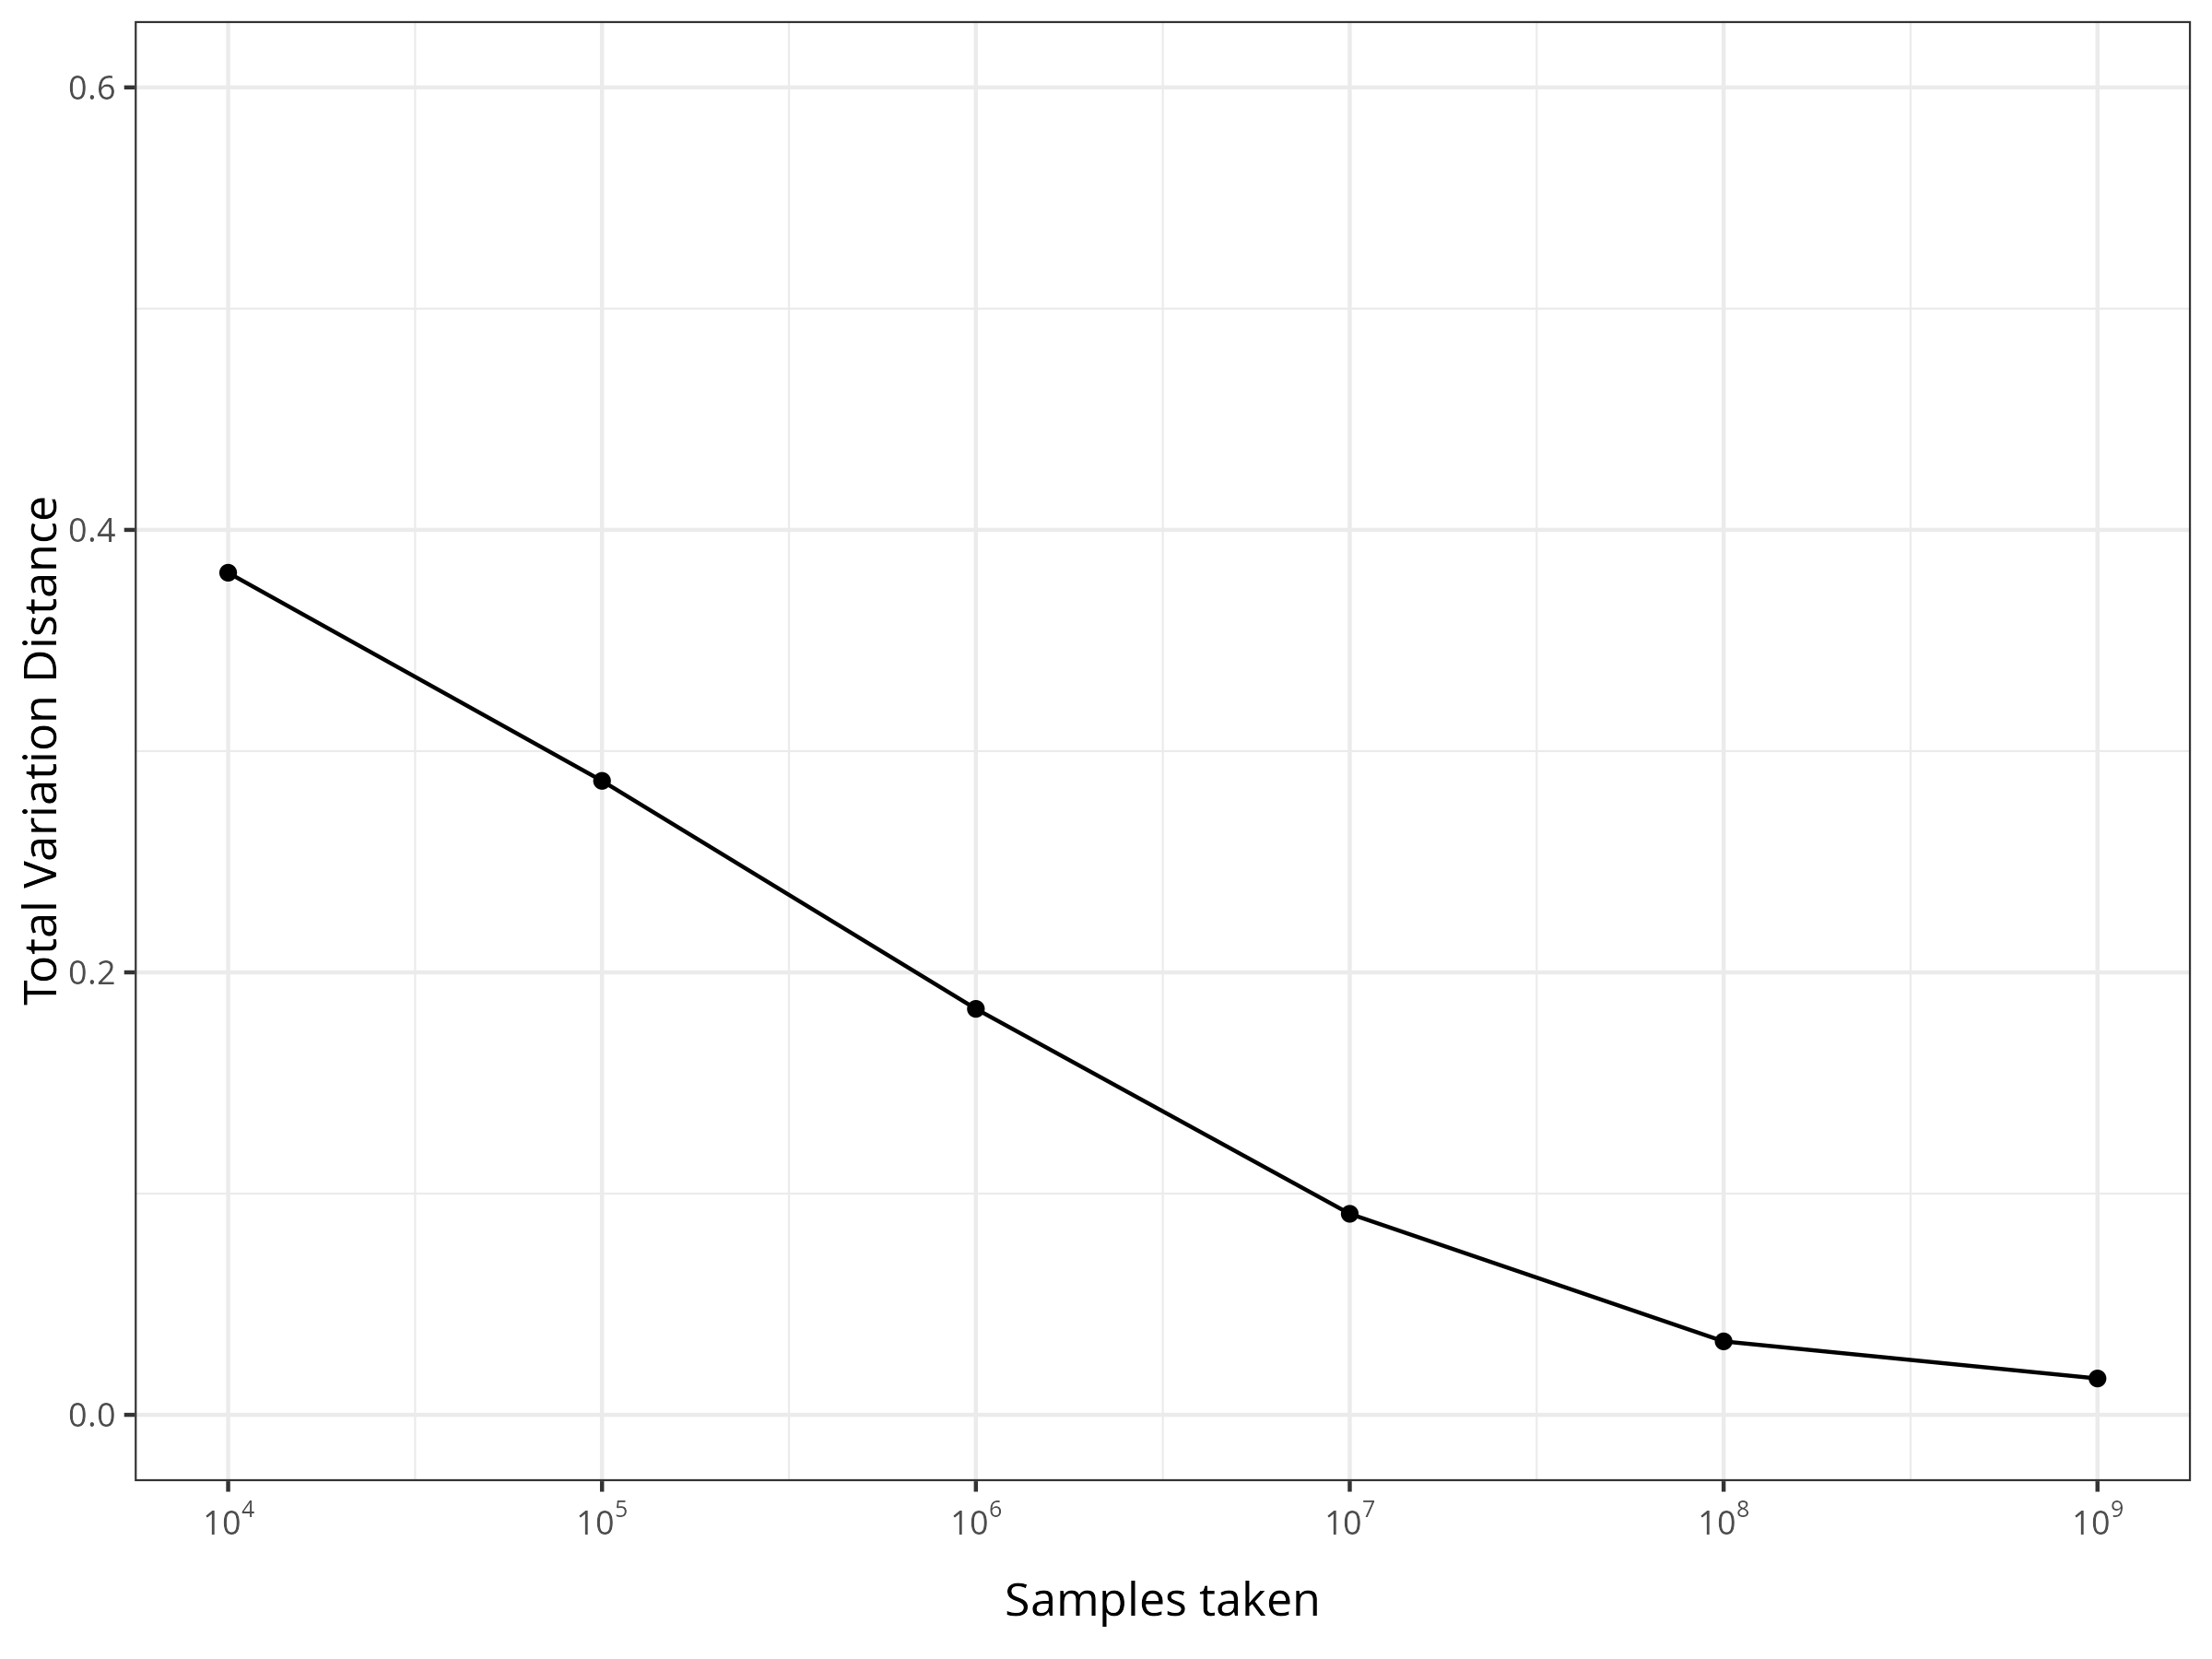
\includegraphics[width=\textwidth]{figures/tvd/marsaglia.png}
        \caption{Condensed Table Lookup}
    \end{subfigure}
    \hfill
    \begin{subfigure}{0.46\textwidth}
        \centering
        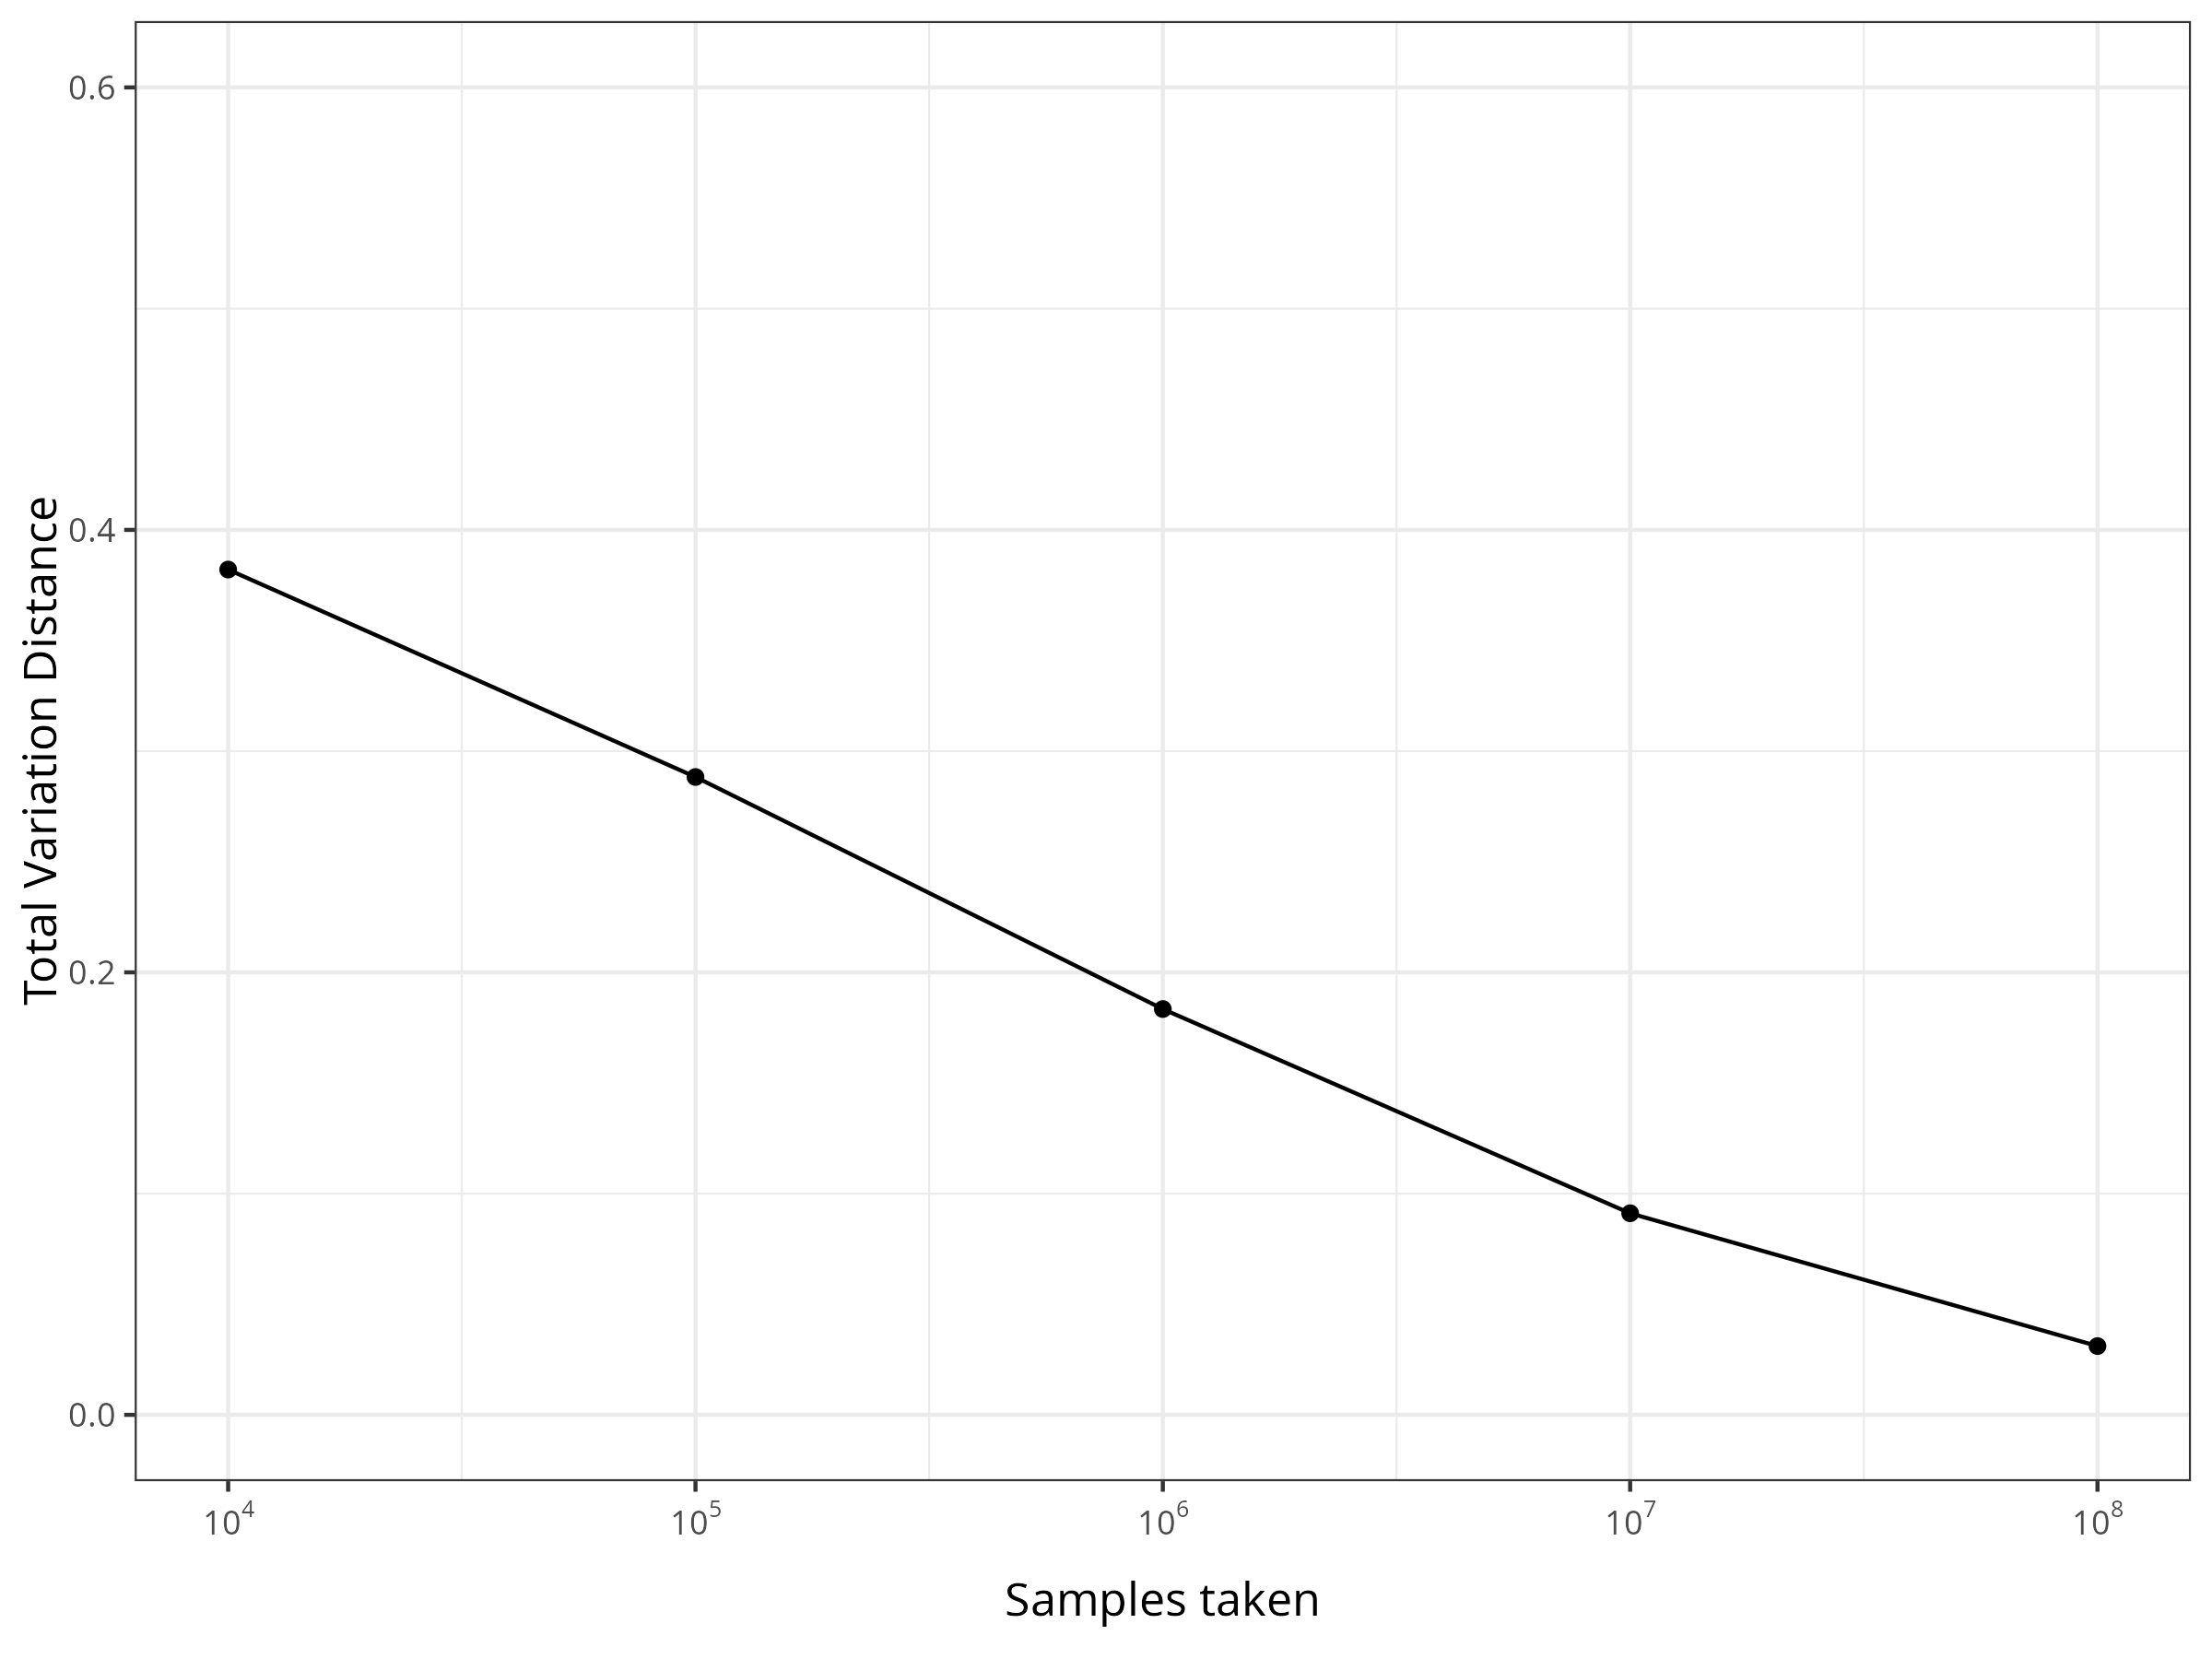
\includegraphics[width=\textwidth]{figures/tvd/rejection.png}
        \caption{Rejection Sampling}
    \end{subfigure}
    
    
    \caption{TVD test results for the different samplers.}
    \label{fig:tvd-graphs}
\end{figure}

\begin{table}[t]
    \centering
    \begin{tabularx}{\linewidth}{|>{\raggedright\arraybackslash}X|>{\raggedright\arraybackslash}X|>{\raggedright\arraybackslash}X|}
        \hline
        \textbf{Sampler} & \textbf{Total Variation Distance} & \textbf{Kolmogorov-Smirnov Statistic} \\
        \hline
        FIO (C) & 0.201 & 0.532 \\
        \hline
        Rejection-Inversion (Java) & 0.00963 & 0.0332 \\
        \hline
        YCSB (Java) & 0.0101 & 0.0338 \\
        \hline
        Sysbench (C) & 0.00963 & 0.0328 \\
        \hline
        Condensed Table Lookup (C++) & 0.0164 & 0.135 \\
        \hline
        Rejection (C++) & 0.031 & 0.0963 \\
        \hline
    \end{tabularx}
    \caption{Accuracy Results for $10^9$ samples}\label{tab:accuracy-results}
\end{table}

\paragraph{Analysis of Accuracy} 
All implementations but FIO and the condensed table lookup present very accurate tendencies when the sample size increases to the scales utilized in benchmarking, which confirm that they are safe to use. It now remains
to explain why both referenced algorithms are not quite as accurate. 

The FIO implementation likely presents systematic deviations from the expected values due to the hashing function used to preprocess the variates, as the variate generation itself follows exactly Jim Gray's pseudocode.
The choice of hashing function falls under the umbrella term "Jenkins Hash Function" (more specifically \textit{lookup3}, see \cite{jenkinsLookup3,HashFunctionHash}) to remap all generated variates before they are counted. Doing this, however,
introduces significant distortions in the distribution, since the aforementioned hash function is not perfect. Furthermore a good hash function should be mostly uniform, the
effect of which can be seen in the graph above as long intervals of constant probability occur. The drops are explained by the fact that eventually the lower-rank values eventually
"differ" enough their bit representation so as to be hashed to a different value. 

The case for the condensed table lookup is more complex. The algorithm is based on a table lookup with precision limited to $2^{30}$, or rather $5 \cdot 10^9$. This means that the algorithm is not able to generate
probabilities which only differ by a factor of $10^{-9}$ will be mapped to the same value. Testing for equality after this mapping yields that the probabilities are $99.9$ pairwise equal among all ranks, which is more
than sufficient to account for the long stretches of constant probability seen in Figure \ref{fig:pmf-graphs}. This effects gets amplified the lower the rank, which explains the ever stretching intervals of constant probability. A possible improvement would be 
to increase the precision of the table lookup, but this would also increase the memory requirements of the algorithm and make it closer to the naive approach.

\section{Evaluating Performance}
As already mentioned, evaluating performance is a tricky business. The main measure of interest is \textit{throughput}, which is the amount of variates generated 
in a time interval. What makes it complicated is controlling for external factors outside of the segment of code being tested. To this end, microbenchmarking is used and
common techniques are applied to avoid pitfalls \cite{AvoidingBenchmarkingPitfalls,beyerBenchmarkingResourceMeasurement2015}.

\subsection{Microbenchmarking}
Microbenchmarking is the process of measuring the performance of small code snippets, usually in the order of microseconds. The main goal is to measure the performance of 
the code in isolation, without the influence of other factors. Since the languages of interest are primarily C++, C and Java (see table \ref{tab:interpreter-versions}), 
the tools used to measure performance will be Google Benchmark \cite{GoogleBenchmarkMicrobenchmark} for C++ and C, and JMH \cite{AvoidingBenchmarkingPitfalls} for Java. 
For C++ and C applications, the following precations will be taken (for instruction on how to accomplish the following, see \cite{BenchmarkingTipsLLVM}):

\vspace{0.3cm}
\fbox{
    \centering
    \parbox{0.8\linewidth}{
        \begin{itemize}
            \item Set specific CPU core for the process
            \item Disable frequency scaling
            \item Disable turbo boost
            \item Limit the available memory to the process
            \item Warm-up runs 
        \end{itemize}
    }
    \label{microbenchmarking-precautions}
}
\vspace{0.3cm}

At last, it's important to define the runs. Since what is going to be measured is throughput, we define the duration of a single run to be 1 second. This will be repeated 30 times
and the average throughput will be calculated. Since the speed is invariant to domain size and distribution parameter, these are kept fixed at $10^8$ and 0.8, respectively.

For the Google Benchmark, the following command will be used to run the benchmarks (for more details on how to use the tool, see \cite{GoogleBenchmarkMicrobenchmark}):
\begin{lstlisting}
    ./benchmark --benchmark_repetitions=30 --benchmark_min_warmup_time=1.0
\end{lstlisting}

As a precaution for the sample generation not be optimized away, the function \verb|benchmark::DoNotOptimize| on the results of the computation was used. Similarly for the JMH (more details on \cite{AvoidingBenchmarkingPitfalls,jenkovJMHJavaMicrobenchmark}):
\begin{lstlisting}
    java -jar target/benchmarks.jar -bm thrpt -wi 10 -i 30 -f 1 -r 1
\end{lstlisting}

The results depende heavily on which JVM is used, but some common patterns exist to avoid making code be optimized away:              
\begin{itemize}
    \item Use the \verb|Blackhole| object to consume the results of the computation
    \item Use the \verb|@CompilerControl| annotation to avoid inlining
    \item Use the @\verb|State| annotation to avoid dead code elimination
\end{itemize}

\begin{table}[t]
    \centering
    \begin{tabular}{|c|c|c|c|}
        \hline
        \textbf{Sampler} & \textbf{Average Throughput (M/s)} & \textbf{Standard Deviation} \\
        \hline
        FIO (C) & 26.2 & 0.01 \\
        \hline
        Rejection-Inversion (Java) & 27.4 & 0.07 \\
        \hline
        YCSB (Java) & 29.9 & 0.14 \\
        \hline
        Sysbench (C) & 43.6 & 0.15 \\
        \hline
        Condensed Table Lookup (C++) & 45.2 & 0.06 \\
        \hline
        Rejection (C++) & 28.1 & 0.3 \\
        \hline
    \end{tabular}
    \caption{Microbenchmarking Results}\label{tab:microbenchmarking-results}
\end{table}

From the table \ref{tab:microbenchmarking-results}, we can recognize that the Condensed Table Lookup sampler is the fastest, which is to be expected given that the main operation is a table lookup,
while the cost gets offloaded to the initialization. The Sysbench sampler is the second fastest, which is expected given the overhead of the JVM.
But to further investigate why this difference is present, arun with a profiler is required. Running \verb|perf|\cite{PerfLinuxProfilinga} 
along with the JMH tool yields the following results for YCSB and Rejection-Inversion (Java). Only relevant lines are presented.

\begin{perfbox}{Rejection-Inversion (Java)}
\ttfamily
Baseline: 565.140.532.065 instructions 4,33  insn per cycle \\  
Sampler: 204.065.670.512  instructions  1,56 insn per cycle   \\
Sampler: 11.310.090  L1-dcache-load-misses  0,02\% of all L1-dcache accesses 
\end{perfbox}

\begin{perfbox}{YCSB}
\ttfamily
Baseline: 578.884.719.478 instructions 4,43 insn per cycle \\         
Sampler : 392.403.334.414  instructions 2,92  insn per cycle \\
Sampler: 339.375.866 L1-dcache-load-misses  0,43 \% of all L1-dcache accesses \\ 
Sampler: 789.273 L1-icache-load-misses 0,30\% of all L1-icache accesses 
\end{perfbox}

Given that both the baseline and the actual sample routine have similarly high IPC and low number of data and instruction cache misses, the lower throughput in Java is likely 
not caused by an inefficient implementatation, but rather by the overhead inherent to the JVM runtime, such as garbage collection, memory management and JIT compilation. These aspects
won't be explored further, which limits a rigorous conclusion. Nonetheless this points towards the JVM being responsible for the difference in performance.

\section{Overall Evaluation}

The results of the evaluation show that the Rejection-Inversion and Sysbench implementations are the most accurate and performant, closely followed by YCSB. 
The condensed lookup table is the fastest, but also less accurate. While currently the problems explored in the \textit{frequency ratio graphs} exclude it from further consideration, it could be improved by increasing the precision of the table lookup so as to make it competitive
with the other implementations. The FIO implementation is the least accurate and the slowest, which makes it unsuitable for further use. Lastly, the rejection algorithm is among the slowest and also not particularly accurate, which
excludes it from any further consideration. All in all, YCSB and Sysbench are the most viable choices for further use, as they are both accurate and performant and cover the use cases of database and file system benchmarks respectively.


`'